\documentclass[final]{cas-sc}
% Elsevier single-column CAS layout and journal-sized typography.
\usepackage[numbers]{natbib}
\renewcommand{\sfdefault}{lmss}
\renewcommand{\ttdefault}{lmtt}
\ExplSyntaxOn
\bool_gset_true:N \g_stm_nologo_bool
\ExplSyntaxOff
\renewcommand{\printorcid}{} % No ORCID identifiers have been supplied.
\ifdefined\pdfgentounicode
\input{glyphtounicode}
\pdfgentounicode=1
\fi
\usepackage{amsmath,amssymb,amsfonts,mathtools,amsthm,bm}
\usepackage{booktabs,graphicx,array,tabularx,longtable,float,url}
% Floats may follow their introduction, never precede it on the same page.
\usepackage{flafter}
\renewcommand{\topfraction}{0.9}
\renewcommand{\bottomfraction}{0.85}
\renewcommand{\textfraction}{0.1}
\hypersetup{hidelinks}
\hypersetup{pdfauthor={Ali Eslami and Jiangbo Yu}}
\usepackage[protrusion=true,expansion=false]{microtype}
\graphicspath{{figures/}{./}}
\allowdisplaybreaks
\setlength{\emergencystretch}{3em}
\interdisplaylinepenalty=2500
\theoremstyle{definition}
\newtheorem{assumption}{Assumption}
\theoremstyle{plain}
\newtheorem{theorem}{Theorem}
\newtheorem{proposition}{Proposition}
\newtheorem{lemma}{Lemma}
\newtheorem{corollary}{Corollary}
\newtheorem{remark}{Remark}
\theoremstyle{definition}
\newtheorem{definition}{Definition}
\newtheorem{problem}{Problem}
\theoremstyle{plain}
\floatstyle{ruled}
\newfloat{algorithm}{tbp}{loa}
\floatname{algorithm}{Algorithm}
\newcommand{\R}{\mathbb{R}}
% CAS uses plain appendix letters in cross-references.
\newcommand{\appref}[1]{Appendix~\ref{#1}}
\newcommand{\longpaperdetails}[1]{#1 of the \href{https://github.com/AlienEslami/agentic-perimeter-runtime-certification/blob/main/paper/main.pdf}{long version}}
\newcommand{\reproductiondetails}[1]{\href{https://github.com/AlienEslami/agentic-perimeter-runtime-certification/releases/tag/paper-2026-11-16-v2}{#1}~\cite{perimeterReproductionGuide}}
\shorttitle{Trustworthy agentic traffic control}
\shortauthors{A. Eslami and J. Yu}
% Compact running heads, with no invented publication metadata.
\makeatletter
\renewcommand{\ps@cas}{%
  \def\@oddhead{\footnotesize\itshape A. Eslami and J. Yu\hfill Trustworthy agentic traffic control}%
  \let\@evenhead\@oddhead
  \def\@oddfoot{\hfil\small\thepage\hfil}%
  \let\@evenfoot\@oddfoot}
\renewcommand{\ps@first}{%
  \let\@oddhead\@empty\let\@evenhead\@empty
  \def\@oddfoot{\hfil\small\thepage\hfil}%
  \let\@evenfoot\@oddfoot}
\makeatother
\pagestyle{cas}


% Reduced manuscript: verification structure and supporting appendices, 10 November 2026.
\begin{document}
\title[mode=title]{A Formal Guarantee for Trustworthy Agentic Traffic Control: A Multi-region Perimeter Case}
\author[mcgill]{Ali Eslami}
\ead{ali.eslami@mail.mcgill.ca}
\author[mcgill]{Jiangbo Yu}
\cormark[1]
\ead{jiangbo.yu@mcgill.ca}
\cortext[1]{Corresponding author.}
\affiliation[mcgill]{organization={Department of Civil Engineering, McGill University},
 addressline={817 Sherbrooke Street West}, city={Montreal}, state={Quebec},
 postcode={H3A 0G4}, country={Canada}}
\begin{abstract}
Urban perimeter control manages congestion by regulating traffic flows
between regions. Control plans may need to be revised as traffic conditions
and operating priorities change. Artificial intelligence (AI) agents can
support this process by interpreting operator instructions and using tools
to develop control plans. However, each new agent-proposed plan must remain
compatible with the evolving traffic state, uncertainty, and outstanding
service requirements. In this paper, we develop a dual-agent framework in
which an AI agent proposes plans and a rule-based supervisory agent checks
them before implementation. Under the stated traffic model, these checks
guarantee satisfaction of physical limits and service deadlines for accepted
plans despite bounded state-estimation and arrival-forecast errors. The
supervisory agent decides whether to accept a proposed plan, seek a modified
plan that meets the requirements, or reject the proposal while the current
plan continues under its existing guarantee.
Numerical studies demonstrate plan acceptance, repair, and replacement,
including under computation delays and agent-context errors. Overall, the
framework supports trustworthy AI for transportation by connecting adaptive
agent decisions to formally verified urban perimeter control.
\end{abstract}
\begin{keywords}
Urban perimeter control \sep Macroscopic fundamental diagram \sep
Constraint verification \sep Control under uncertainty \sep AI agents
\end{keywords}
\maketitle


\section{Introduction}
\label{sec:new-introduction}

Traffic control manages vehicle movements at intersections, along corridors,
and across urban networks to reduce delay and congestion
\cite{papageorgiou2003review}. At the regional scale, urban perimeter
control regulates traffic flows between areas of the network and their
surroundings. Restricting entry to a congested region can improve traffic
conditions inside it, but may also cause queues to grow at its boundary.
Control decisions must therefore account for both regional congestion and
boundary-queue storage \cite{haddad2017queues}. One approach to modeling regional traffic uses
the macroscopic fundamental diagram (MFD), which relates the number of
vehicles in a region to its aggregate outflow
\cite{geroliminis2008existence,daganzo2008analytical,geroliminis2011properties}.
Figure~\ref{fig:regional-traffic-overview} illustrates the regional traffic flows
and entry queues considered in this setting.

\begin{figure}[pos=!htb]
\centering
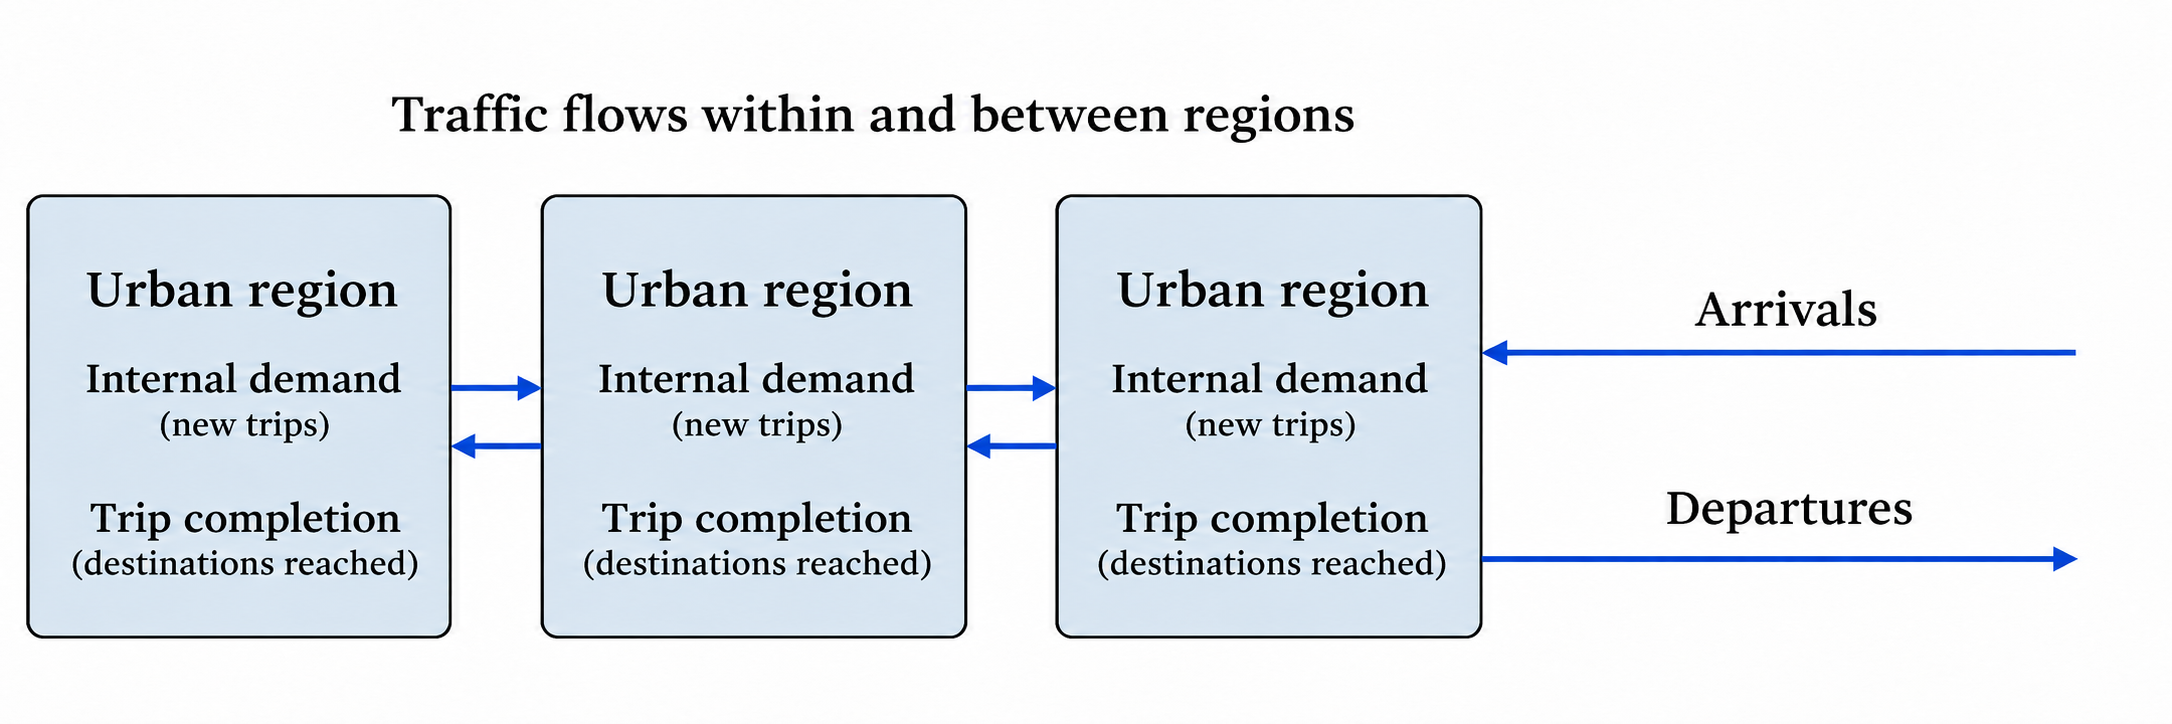
\includegraphics[width=\textwidth]{figures/regional_traffic_overview_matched_2026_11_16.png}
\caption{Urban perimeter control in a network of connected regions.
Arrivals and departures denote traffic entering and leaving the network.
Internal demand denotes trips starting within a region, while trip
completion denotes vehicles reaching their final destination there.
Arrows indicate the direction of traffic flow between regions and across
the network boundary, where perimeter control regulates these movements. Prepared with ChatGPT image generation
(OpenAI, accessed November 2026) and reviewed by the authors.}
\label{fig:regional-traffic-overview}
\end{figure}

Within this modeling framework, feedback control methods adjust boundary
flows in response to observed traffic conditions
\cite{keyvan2012gating,aboudolas2013perimeter}. Predictive methods use the
traffic model and demand forecasts to select control actions over a
prediction horizon \cite{geroliminis2013mpc,sirmatel2018economic}. Related
formulations explicitly account for boundary queues and their storage
limits \cite{haddad2017queues}. Robust control methods address uncertain
demand and limited traffic measurements, with stability and robustness
guarantees established under specified modeling assumptions
\cite{zhong2018robust,mohajerpoor2020hinf}. Earlier robust perimeter-control
formulations also address MFD uncertainty and uncertain destination
decomposition, including constrained interpolation-based control
\cite{haddad2014robust,haddad2015robust}.

Data-driven approaches have also been developed for perimeter control.
Reinforcement learning and adaptive dynamic programming use traffic
observations and the outcomes of control actions to learn control policies
\cite{chen2022dataefficient,chen2024iadp}. Multi-agent reinforcement
learning supports coordination across several regions and allows
different metering rates at individual boundary signals
\cite{zhou2023scalable,yu2025physicsperimeter}. Other formulations consider
controllers with different objectives. For example, Li et al.\ \cite{li2024beyond}
study non-cooperative interactions between controllers managing perimeter
flows and traffic generated within the network.

AI agents can also support traffic management by interpreting operator
instructions and using tools to develop control plans. TrafficGPT and
Open-TI demonstrate natural-language interaction with specialized
traffic-analysis tools \cite{trafficgpt2024,openti2024}. LA-Light couples
a large language model (LLM) with traffic-signal tools and checks the format of its proposed
decisions \cite{wang2024lalight}. Similar arrangements have been explored in robotics: SayCan connects language
instructions to robot skills \cite{saycan2023}, while VoxPoser uses
language-derived objectives and constraints to guide motion planning
\cite{voxposer2023}. For perimeter control, these precedents motivate
investigating agents that interpret instructions about regional priorities
and their duration, and use tools to develop and revise control plans.

An agent may use a planning tool with the wrong objective or base its
request on incorrect context. Even when the objective is appropriate, a
plan that satisfies the constraints in simulated cases may violate them
for other allowed initial states or arrival patterns. Traffic also
continues to evolve while a plan is being computed and checked, so a
replacement must be assessed for the conditions at the time of
implementation.

Existing assurance methods provide several relevant foundations
\cite{hobbs2023runtime}. Simplex architectures retain a verified backup
when a proposed control action cannot be accepted \cite{mehmood2022black}.
Control barrier functions enforce prescribed state constraints
\cite{ames2017}, while predictive safety filters assess future behavior
and modify proposals to preserve feasibility \cite{wabersich2021}.
Shielding uses a model and a formal specification to restrict a learner's
actions \cite{alshiekh2018}. Formal traffic-control methods exploit mixed
monotonicity to over-approximate reachable states and synthesize controllers
satisfying temporal-logic specifications \cite{coogan2017formal}.
Related reachability methods retain dependencies between uncertain states
\cite{coogan2020mixed,kochdumper2021sparse}. For LLM agents, specifications
on data flows and tool sequences provide a further level of runtime
enforcement \cite{doshi2026tools}.

Applying these ideas to agent-proposed perimeter control raises three
requirements. First, a check must cover every initial state and arrival
pattern allowed by the available information, not only simulated cases.
Second, each replacement must be checked against the conditions at its
implementation, after any computation delay, and against earlier service
requirements that remain in force. Third, the guarantee must hold even
when the agent's request uses the wrong objective or incorrect context.
The assurance methods above provide the foundations. To the best of
our knowledge, however, the
perimeter-control studies reviewed above do not provide a formulation
and guarantees for verifying agent-proposed plans under uncertainty
while maintaining physical constraints and service requirements as
plans change during operation.

We address these requirements for a network of urban regions with
exterior queues and density-dependent average speeds. A two-region model
provides the detailed formulation, with an extension to several entry
queues under fixed allocation assumptions. In the proposed dual-agent
architecture, an AI agent uses planning tools to propose control plans,
and a rule-based supervisory agent verifies them before implementation.
The supervisory agent bounds future regional accumulations and boundary
queues under state-estimation and arrival-forecast errors. It then
checks the physical constraints, such as storage limits, and the
service requirements, which are traffic targets with deadlines. A
proposal may be accepted, modified, or rejected. Until a verified
replacement starts, the current plan remains in use within the period
covered by its certificate.

The paper makes three main contributions:
\begin{enumerate}
\item We develop a method for verifying a perimeter-control plan for
every initial state and arrival error allowed by the stated bounds. The
method bounds future regional accumulations and the queue around a
predicted trajectory, and tightens these bounds using traffic
structure: independent queue bounds, the propagation of shared initial
uncertainty, and coordinates chosen for the admission regime.
Conservation coordinates cancel admission from balances that combine
regional accumulations with their queue shares, while destination
coordinates keep the regional balances independent of the queue under
capacity-limited admission with constant inputs within each control block.

\item We establish conditions under which the dual-agent architecture
maintains these guarantees as plans are replaced, delayed, or rejected.
The guarantees cover arbitrary agent requests under the stated traffic
and interface assumptions. If no verified replacement is ready in time,
the current plan continues under its existing guarantee.
\appref{sec:terminal-backup} gives additional conditions for continued
operation beyond a plan's specified duration.

\item We develop a procedure for modifying a rejected proposal using a
backup plan verified under the same conditions. Among the tested
alternatives that meet the requirements, the procedure selects the plan
whose control inputs differ least from the proposal.
\end{enumerate}

The paper is structured as follows:
Section~\ref{sec:new-problem} presents the traffic model and control
problem. Section~\ref{sec:new-agent} describes the two agents and their
planning and execution interface. Section~\ref{sec:new-certification} develops
constraint verification for one plan, and Section~\ref{sec:replacement-repair}
establishes guarantees for plan replacement, computation delays and repair,
each with proofs.
Section~\ref{sec:new-evidence} presents the numerical studies,
Section~\ref{sec:new-discussion} discusses operational implications, and
Section~\ref{sec:new-conclusion} concludes the paper.

\section{Traffic Model and Control Problem}
\label{sec:new-problem}

\subsection{Network traffic dynamics}
\label{app:new-model}

Consider a network of $N$ urban regions, indexed by $i=1,\ldots,N$, and
$n_q$ exterior entry queues, indexed by $q=1,\ldots,n_q$. Let $n_{ij}(t)$
be the number of vehicles in region $i$ at time $t$ whose final
destination is $j\in\{0,\ldots,N\}$, where $j=0$ denotes the exterior,
and let $z_q(t)$ be the number of vehicles waiting in queue $q$. Each
accumulation $n_{ij}$ corresponds to a region--destination pair $(i,j)$.
Vehicles with $j=i$ complete their trips in their current region,
vehicles with $j\ne i$ and $j\ge1$ travel to another region, and
vehicles with $j=0$ leave the network. The set
$\mathcal A\subseteq\{1,\ldots,N\}\times\{0,\ldots,N\}$ contains every
pair $(i,j)$ that can contain vehicles under the initial conditions,
internal demand, admissions and routing. For example, a two-region
network in which every destination is used has
$\mathcal A=\{(1,1),(1,2),(1,0),(2,2),(2,1),(2,0)\}$. The pairs in
$\mathcal A$ are written in a fixed order as
$(i_1,j_1),\ldots,(i_{n_{\rm acc}},j_{n_{\rm acc}})$, where
$n_{\rm acc}=|\mathcal A|$ is the number of pairs in $\mathcal A$ and
therefore the number of accumulations $n_{ij}$ in the model. The state
vectors are
\[
c(t)=\begin{bmatrix}
n_{i_1j_1}(t)\\ \vdots\\ n_{i_{n_{\rm acc}}j_{n_{\rm acc}}}(t)
\end{bmatrix}\in\R^{n_{\rm acc}},
\quad
z(t)=\begin{bmatrix}z_1(t)\\ \vdots\\z_{n_q}(t)\end{bmatrix}\in\R^{n_q},
\quad
x_{\rm net}(t)=\begin{bmatrix}c(t)\\z(t)\end{bmatrix}.
\]
The vector $c(t)$ contains the accumulations $n_{ij}(t)$ of all pairs
in $\mathcal A$, the vector $z(t)$ contains the queue lengths, and
$x_{\rm net}(t)\in\R^{n_{\rm acc}+n_q}$ is the network state. All counts are continuous aggregate quantities in
vehicles, time is in hours, and flow rates are in veh/h. A dot denotes
a time derivative and $\top$ transposition, vector inequalities and
absolute values are componentwise, and an identity matrix without a
stated dimension has the size required by its block.
\appref{app:notation} lists the notation.

The accumulations change through internal demand, local trip
completion, transfers between regions, exterior departures and
admission from the queues. The length of each queue increases at its
exterior arrival rate and decreases at its admission rate. The
resulting vehicle balances are
\begin{equation}
\dot x_{\rm net}
=\underbrace{\begin{bmatrix}
d^{\rm int}(t)+B(u)m(c)+P_a a(z,u)\\
\widehat\Lambda(t)-a(z,u)
\end{bmatrix}}_{f_{\rm net}(x_{\rm net},u,t)}
+\underbrace{\begin{bmatrix}0_{n_{\rm acc}\times n_q}\\I_{n_q}\end{bmatrix}}_{B_w}w(t).
\label{eq:network-state-space}
\end{equation}
In the regional balances (upper block), $d^{\rm int}(t)$ is the
internal demand. The term $B(u)m(c)$ accounts for local trip completion,
controlled transfers between regions, and exterior departures. Here
$m(c)$ contains the potential outflows and $u$ the control inputs.
The term $P_a a(z,u)$ is the admission from the queues, allocated to
the pairs in $\mathcal A$. In
the queue balances (lower block), $\widehat\Lambda(t)$ is
the forecast of the exterior arrivals, $w(t)$ is the error of this
forecast, and
$a(z,u)$ is the admission leaving the queues. The function
$f_{\rm net}$ therefore gives the dynamics under the forecast arrivals,
and the matrix $B_w\in\R^{(n_{\rm acc}+n_q)\times n_q}$ adds the
forecast error to the queue balances only, where
$0_{n_{\rm acc}\times n_q}$ is the zero matrix and $I_{n_q}$ is the
$n_q\times n_q$ identity matrix. The control vector and the terms of
\eqref{eq:network-state-space} are defined next.

The control inputs regulate transfers across region boundaries and
admission from exterior queues. Let $\mathcal E$ be the set of directed controlled boundaries
$(i,k)$, leading from region $i$ to a neighboring region $k\ne i$ or,
when $k=0$, to the exterior. Then
\[
u=\operatorname{col}\big((u_{ik})_{(i,k)\in\mathcal E},
                        (u_q^{\rm in})_{q=1}^{n_q}\big)
\in[0,1]^{|\mathcal E|+n_q},
\]
where $\operatorname{col}$ stacks its arguments in a fixed order,
$u_{ik}$ is the fraction of the flow assigned to boundary $(i,k)$ that
is allowed to cross it, and $u_q^{\rm in}$ is the fraction of the
entrance capacity of queue $q$ that is opened.

The internal demand vector follows the pair ordering of $c$:
\[
d^{\rm int}(t)=\operatorname{col}\big(d^{\rm int}_{i_1j_1}(t),\ldots,
d^{\rm int}_{i_{n_{\rm acc}}j_{n_{\rm acc}}}(t)\big)\in\R^{n_{\rm acc}},
\]
where $d_{ij}^{\rm int}(t)\ge0$ is the rate (veh/h) at which trips with
destination $j$ start inside region $i$.

The potential outflows follow from each region's speed--density
relationship. Region $i$ holds
$n_i=\sum_{j:(i,j)\in\mathcal A}n_{ij}$ vehicles on a total lane length
$\mathcal L_i>0$ (lane-km), so its density is
$\rho_i=n_i/\mathcal L_i$ (vehicles per lane-km). Let $V_i(\rho_i)$ be
the average speed at this density (km/h), with $V_i(\rho_i)\ge0$ and
$dV_i/d\rho_i\le0$, and let $\ell_i>0$ be the mean distance traveled
within the region (km). The potential outflow of the vehicles in region
$i$ with destination $j$, and its sum over destinations, are
\begin{equation}
\begin{aligned}
m_{ij}(c)&=\frac{n_{ij}V_i(n_i/\mathcal L_i)}{\ell_i},
\qquad (i,j)\in\mathcal A,\\
G_i(n_i)&=\sum_{j:(i,j)\in\mathcal A}m_{ij}(c)
=\frac{n_iV_i(n_i/\mathcal L_i)}{\ell_i},
\end{aligned}
\label{eq:class-potential-flow}
\end{equation}
both in veh/h. For $j=i$, $m_{ii}$ is the rate at which trips are
completed inside region $i$. For $j\ne i$, $m_{ij}$ is the rate at
which vehicles would leave region $i$ before routing and perimeter
control are applied. The function $G_i$ is the regional outflow
macroscopic fundamental diagram (MFD), relating total accumulation
$n_i$ to total potential outflow $G_i(n_i)$
\cite{geroliminis2008existence,mariotte2017comparisons}. For $n_i>0$
the first line reads $m_{ij}=(n_{ij}/n_i)\,G_i(n_i)$, so each
destination group contributes to the regional outflow in proportion to
its share of the accumulation
(Assumption~\ref{ass:regional-model}(b)). At $n_i=0$ it gives
$m_{ij}=0$ without division by $n_i$. Speed follows density
algebraically and is not an additional dynamic state, and $G_i$ may
have both increasing and decreasing branches. The critical
accumulation $n_i^{\rm crit}$ is the vehicle count at which $G_i$
reaches its capacity maximum, and $n_i^{\max}$ is an operational upper
limit on $n_i$. In the pair ordering of $c$, the potential outflows
form the vector
\[
m(c)=\operatorname{col}\big(m_{i_1j_1}(c),\ldots,
m_{i_{n_{\rm acc}}j_{n_{\rm acc}}}(c)\big)\in\R^{n_{\rm acc}}.
\]

Routing and perimeter control convert potential outflows into actual
flows. For each pair $(i,j)\in\mathcal A$ with $j\ne i$, the fixed
routing fraction $\mathsf R_{ik}^{(j)}$ is the share of $m_{ij}$
assigned to boundary $(i,k)$, with
\[
\mathsf R_{ik}^{(j)}\ge0,\qquad
\sum_{k:(i,k)\in\mathcal E}\mathsf R_{ik}^{(j)}=1.
\]
A forbidden route has zero fraction, an exterior exit ($k=0$) is used
only by vehicles leaving the network ($j=0$), and every interior route
with a nonzero fraction leads to a pair $(k,j)\in\mathcal A$. The flow
of destination-$j$ vehicles crossing boundary $(i,k)$ is
$\mathsf R_{ik}^{(j)}u_{ik}m_{ij}(c)$, so $u_{ik}=0$ blocks the assigned
flow and $u_{ik}=1$ permits its full value
(Assumption~\ref{ass:regional-model}(c)). Blocked vehicles remain in
region $i$, and crossing vehicles keep their destination $j$.

The matrix $B(u)\in\R^{n_{\rm acc}\times n_{\rm acc}}$ collects these
flows, so that $B(u)m(c)$ is the rate of change of $c$ caused by local
trip completion, interregional transfers and exterior departures. Let
$e_{ij}^{\rm acc}\in\R^{n_{\rm acc}}$ be the unit vector with a $1$ at
the position of pair $(i,j)$ in $c$ and zeros elsewhere, and set
$e_{0j}^{\rm acc}=0$ because vehicles that reach the exterior leave the
model. The column of $B(u)$ that multiplies $m_{ij}$ is
\[
B_{:,ij}(u)=
\begin{cases}
-e_{ii}^{\rm acc},&j=i,\\[3pt]
\displaystyle\sum_{k:(i,k)\in\mathcal E}
\mathsf R_{ik}^{(j)}u_{ik}\big(e_{kj}^{\rm acc}-e_{ij}^{\rm acc}\big),
&j\ne i.
\end{cases}
\]
The first case removes locally completed trips, which no input
controls. In the second case, each crossing flow is removed from group
$(i,j)$ and added to group $(k,j)$ of the receiving region, or leaves
the network when $k=0$.

Admission moves vehicles from the exterior queues into the regions.
Queue $q$ has a release time $\tau_q>0$ (h), a release coefficient
$\gamma_q^{\rm rel}=1/\tau_q$ (h$^{-1}$) and a full entrance capacity
$\kappa_q>0$ (veh/h). Its admission rate is
\[
a_q(z_q,u_q^{\rm in})
=\min\{\gamma_q^{\rm rel}z_q,\;\kappa_q u_q^{\rm in}\},
\]
the smaller of the rate at which its waiting vehicles can be released
and the opened part of its entrance capacity. The admission rates form
the vector
$a(z,u)=\operatorname{col}\big(a_1(z_1,u_1^{\rm in}),\ldots,
a_{n_q}(z_{n_q},u_{n_q}^{\rm in})\big)\in\R^{n_q}$. The fixed allocation
matrix $P_a\in\R_{\ge0}^{n_{\rm acc}\times n_q}$ distributes them over
the pairs in $\mathcal A$: its entry $(P_a)_{(i,j),q}$ is the fraction
of $a_q$ that enters region $i$ with destination $j$, and
\[
\mathbf 1_{n_{\rm acc}}^\top P_a=\mathbf 1_{n_q}^\top ,
\]
where $\mathbf 1_r$ is the vector of $r$ ones. Each admitted vehicle
therefore leaves one queue and joins one destination group, and
$P_a\,a(z,u)\in\R^{n_{\rm acc}}$ is the admission inflow to $c$.

Exterior arrivals enter the queue balances. Vehicles arrive at queue
$q$ at the rate $\Lambda_q(t)=\widehat\Lambda_q(t)+w_q(t)$, where
$\widehat\Lambda_q(t)$ is the forecast arrival rate and $w_q(t)$ is its
forecast error, referred to as the arrival error, all in veh/h. The
corresponding vectors are
\[
\begin{aligned}
\widehat\Lambda(t)&=\operatorname{col}\big(\widehat\Lambda_1(t),\ldots,
\widehat\Lambda_{n_q}(t)\big),\qquad
w(t)=\operatorname{col}\big(w_1(t),\ldots,w_{n_q}(t)\big),\\
\Lambda(t)&=\widehat\Lambda(t)+w(t),
\end{aligned}
\]
all in $\R^{n_q}$. The balance of queue $q$ in
\eqref{eq:network-state-space} is therefore
$\dot z_q=\widehat\Lambda_q+w_q-a_q$.

The model uses the following regional assumptions
\cite{geroliminis2011properties,geroliminis2013mpc,mohajerpoor2020hinf}:
\begin{assumption}
\label{ass:regional-model}
\begin{enumerate}
\renewcommand{\labelenumi}{(\alph{enumi})}
\item Each region admits a reproducible average speed--density
relationship over the operating range. Network geometry, the speed
functions, and routing shares are fixed model data.
\item Vehicles whose destination is their current region complete their
trips locally. Mean distances traveled within a region are taken to be
equal across destination groups and fixed, so each group's potential
outflow is proportional to its share of regional accumulation.
\item Each region has sufficient receiving capacity to accommodate
the modeled interregional transfers and admissions from exterior
queues under the operating conditions considered.
\item Exterior queues have finite storage limits $z_q^{\max}$,
measured in vehicles, and are represented as point queues.
\end{enumerate}
\end{assumption}

\begin{remark}
Consistent with the regional models in
\cite{zhong2018robust,mohajerpoor2020hinf}, receiving capacity is
assumed not to restrict the modeled inflows. Each regional MFD
depends on that region's own accumulation, while interregional
transfers depend on routing and perimeter control inputs.
Additional flow restrictions caused by congestion in the receiving
region, including spatial spillback, are outside the model.
\end{remark}

\subsection{Two-region model}
\label{sec:two-region-model}

The detailed construction uses the two-region network of
Figure~\ref{fig:two-region-network}. Region~1 exchanges traffic only with
Region~2, and Region~2 also borders the exterior. A single exterior
queue ($n_q=1$) feeds Region~2. Every destination is used in both
regions, so $\mathcal A$ contains all six region--destination pairs and
the accumulation vector of Section~\ref{app:new-model} becomes
\[
c(t)=\big(n_{11}(t),n_{12}(t),n_{10}(t),n_{22}(t),n_{21}(t),n_{20}(t)\big)^\top
\in\R^{6},
\]
with $n_{\rm acc}=6$. Because there is one queue, $z$, $a$, $\Lambda$,
$\widehat\Lambda$ and $w$ are scalars. The regional totals are
\begin{equation}
n_1=n_{11}+n_{12}+n_{10},\qquad n_2=n_{22}+n_{21}+n_{20}.
\label{eq:regional-class-totals}
\end{equation}

\begin{figure}[pos=!htb]
\centering
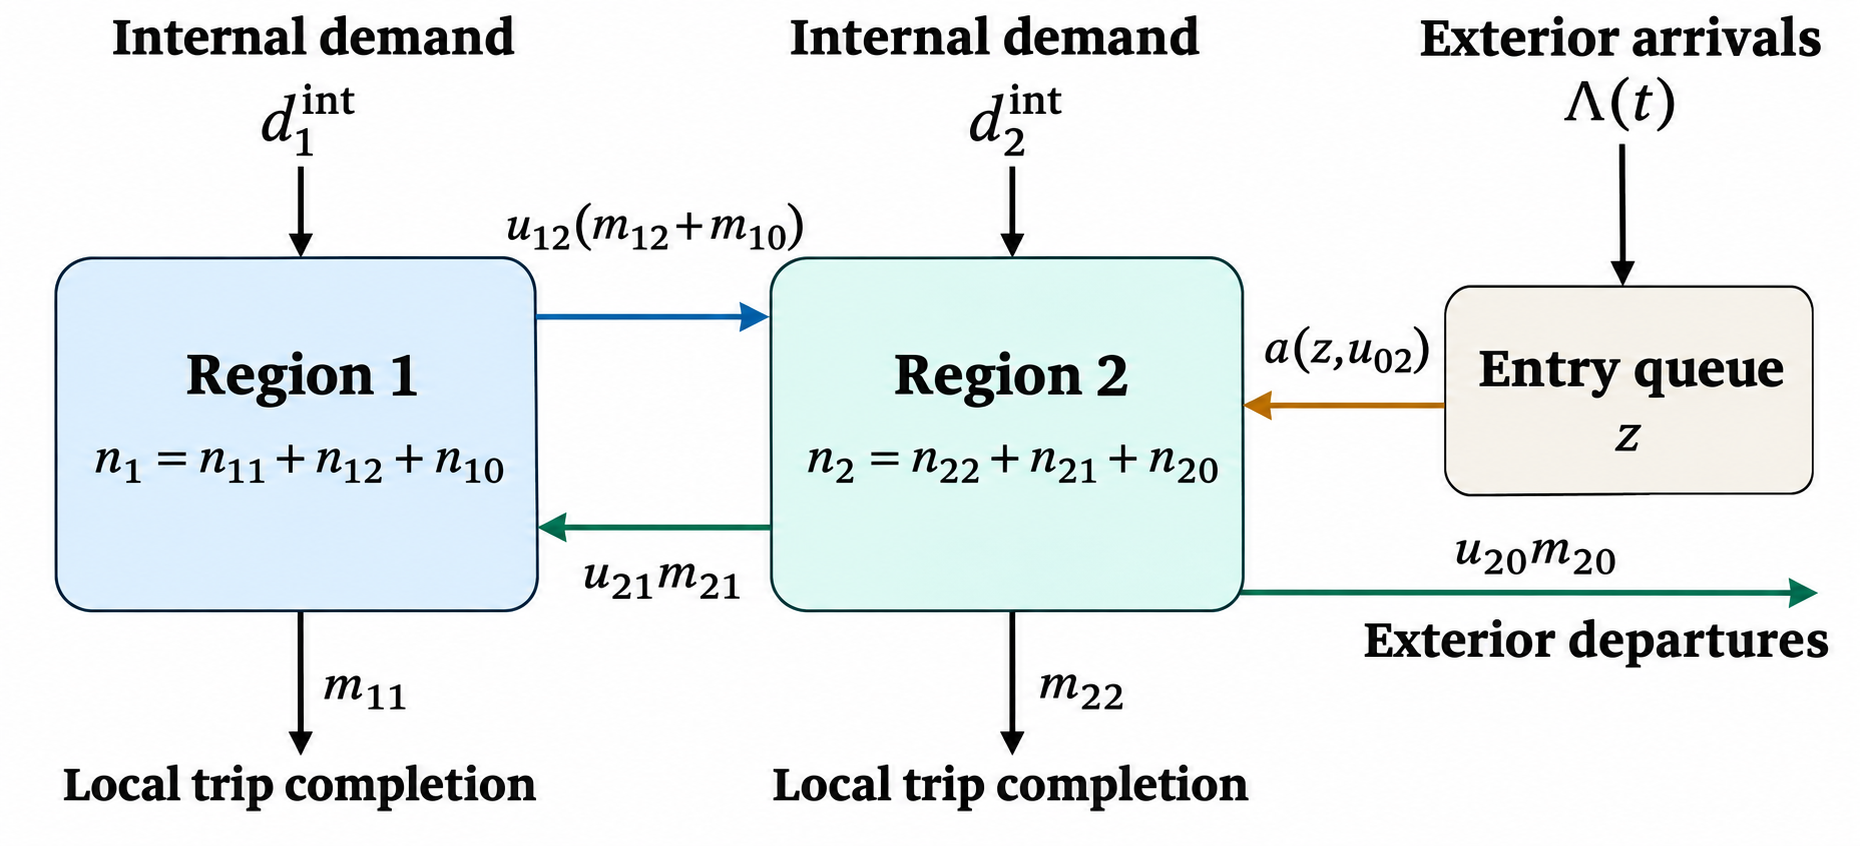
\includegraphics[width=0.76\textwidth]{figures/two_region_vehicle_flows_journal_2026_11_15.png}
\caption{Two-region traffic model. Regional accumulations $n_1,n_2$ and
the entry queue $z$ are measured in vehicles, and all arrow labels
denote rates in veh/h. Internal demand
$d_i^{\rm int}=\sum_j d_{ij}^{\rm int}$ generates trips within
Region~$i$, while exterior arrivals $\Lambda(t)$ join the queue.
Admission $a(z,u_{02})$ enters Region~2, with fractions $\pi$ and
$1-\pi$ joining $n_{21}$ and $n_{22}$, respectively. The potential
outflows $m_{ij}$ are restricted by perimeter control inputs $u_{ik}$
for transfers and exterior departures. Local trips finish at rates
$m_{11}$ and $m_{22}$. Vehicles retain their final destination when
transferring between regions. Destination index $0$ denotes the
exterior. Prepared with ChatGPT image generation
(OpenAI, accessed November 2026) and reviewed by the authors.}
\label{fig:two-region-network}
\end{figure}

Perimeter control acts on three boundaries,
$\mathcal E=\{(1,2),(2,1),(2,0)\}$, with inputs $u_{12}$, $u_{21}$ and
$u_{20}$. Each pair $(i,j)$ with $j\ne i$ has a single assigned route,
whose routing fraction equals one: vehicles counted in $n_{12}$ and
$n_{10}$ leave Region~1 through boundary $(1,2)$, vehicles in $n_{21}$
leave Region~2 through boundary $(2,1)$, and vehicles in $n_{20}$ leave
through the exterior exit $(2,0)$. The input $u_{12}$ therefore applies
to both $m_{12}$ and $m_{10}$. The entrance input of the queue,
$u_1^{\rm in}$ in Section~\ref{app:new-model}, is written $u_{02}$
because it controls entry from the exterior into Region~2.

The queue has release time $\tau_q>0$, where the subscript of
Section~\ref{app:new-model} is kept with $q=1$, and its entrance
capacity $\kappa_1$ is written $\kappa_{02}>0$. Its admission rate is
\begin{equation}
a(z,u_{02})=\min\{z/\tau_q,\;\kappa_{02}u_{02}\}.
\label{eq:new-admission}
\end{equation}
A fraction $\pi\in[0,1]$ of the admitted vehicles is destined for
Region~1 and joins $n_{21}$, and the remaining fraction $1-\pi$ is
destined for Region~2 and joins $n_{22}$. In the ordering of $c$, the
allocation matrix is therefore the column
\[
P_a=\big(0,0,0,1-\pi,\pi,0\big)^\top .
\]

With these data, the network dynamics \eqref{eq:network-state-space}
become
\begin{equation}
\begin{aligned}
\dot n_{11}&=d_{11}^{\rm int}-m_{11}+u_{21}m_{21},\\
\dot n_{12}&=d_{12}^{\rm int}-u_{12}m_{12},\\
\dot n_{10}&=d_{10}^{\rm int}-u_{12}m_{10},\\
\dot n_{22}&=d_{22}^{\rm int}-m_{22}+u_{12}m_{12}+(1-\pi)a,\\
\dot n_{21}&=d_{21}^{\rm int}-u_{21}m_{21}+\pi a,\\
\dot n_{20}&=d_{20}^{\rm int}-u_{20}m_{20}+u_{12}m_{10},\\
\dot z&=\widehat\Lambda+w-a,
\end{aligned}
\label{eq:destination-class-balances}
\end{equation}
where $m_{ij}=n_{ij}V_i(n_i/\mathcal L_i)/\ell_i$ is the potential
outflow in \eqref{eq:class-potential-flow} and $a=a(z,u_{02})$. The
six regional balances follow Mohajerpoor et
al.~\cite{mohajerpoor2020hinf}, building on
\cite{geroliminis2013mpc,zhong2018robust}. The exterior queue replaces
direct gated exterior demand with admission from stored waiting
vehicles.

The potential outflows can be specified through either the speed
function $V_i$ or the outflow MFD $G_i$, which are equivalent
descriptions once $\mathcal L_i$ and $\ell_i$ are given. In the
numerical studies, the empirical outflow MFD is the supplied model
data, and \eqref{eq:class-potential-flow} gives the corresponding
speed function
\begin{equation}
V_i(\rho)=\ell_i\frac{G_i(\mathcal L_i\rho)}{\mathcal L_i\rho}
\quad(\rho>0),\qquad
V_i(0)=\ell_i G_i'(0).
\label{eq:speed-from-mfd}
\end{equation}
The value at zero follows by continuous extension, using $G_i(0)=0$.
The balances depend on the speed only through the regional
per-vehicle outflow rate $v_i(n_i)=V_i(n_i/\mathcal L_i)/\ell_i$. When
both regions share the outflow curve $G_1=G_2=G$, they share this rate:
\begin{equation}
v(n)=\frac{G(n)}{n}=\frac{V_i(n/\mathcal L_i)}{\ell_i}\quad(n>0),
\qquad v(0)=G'(0),\qquad m_{ij}=n_{ij}v(n_i).
\label{eq:per-vehicle-outflow-rate}
\end{equation}
The quantity $v$ is a per-vehicle outflow rate in h$^{-1}$, whereas
$V_i$ is an average speed in km/h. For distinct regional curves, the
verification uses each region's $v_i$ and bounds on its derivatives
over the state ranges being checked.

The analysis uses coordinates in which the regional operating limits
appear directly. We replace $n_{12}$ and $n_{21}$ by the totals $n_1$
and $n_2$, and order the state and the inputs as
\begin{equation}
\begin{aligned}
x&=(n_1,n_2,n_{11},n_{22},n_{10},n_{20},z)^\top ,\\
u&=(u_{12},u_{21},u_{02},u_{20})^\top .
\end{aligned}
\label{eq:new-state}
\end{equation}
This input ordering places the entrance input before the exterior-exit
input. Since $n_{12}=n_1-n_{11}-n_{10}$ and
$n_{21}=n_2-n_{22}-n_{20}$, the vectors $x$ and
$x_{\rm net}=(c^\top,z)^\top$ describe the same seven independent
vehicle counts. Summing the three balances of each region in
\eqref{eq:destination-class-balances} gives the regional-total balances
\begin{equation}
\begin{aligned}
\dot n_1&=d_1^{\rm int}-m_{11}-u_{12}(m_{12}+m_{10})+u_{21}m_{21},\\
\dot n_2&=d_2^{\rm int}-m_{22}+u_{12}(m_{12}+m_{10})-u_{21}m_{21}
+a-u_{20}m_{20},
\end{aligned}
\label{eq:regional-flow-balances}
\end{equation}
where $d_i^{\rm int}=d_{i1}^{\rm int}+d_{i2}^{\rm int}+d_{i0}^{\rm int}$
is the total internal demand of Region~$i$. Together with the balances
of $n_{11}$, $n_{22}$, $n_{10}$, $n_{20}$ and $z$ in
\eqref{eq:destination-class-balances}, these give
\begin{equation}
\dot x=f(x,u,t)+e_7w(t),\qquad e_7=(0,0,0,0,0,0,1)^\top .
\label{eq:new-plant}
\end{equation}
The function $f$ contains the right-hand sides of these seven balances
at zero arrival error, in the ordering of
\eqref{eq:new-state}, and $e_7$ adds the arrival error to the
queue balance. Throughout the two-region analysis, $e_j$ denotes the
unit vector selecting state component $j$.

\subsection{Control plans and operating constraints}
\label{sec:physical-constraints}

A control plan $P$ covers an execution interval $[t_0,E]$, from its
start time $t_0$ to its end time $E$. At every time in this interval it
specifies the control input $u(t)$, either directly or through a
state-feedback law. The input must remain in the admissible set
\begin{equation}
\mathcal U=\big\{u:\;0\le u\le1,\quad
|u_{21}-u_{12}|\le\delta_1^u,\quad
|u_{20}-u_{02}|\le\delta_2^u\big\}
\label{eq:new-gates}
\end{equation}
for all $t\in[t_0,E]$, where $u=(u_{12},u_{21},u_{02},u_{20})^\top$ as
in \eqref{eq:new-state}. The first condition bounds every input
between $0$ and $1$. The limits $\delta_1^u,\delta_2^u\in[0,1]$ bound
the difference between the two inputs of opposite directions at the
same boundary: $u_{12}$ and $u_{21}$ between the regions, and $u_{02}$
and $u_{20}$ between Region~2 and the exterior. These difference bounds
follow Mohajerpoor et al.~\cite{mohajerpoor2020hinf} and reflect that
opposite-direction movements can share signal phases.

The state is constrained by nonnegativity of every vehicle count and by
the storage available in the regions and in the queue:
\[
\begin{aligned}
&n_{11},\,n_{10},\,n_{22},\,n_{20}\ge0,\qquad
n_1-n_{11}-n_{10}\ge0,\qquad n_2-n_{22}-n_{20}\ge0,\\
&0\le n_i\le n_i^{\max}\quad(i=1,2),\qquad 0\le z\le z^{\max}.
\end{aligned}
\]
The two differences in the first line are the accumulations $n_{12}$
and $n_{21}$, which are not components of $x$ in
\eqref{eq:new-state}. The bound $n_i^{\max}$ is the operational
accumulation limit of Section~\ref{app:new-model}, and $z^{\max}$
denotes the storage limit $z_1^{\max}$ of the single exterior queue
(Assumption~\ref{ass:regional-model}(d)), both in vehicles.

We refer to these state constraints and the input constraints in
\eqref{eq:new-gates} collectively as the physical constraints. Each of
them is a linear inequality in $(x,u)$, and written as one-sided
inequalities they number $24$: twelve on the inputs and twelve on the
state.

\subsection{Control objectives and service requirements}
\label{sec:benchmark-formulation}

For a plan $P$, an initial state $x_0=x(t_0)$ and an arrival-error
signal $w$, let $x_P(t;x_0,w)$ and $u_P(t;x_0,w)$ denote the state and
the applied control input at time $t\in[t_0,E]$. Here $w$ denotes the
whole signal on $[t_0,E]$, while $w(t)$ is its value at time $t$. The
components $n_{1,P}$, $n_{2,P}$ and $z_P$ of $x_P$ are the two regional
totals and the queue length along this trajectory. The arguments
$(x_0,w)$ are omitted when the planning scenario specifies them.

The network-efficiency objective, identified by the subscript Q,
minimizes the total time spent in both regions and in the exterior
queue:
\begin{equation}
J_Q(P;x_0,w)=\int_{t_0}^{E}M_P(t;x_0,w)\,dt,\qquad
M_P=n_{1,P}+n_{2,P}+z_P.
\label{eq:benchmark-queue-cost}
\end{equation}
The integrand $M_P$ is the total accumulation $M=n_1+n_2+z$ along the
trajectory of plan $P$, in vehicles, so the cost is in vehicle-hours.

The regional-priority objective, identified by the subscript D, gives
Region~2 a temporary priority by weighting its accumulation with a
factor $p\ge1$:
\begin{equation}
J_D(P;x_0,w)=\int_{t_0}^{E}
\big(n_{1,P}(t)+p\,n_{2,P}(t)+z_P(t)\big)\,dt.
\label{eq:benchmark-priority-cost}
\end{equation}
The three trajectory components are evaluated at the same $(x_0,w)$,
the cost is again in vehicle-hours, and $p=1$ recovers $J_Q$.

These objectives express preferences. In contrast, \emph{service
requirements} are traffic targets that must be met at specified
deadlines. There are $n_s$ service requirements, and requirement
$r=1,\ldots,n_s$ has the form
\begin{equation}
g_r^\top x(T_r)\le\eta_r,\qquad T_r\in[t_0,E],
\label{eq:new-service}
\end{equation}
where the dimensionless coefficient vector
$g_r=(g_{r,1},\ldots,g_{r,7})^\top$ follows the ordering of $x$ and
selects the traffic quantity, $\eta_r$ is its limit in vehicles, and
$T_r$ is the deadline. For example, a Region~1 vehicle-count target
$\eta$ at plan end is specified by $g_r=e_1$, $T_r=E$ and
$\eta_r=\eta$, giving $n_1(E)\le\eta$. Service requirements remain
binding when regional priorities change, and a target or deadline can
be modified only by an operator instruction.

\subsection{Uncertainty and verification requirements}
\label{sec:problem-uncertainty}

A plan must be verified for every initial state and every arrival
error that the available information allows. For a plan starting at
$t_0$, the initial state is known only to lie in a set
$\mathcal I_{t_0}$ that contains the actual traffic state $x(t_0)$.
When an estimate $\widehat x_{t_0}$ with a componentwise error bound
$d_x$ is available, this set is the box
\begin{equation}
\mathcal I_{t_0}=\{x:\;|x-\widehat x_{t_0}|\le d_x\},
\label{eq:benchmark-contract}
\end{equation}
where $d_x=(d_{x,1},\ldots,d_{x,7})^\top\in\R^7_{\ge0}$ is measured in
vehicles and follows the ordering of $x$ in
\eqref{eq:new-state}. Its component $d_{x,k}$ is the largest
allowed absolute difference between state component $k$ and its
estimate, that is, the half-width of the box in that component. The
estimate and its error bound are supplied externally.

The arrival error is bounded in absolute value by $\bar w\ge0$ (veh/h)
throughout the execution interval. The allowed error signals therefore
form the set
\[
\mathcal W=\{w:[t_0,E]\to\R:\; w\text{ is measurable},\quad
|w(t)|\le\bar w\ \ \forall t\in[t_0,E]\}.
\]
The forecast $\widehat\Lambda$ and the bound $\bar w$ are chosen so
that all allowed arrivals $\widehat\Lambda(t)+w(t)$ remain nonnegative.

The requirements that a plan must meet are collected in two sets. The
$n_c$ physical constraints of Section~\ref{sec:physical-constraints} form
\[
\mathcal P_{\rm phys}=\{H_jx+J_ju\le\beta_j^{\rm phys}:\;j=1,\ldots,n_c\},
\]
where $H_j\in\R^{1\times7}$ and $J_j\in\R^{1\times4}$ are the state
and input coefficient rows and $\beta_j^{\rm phys}\in\R$ is the limit
of constraint $j$. The $n_s$ service requirements in
\eqref{eq:new-service} form
\[
\mathcal O=\{(T_r,g_r,\eta_r):\;r=1,\ldots,n_s\}.
\]

\begin{definition}
\label{def:planning-contract}
A \emph{planning specification} is the tuple
\[
\mathcal C=(\mathcal I_{t_0},\bar w,f,\mathcal P_{\rm phys},\mathcal O,[t_0,E]),
\]
which consists of the initial-state set, the arrival-error bound, the
dynamics $f$ in \eqref{eq:new-plant}, including the
arrival forecast, the physical constraints, the service requirements
and the execution interval.
\end{definition}

\begin{definition}
\label{def:robust-feasibility}
A \emph{robustly feasible} plan has a well-defined trajectory
throughout $[t_0,E]$ for every allowed initial state and arrival error,
and satisfies all physical constraints throughout this interval and all
service requirements at their deadlines. The set of these plans is
\begin{equation}
\begin{aligned}
\mathcal F_{\mathcal C}=\{P:\ &\forall x_0\in\mathcal I_{t_0},\ w\in\mathcal W,\\
&H_jx_P(s;x_0,w)+J_ju_P(s;x_0,w)\le\beta_j^{\rm phys}\\
&\quad\text{for all }s\in[t_0,E]\text{ and physical constraints }j,\\
&g_r^\top x_P(T_r;x_0,w)\le\eta_r\quad
\text{for all service requirements }r\}.
\end{aligned}
\label{eq:benchmark-feasible-set}
\end{equation}
\end{definition}

Constraint verification requires a computable check that establishes
these conditions for every allowed initial state and arrival error.

\begin{definition}
\label{def:feasibility-certificate}
Given a plan $P$ and a planning specification $\mathcal C$, a completed
constraint-verification check returns
$\mathsf{Cert}_{t_0}(P\mid\mathcal C)\in\{0,1\}$. A value of $1$ means
that the plan has been verified, while $0$ means that the check has not
established constraint satisfaction. A plan is called \emph{certified}
when $\mathsf{Cert}_{t_0}(P\mid\mathcal C)=1$. The procedure must accept only
robustly feasible plans:
\[
\mathsf{Cert}_{t_0}(P\mid\mathcal C)=1\quad\Longrightarrow\quad
P\in\mathcal F_{\mathcal C}.
\]
Its accepted set therefore satisfies
\begin{equation}
\widehat{\mathcal F}_{\mathcal C}
=\{P:\ \mathsf{Cert}_{t_0}(P\mid\mathcal C)=1\}\subseteq\mathcal F_{\mathcal C}.
\label{eq:benchmark-certifiable-set}
\end{equation}
\end{definition}

Planning tools seek low cost under forecast or scenario conditions,
while verification establishes constraint satisfaction for all allowed
initial states and arrival errors. An inconclusive check leaves robust
feasibility undecided. A constraint violation for some allowed initial
state and arrival error establishes that the plan is not robustly
feasible.

\paragraph{Problem definition}
\label{prob:supervised-planning}
Given the traffic model, a planning
specification, and a sequence of proposed plans, design a supervisory
procedure that performs the following three functions.
\begin{enumerate}
\item \textbf{Constraint verification.} Construct a computable
procedure that accepts a plan only when it meets the specification for
every allowed initial state and arrival error.
\item \textbf{Plan modification.} When a proposal is not certified,
seek a modified plan that passes the same check, using a backup
certified for the applicable specification. We refer to this
modification procedure as \emph{repair}.
\item \textbf{Successive replacement.} Across successive requests and
computation delays, activate a proposed or repaired plan only when a
matching certificate is completed by the plan start time and covers
every possible state at plan start and every pending service
requirement. Otherwise, continue the current plan within its original
execution interval.
\end{enumerate}

\section{Dual-Agent Architecture for Perimeter Control}
\label{sec:new-agent}

\subsection{Architecture overview}
\label{sec:architecture-overview}

The architecture in Figure~\ref{fig:new-architecture} separates plan
proposal from plan execution. The operator issues instructions and
priorities. The AI agent interprets these instructions and requests
plans from numerical planning and repair tools. A deterministic
\emph{tool interface} validates each request and forwards the
resulting candidate plans to both agents. The rule-based supervisory
agent, called the \emph{supervisor}, checks these candidates and
decides which plan is executed. The \emph{execution interface} applies
the supervisor's decision to the traffic system, and observations of
the traffic system update the traffic information.

\begin{figure}[pos=!htb]
\centering
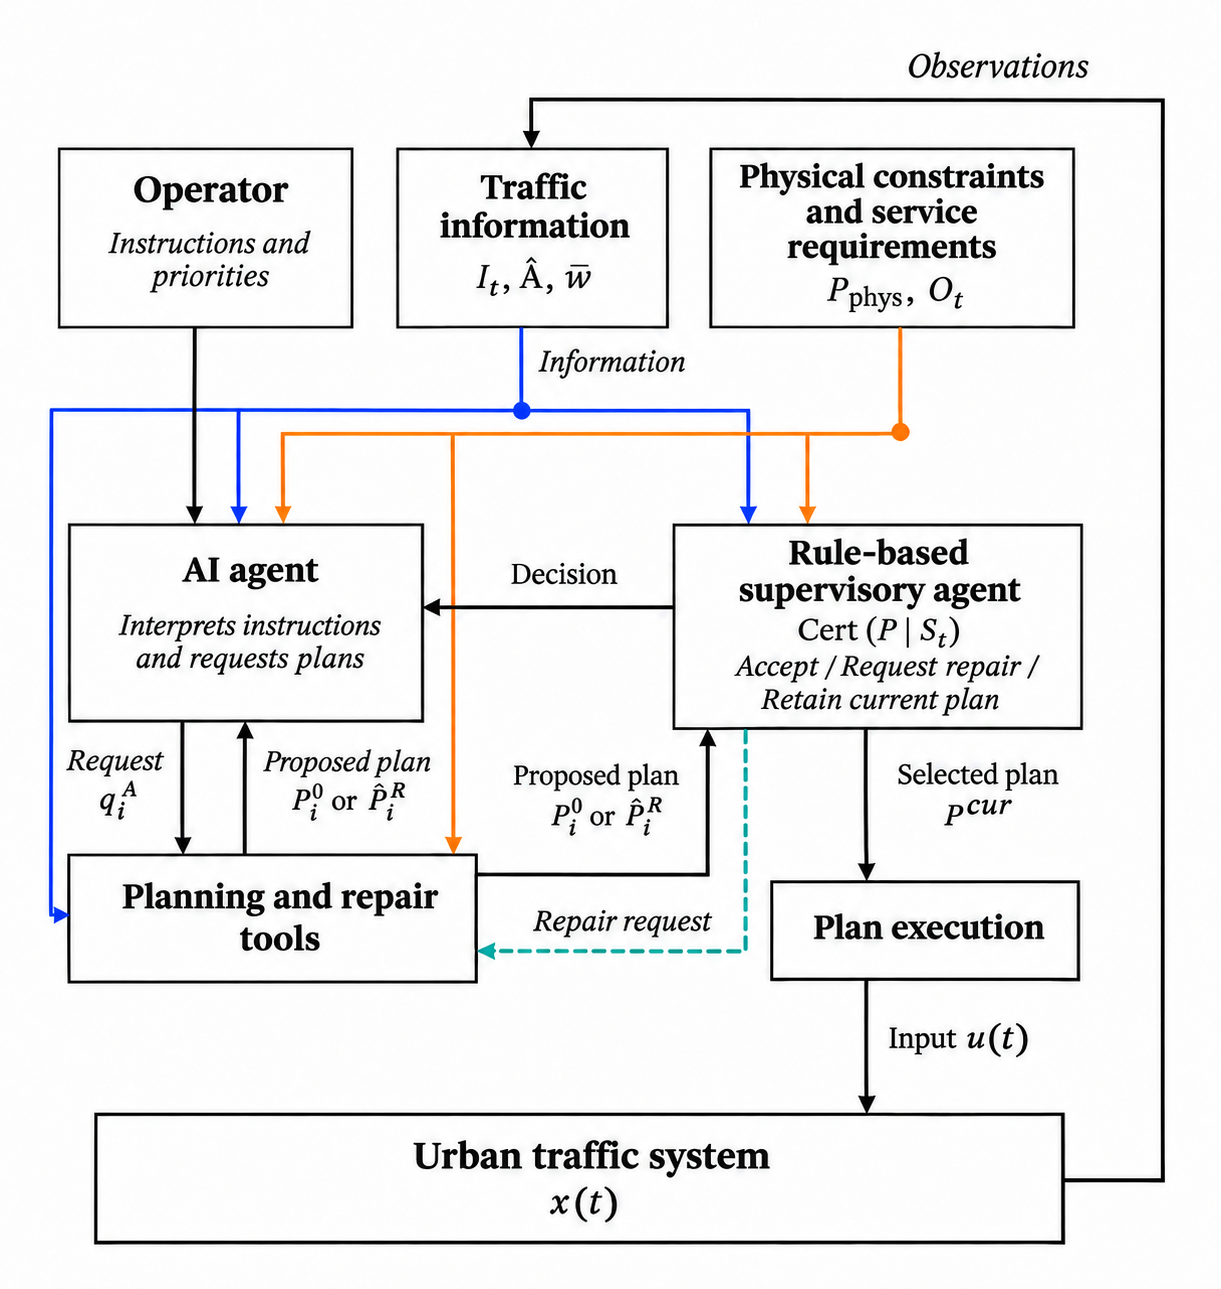
\includegraphics[width=0.90\textwidth]{figures/dual_agent_architecture_simplified_2026_11_16.png}
\caption{Proposed dual-agent architecture. Blue paths carry the
supplied state set $\mathcal I_t$, arrival forecast $\widehat\Lambda$
and error bound $\bar w$; orange paths carry physical constraints
$\mathcal P_{\rm phys}$ and pending service requirements $\mathcal O_t$.
These inputs reach the AI agent, planning tools and rule-based
supervisory agent directly. At decision $i$, with plan start time
$t_i$, the AI agent forms planning request $q_i^{A}$. The tools return
proposed plans $P_i^{0}$ or repair candidates $\widehat P_i^{R}$ to
both agents. The supervisory agent uses the constraint check
$\mathsf{Cert}$ and decision record $\mathcal S_{t_i}$ to select the
current plan $P^{\rm cur}$ for execution with control input $u(t)$.
The dashed line denotes automatic repair requests. The observation
loop represents measurement feedback. Prepared with ChatGPT image generation
(OpenAI, accessed November 2026) and reviewed by the authors.}
\label{fig:new-architecture}
\end{figure}

The traffic information, the physical constraints and the service
requirements are supplied independently of the AI agent. They reach
both agents and the numerical tools directly, and the supervisor
checks every candidate against them.

The agents interact through a sequence of decisions, indexed by $i$.
In decision $i$, the agent issues a request at time $t_i^{\rm req}$,
the tools return a proposed plan $P_i^{0}$, and the supervisor checks
it for a possible plan start time $t_i\ge t_i^{\rm req}$, also called
the activation time. The proposal is activated only if it meets the
supervisor's acceptance conditions in Section~\ref{sec:supervisory-agent}.
Otherwise, the current plan continues under its existing certificate
until its specified end time. Traffic evolves continuously during
computation, service deadlines keep their absolute times, and only
finitely many decisions occur on a finite interval. A subscript $i$ on
a plan, set or record refers to decision $i$, for example
$\mathcal I_i=\mathcal I_{t_i}$, whereas indices on traffic variables
retain their regional or boundary meaning.

This separation of responsibilities determines how proposals reach
execution, and it implements the three functions of the problem
definition in Section~\ref{sec:problem-uncertainty}. The supervisor performs
constraint verification and governs successive replacement, and the
repair tool proposes modified plans, which the supervisor verifies in
the same way. The resulting guarantee concerns physical constraints
and service requirements; correct interpretation of the requested
objective is evaluated separately. Whereas hierarchical perimeter
control coordinates decisions across control levels
\cite{ramezani2015heterogeneity,su2023hierarchical}, the proposed interface
requires each plan to pass verification before implementation. It can
receive proposals from a learned controller, optimizer or human, with
the LLM demonstration in \appref{sec:task-state-live} providing one
such proposer.

\subsection{Representation of control plans}
\label{sec:control-plans}

The plans exchanged in this architecture are blockwise. A plan divides
its execution interval into $N_b$ time blocks and specifies a
perimeter control law for each block:
\begin{equation}
\begin{aligned}
P&=\big((\tau_b,\tau_{b+1},k_b,K_b)\big)_{b=0}^{N_b-1},
\qquad t_0=\tau_0<\cdots<\tau_{N_b}=E,\\
u_P(t)&=k_b+K_bx(t),\qquad t\in[\tau_b,\tau_{b+1}).
\end{aligned}
\label{eq:control-plan-tuple}
\end{equation}
Here $b$ indexes the control blocks, $\tau_b$ are their boundary
times, $k_b$ is the constant input offset of block $b$, and $K_b$ is
its state-feedback gain. In the two-region model, $k_b\in\R^{4}$ and
$K_b\in\R^{4\times7}$. We also write $u_P(t,x)$ when the state
argument of the plan's control law is shown explicitly.

The formulation includes open-loop schedules and affine
state-feedback laws. With $K_b=0$, the plan is a sequence of
perimeter control inputs, each held constant over its block, which
gives an open-loop control schedule. Target feedback
$u=u_b^\star+K_b(x-x_b^\star)$, where $x_b^\star$ and $u_b^\star$ are
the chosen reference state and input, corresponds to
$k_b=u_b^\star-K_bx_b^\star$.

Execution follows three conventions. States remain continuous at
input changes, and constraints are checked on both sides. The last
block supplies the left-limit input at its end time $E$ unless a
certified successor starts there. For $K_b\ne0$, execution assumes
access to the true state: activation uncertainty is covered by the
initial set, and feedback from estimates would require additional
input-error bounds.

The certificate of a plan covers its execution interval $[t_0,E]$.
Operation beyond $E$ requires a certified replacement or a verified
terminal policy, that is, a feedback policy certified for operation
after the plan ends, as specified in \appref{sec:terminal-backup}.

\subsection{AI agent and planning tools}
\label{sec:agent-requests}

At request time $t_i^{\rm req}$, the agent interprets the operator's
instruction using the supplied traffic information and service
requirements, together with its interaction history. This history
contains earlier instructions, tool responses and supervisory
feedback, and the agent's memory is a stored summary of it.

The agent requests a plan by specifying the regional priority, its
remaining duration, and the weights on regional and queue
accumulations. The tool interface converts this request into the
numerical planning request $q_i^{A}$, where the superscript $A$
identifies an agent request, and returns $q_i^{A}=\bot$ for an invalid
request. Two input formats are used. In the history-only format, the
agent supplies these quantities directly and the tool interface
validates them. In the task-record format, the agent is additionally
given a task record $\theta_i$, which stores the active priority, its
absolute end time $T^{\rm prio}$ and the interrupted priorities, so
that priorities are tracked across interruptions. The request
compiler $\mathsf{Comp}$ then applies the operation rules in
Table~\ref{tab:task-operations}, updates $\theta_i$ and forms $q_i^{A}$.
Interrupted priorities retain their absolute end times, so their
remaining durations continue to decrease. These priority changes
leave pending service requirements unchanged.

Given $q_i^{A}$, the planning tool returns a proposed plan $P_i^{0}$
for the requested objective of Section~\ref{sec:benchmark-formulation}. It uses
a model predictive control (MPC) formulation
\cite{geroliminis2013mpc} to solve a finite-horizon problem when
requested. Once accepted and activated, the schedule continues until
its specified end time unless a newly verified replacement is activated. A second tool, the repair tool, seeks a modified
plan when a proposal fails verification; it uses the supervisor's
record and is described in Section~\ref{sec:supervisory-agent}.
\appref{sec:task-state-live} compares the two input formats and
tests corrupted memory, in which the stored summary is replaced by
misleading instructions about priorities, limits or execution.

\subsection{Supervisory agent}
\label{sec:supervisory-agent}

The supervisor keeps the information needed to check and execute
plans in the decision record
\[
\mathcal S_t=(\mathcal I_t,\mathcal W_t,\mathcal O_t,P_t^{\rm cur},
\mathcal H_t,P_t^{B},t,\mathsf{ver}_t).
\]
Here $\mathcal I_t$ is the supplied or propagated state set at time
$t$, $\mathcal W_t$ is the arrival-error family, and $\mathcal O_t$
contains the accepted service requirements whose deadlines have not
passed. The current plan $P_t^{\rm cur}$ retains its original
certificate $\mathcal H_t$, its end time $E_{\rm cur}$ and its reachable sets,
including all component certificates when the initial set is
subdivided. The certificate records the verified state bounds and the
conditions under which they apply. The repair backup is $P_t^{B}$, or
$\bot$ when unavailable, $t$ is the time of the record, and the
identifier $\mathsf{ver}_t$ records the model, forecast,
physical-constraint and service-requirement versions, including
deadline changes.

These fields and a candidate end time $E$ define a planning
specification $\mathcal C(\mathcal S_t,E)$ in the sense of
Definition~\ref{def:planning-contract}. The check of a plan $P$
that starts at $t$ is therefore written
\[
\mathsf{Cert}_t(P\mid\mathcal S_t)
=\mathsf{Cert}_t\big(P\mid\mathcal C(\mathcal S_t,E)\big).
\]

Before a candidate $P$, either a proposal or a repair, replaces the
current plan at $t_i$, the supervisor requires three conditions.
\begin{enumerate}
\renewcommand{\labelenumi}{(\roman{enumi})}
\item The check has passed and was completed by the plan start time:
\[
\mathsf{Cert}_{t_i}(P\mid\mathcal S_{t_i})=1,\qquad
t_{\rm ready}\le t_i,
\]
where $t_{\rm ready}$ is the certificate completion time, with
$t_{\rm ready}=\infty$ when no completed result is available.
\item The certificate matches the plan to be implemented: the checked
coefficients, plan start time, model and data versions, and
authorized requirements agree with execution.
\item The certificate covers the possible states at plan start and
the arrival errors, and includes all pending service requirements.
\end{enumerate}
The state set $\mathcal I_{t_i}$ used in the check must therefore be
available early enough for the check to be completed by $t_i$. The
supervisor can obtain this set by propagating the current plan's
certified state bounds to the activation time. A fresh estimate for
the activation time does not remove the timely-completion requirement. If a condition fails, the current plan
continues under its existing certificate until its end time
$E_{\rm cur}$. A new service requirement is accepted only when the
selected plan covers it.

\begin{remark}
\label{rem:recertification}
Failure to recertify the current plan from an enlarged state set does
not invalidate its original certificate. While its original
assumptions hold, the plan may continue to its original end time
unless a verified replacement starts earlier.
\end{remark}

When a proposal is rejected, repair can be invoked automatically by
the supervisor or requested by the agent following feedback. In both
modes the repair tool returns
\begin{equation}
\widehat P_i^{R}=\mathsf{RepairTool}\big(P_i^{0},P_i^{B},
\mathcal S_{t_i},\mathcal G_{\rm rep}\big),
\label{eq:repair-tool-interface}
\end{equation}
where $P_i^{0}$ is the proposal, $P_i^{B}$ is the backup,
$\mathcal G_{\rm rep}$ is a finite grid of interpolation weights
between them, and $\widehat P_i^{R}$ is the returned repair candidate.
Repair requires a backup that passes under the same conditions as the
candidates. The remaining current plan can serve this role if it
passes the new check; otherwise a newly certified plan is needed. Both
modes use the same verification and implementation rules:
conditions (i)--(iii) apply to original and repaired proposals alike.
Section~\ref{sec:predictive-repair} defines the search, which operates on
piecewise-constant control schedules ($K_b=0$).
Section~\ref{sec:new-incident-protocol} uses the automatic mode, and
\appref{sec:task-state-live} uses agent-requested repair.

\subsection{Execution rules and assumptions}
\label{sec:execution-interface}

In addition to the traffic-model assumptions in
Assumption~\ref{ass:regional-model}, verification relies on the
following conditions on the externally supplied data and on the
interfaces.

\begin{assumption}
\label{ass:trusted-inputs}
The externally supplied data satisfy the following conditions:
\begin{enumerate}
\renewcommand{\labelenumi}{(\alph{enumi})}
\item Each externally supplied state set contains the actual state at
its timestamp.
\item The stated arrival-error bounds hold.
\item Traffic follows \eqref{eq:new-plant} under the
model and uncertainty assumptions of the active certificate.
\item Physical constraints and service requirements are authorized by
the operator.
\item These data reach the tools and the supervisor independently of
agent requests and memory.
\end{enumerate}
\end{assumption}

\begin{assumption}
\label{ass:supervisory-separation}
The execution interface satisfies the following conditions:
\begin{enumerate}
\renewcommand{\labelenumi}{(\alph{enumi})}
\item Agent outputs cannot modify independently supplied data, pending
requirements, or the decision record.
\item Only the supervisor authorizes activation, and execution uses
the checked coefficients, timing, and model version.
\item A new service requirement becomes pending only when the selected
plan covers it.
\item Invalid requests, failed checks, and late results leave the
current plan and its original certificate in use, while their
assumptions hold, until the plan ends or a later certified replacement
starts.
\end{enumerate}
\end{assumption}

Algorithm~\ref{alg:agent-execution} summarizes one decision under
these assumptions. Section~\ref{sec:new-certification} develops the check
$\mathsf{Cert}$ used in its Step~\ref{step:checking}.
Section~\ref{sec:replacement-repair} shows that, for every sequence of
agent requests, execution under the algorithm
satisfies the physical constraints and service requirements over the
intervals covered by the selected certificates
(Corollary~\ref{cor:agent-independent-execution}). Operation beyond those intervals
requires the replacement or terminal policy of
Section~\ref{sec:control-plans}.

\begin{algorithm}[!htbp]
\caption{Planning requests and certified execution}
\label{alg:agent-execution}
\begin{minipage}{\linewidth}
\small
\textbf{Input:} current certified plan and record $\mathcal S_t$,
operator requests, independently supplied traffic data and
requirements, agent history, and $\theta_i$ when used.\\
\textbf{Output:} selected plan and certificate, updated record and
feedback.\\
For each request at $t_i^{\rm req}$, while the current plan remains in
force:
\begin{enumerate}
\setlength{\itemsep}{2pt}
\item\label{step:request} \textbf{Tool interface and agent:} process priority end times
and form $q_i^{A}$, using $\mathsf{Comp}$ for the task-record variant
or direct validation otherwise. If $q_i^{A}=\bot$, retain the current
decision record and return feedback.
\item\label{step:planning} \textbf{Planning tool:} use $q_i^{A}$ and the independent data
to generate $P_i^{0}$. The tool interface forwards it to the
supervisor and returns plan information to the agent.
\item\label{step:activation} \textbf{Supervisor:} choose $t_i$ and assemble
$\mathcal S_{t_i}$ from a propagated containing state set or a valid
estimate for the activation time (Proposition~\ref{prop:planned-handover}),
available early enough for the check to be completed by $t_i$.
Preserve accepted deadlines, including those during computation.
\item\label{step:checking} \textbf{Supervisor and repair tool:} apply
$\mathsf{Cert}_{t_i}(P_i^{0}\mid\mathcal S_{t_i})$ using
Theorem~\ref{thm:new-plan-enclosure} and, when used,
Proposition~\ref{prop:structure-plan}. The sequential procedure tests a fixed
sequence of bounding configurations using the complete-cover rule
\eqref{eq:portfolio-cover-rule}. After rejection, invoke repair only if
requested by the agent or enabled automatically. Check every repair
and its backup under the same conditions.
\item\label{step:installation} \textbf{Supervisor:} activate a
candidate $P$ only when $\mathsf{Cert}_{t_i}(P\mid\mathcal S_{t_i})=1$,
the matching certificate is complete by $t_i$
($t_{\rm ready}\le t_i$), execution data match, and all pending
requirements are covered. Otherwise retain the current plan,
certificate and end time. Accept a new service requirement only when
the selected plan covers it.
\item\label{step:feedback} \textbf{Interfaces:} return feedback, update history and the
decision record, and execute within the interval covered by the
selected plan's certificate.
\end{enumerate}
\end{minipage}
\end{algorithm}

\section{Verification of Perimeter-Control Plans}
\label{sec:new-certification}

The supervisor verifies a proposed plan by constructing sets that
contain every traffic state allowed by the specified uncertainty. These
sets are called \emph{state enclosures}. The construction follows a
predicted trajectory, proposes a tube around it, shows that no allowed
trajectory can leave this tube, and then checks the constraints on the
whole tube. If one of these steps cannot be established, the check
returns $0$, which leaves robust feasibility undecided
(Definition~\ref{def:feasibility-certificate}).

Sections~\ref{sec:verification-block-data} and~\ref{sec:coordinate-choices} state the
block dynamics and the coordinates used. Section~\ref{app:new-enclosure-proof}
gives the basic check of one plan (Theorem~\ref{thm:new-plan-enclosure}), and
Section~\ref{sec:structure-certificate} tightens it for constant inputs
(Proposition~\ref{prop:structure-plan}). Sections~\ref{sec:combining-checks}
and~\ref{sec:network-extension} combine several checks and treat several
entry queues. Section~\ref{sec:replacement-repair} then carries the
guarantee through plan replacement, computation delays and repair,
providing the checks used in Algorithm~\ref{alg:agent-execution}.
The detailed construction uses the two-region state $x$. Its
mathematical foundations are validated numerics
\cite{tucker2011validated}, generalized Jacobians
\cite{clarke1990optimization}, and comparison arguments
\cite{khalil2002nonlinear,farina2000positive}. \appref{sec:terminal-backup}
gives terminal-continuation conditions, and \appref{sec:repair-cost-bound}
gives a conditional repair-cost bound.

\subsection{Block dynamics and constraints}
\label{sec:verification-block-data}

For each block $b$ of a plan defined in
Section~\ref{sec:control-plans}, substituting the block law into the
two-region dynamics \eqref{eq:new-plant} gives
\begin{equation}
u_b(x)=k_b+K_bx,\qquad
\dot x=f_b(x,t)+e_7w(t),\qquad |w(t)|\le\bar w,
\label{eq:new-plan-data}
\end{equation}
where $f_b(x,t)=f(x,u_b(x),t)$ is the nominal block field, obtained
with the arrival forecast $\widehat\Lambda$, and
$\Lambda(t)=\widehat\Lambda(t)+w(t)$. The forecast is continuous and
piecewise affine, and $w$ is any measurable signal satisfying the
bound. Feedback uses the exact state, as specified in
Section~\ref{sec:control-plans}.

The fitted outflow and the piecewise-affine admission law are locally
Lipschitz in the state and measurable in time, so each bounded
measurable arrival error gives a unique local, absolutely continuous
trajectory. The internal demand rates $d_{ij}^{\rm int}(t)$ are assumed
measurable and locally bounded, so their integrals over finite
intervals are finite. The polynomial model is evaluated over the candidate
bounding sets, including any parts outside the physical domain;
acceptance still requires the physical constraints to hold. The
verification below uses derivative bounds on either outflow branch and
does not require the speed-monotonicity assumption.

For the physical constraints $\mathcal P_{\rm phys}$ of
Section~\ref{sec:problem-uncertainty}, substitution of the block law gives
\begin{equation}
h_{jb}^\top x\le\beta_{jb},\qquad
h_{jb}^\top=H_j+J_jK_b,\qquad
\beta_{jb}=\beta_j^{\rm phys}-J_jk_b,
\label{eq:new-physical-rows}
\end{equation}
where $j=1,\ldots,n_c$ indexes the physical constraints. The service
requirements do not involve the input and remain
$g_r^\top x(T_r)\le\eta_r$ for $r=1,\ldots,n_s$, as in
\eqref{eq:new-service}.

\subsection{Queue admission and coordinate choice}
\label{sec:coordinate-choices}

Admission transfers vehicles from an exterior queue into a receiving
region. Combining each receiving accumulation with its allocated queue
share cancels that transfer from their joint balance. We first state
the result for the general network of Section~\ref{app:new-model} and
then specialize it to two regions. Write
$F(c,u,t)=d^{\rm int}(t)+B(u)m(c)$ for the regional balance term
without admission, so that \eqref{eq:network-state-space} reads
$\dot c=F(c,u,t)+P_aa$ and $\dot z=\Lambda-a$, with fixed $P_a$ and
$\mathbf 1^\top P_a=\mathbf 1^\top$.

The following proposition establishes this cancellation and shows that
the combined accumulations count every internal and waiting vehicle
once. The subscript $c$ in $y_c$ identifies the regional block of the
transformed state; its queue block remains $z$.

\begin{proposition}
\label{prop:network-localization}
For fixed $P_a$, the invertible coordinate map
\begin{equation}
L_a=\begin{bmatrix}I&P_a\\0&I\end{bmatrix},\qquad
y=L_a\begin{bmatrix}c\\z\end{bmatrix}
=\begin{bmatrix}c+P_az\\z\end{bmatrix}
\label{eq:network-transform}
\end{equation}
gives
\begin{equation}
\dot y_c=F(y_c-P_az,u,t)+P_a\Lambda,\qquad \dot z=\Lambda-a.
\label{eq:network-transformed-flow}
\end{equation}
Thus explicit admission terms occupy only the $n_q$ queue coordinates.
No invertible linear transformation can confine these $n_q$ independent
channels to fewer than $n_q$ scalar coordinates. Moreover,
$\mathbf 1_{n_{\rm acc}}^\top y_c=\mathbf 1_{n_{\rm acc}}^\top c
+\mathbf 1_{n_q}^\top z$, so the combined accumulations count all
internal and waiting vehicles exactly once.
\end{proposition}

\begin{proof}
The inverse is $c=y_c-P_az$. Differentiation and the admission
incidence give
\[
\dot y_c=F(c,u,t)+P_aa+P_a(\Lambda-a)=F(c,u,t)+P_a\Lambda,\qquad
L_a\begin{bmatrix}P_a\\-I\end{bmatrix}
=\begin{bmatrix}0\\-I\end{bmatrix}.
\]
The original incidence has rank $n_q$ because of its lower block $-I$.
An invertible map preserves rank, while having fewer than $n_q$ nonzero
rows would lower it. Finally, $\mathbf 1^\top P_a=\mathbf 1^\top$ gives
the stated total-accumulation identity.
\end{proof}

Recovering the six destination accumulations from the two-region state
$x$ and applying Proposition~\ref{prop:network-localization} gives
\begin{equation}
\begin{aligned}
y=Lx=(&n_{11},n_{12},n_{10},n_{22}+(1-\pi)z,\\
&n_{21}+\pi z,n_{20},z)^\top .
\end{aligned}
\label{eq:new-conservation-coordinates}
\end{equation}
For this conservation-coordinate choice, $L$ first recovers $(c,z)$
from $x$ and then applies $L_a$. The regional accumulations are
recovered by the inverse map
\begin{equation}
\begin{aligned}
n_1&=y_1+y_2+y_3, & n_2&=y_4+y_5+y_6-y_7,\\
n_{11}&=y_1, & n_{22}&=y_4-(1-\pi)y_7,\\
n_{10}&=y_3, & n_{20}&=y_6,\qquad z=y_7.
\end{aligned}
\label{eq:new-inverse-coordinates}
\end{equation}
Let $b_a=(0,1,0,1-\pi,0,0,-1)^\top$ be the admission incidence, which
collects the coefficients of $a$ in the balances of $x$. Then
\begin{equation}
Lb_a=-e_7,\qquad Le_7=(0,0,0,1-\pi,\pi,0,1)^\top .
\label{eq:new-conservation-incidence}
\end{equation}
Thus $n_1+n_2+z=\sum_{i=1}^{6}y_i$, and admission cancels from the
combined accumulations. For example,
\[
\frac{d}{dt}(n_{21}+\pi z)=d_{21}^{\rm int}-u_{21}m_{21}+\pi\Lambda .
\]
This cancellation avoids bounding the same uncertain admission twice
with opposite signs. Regional outflow still depends on the transformed
state, and the queue remains necessary to recover regional
accumulations.

The useful coordinate choice depends on what limits admission. On the
queue-limited branch, admission is set by the waiting vehicles through
$a=z/\tau_q$, so uncertainty in $z$ also affects regional inflow.
Conservation coordinates remove this shared admission term, although
arrival error still enters through $Le_7w$. On the capacity-limited
branch with constant inputs, $a=\kappa_{02}u_{02}$ is independent of
$z$, and arrival error does not enter the regional equations.
Destination coordinates
\[
\widetilde Lx=(n_{11},n_{12},n_{10},n_{22},n_{21},n_{20},z)^\top
\]
preserve this separation. The two representations therefore exploit
different features of the admission dynamics, and neither dominates in
general.

The containment proofs below apply to any fixed invertible $L$
retaining $z$ as its last coordinate, with the Jacobian, disturbance,
predictor and constraint bounds recomputed accordingly. Keeping the
queue coordinate permits intersection with the independent scalar queue
bounds of Section~\ref{sec:structure-certificate}.

\subsection{Trajectory bounds and constraint verification}
\label{app:new-enclosure-proof}

We bound the deviation from a reference trajectory on each verification
interval. The plan is partitioned at control changes, forecast-slope
changes, service deadlines and intermediate verification times.
Interval $l$ starts at $t_l$ and has duration $h_l=t_{l+1}-t_l$, and
local time $s$ corresponds to $t_l+s$.

On interval $l$, the differentiable predictor $\mathbf p_l$ provides
the reference, and two vectors bound the deviation from it:
\[
\begin{aligned}
\mathbf p_l(t)&=\big(p_{1l}(t),\ldots,p_{7l}(t)\big)^\top ,\\
r_l&=\big(r_{1l},\ldots,r_{7l}\big)^\top ,\qquad
R_l=\big(R_{1l},\ldots,R_{7l}\big)^\top .
\end{aligned}
\]
The predictor follows the physical-state ordering in
\eqref{eq:new-state}, while the radii bound
transformed-coordinate errors. The vector $r_l\ge0$ bounds the error at
the beginning of the interval,
$|L(x(t_l)-\mathbf p_l(t_l))|\le r_l$, with absolute values taken
componentwise. The propagated state set at $t_l$ is
$\mathbf p_l(t_l)+L^{-1}[-r_l,r_l]$, represented by a box in the
transformed error coordinates; we call it the \emph{propagated box}.
Initially, $\mathbf p_0(t_0)=\widehat x_{t_0}$ and $r_0\ge|L|d_x$, so
this set covers the initial-state box
\eqref{eq:benchmark-contract}; a predictor that starts elsewhere also
requires $r_0$ to cover the offset of its center. After the first
interval, $r_l$ is propagated from the preceding one. The positive vector $R_l$ specifies candidate error
bounds for the whole interval, called \emph{trial radii}. The
corresponding \emph{trial set}
$\mathbf p_l(t)+L^{-1}[-R_l,R_l]$ is intended to contain every possible
state throughout the interval. The implementation uses a quadratic
predictor from the nominal dynamics, Jacobian and forecast slope, and
generates the trial radii iteratively
(\appref{app:verified-arithmetic}); they support acceptance only after
the tests below pass.

To verify the proposed bound, we account for the predictor's derivative
mismatch and bound the transformed Jacobian over the entire trial set
and interval:
\begin{equation}
\begin{aligned}
a_{il}^{\rm cmp}&\ge\sup\,(LD_xf_bL^{-1})_{ii},\\
b_{ijl}^{\rm cmp}&\ge\sup\,|(LD_xf_bL^{-1})_{ij}|\quad(j\ne i),\\
\delta_{il}&\ge\sup_t\,|(Lf_b(\mathbf p_l(t),t)-L\dot{\mathbf p}_l(t))_i|.
\end{aligned}
\label{eq:new-local-bounds}
\end{equation}
Here $D_xf_b$ is the Jacobian with respect to the state, and the
indices $i,j$ on these derivative bounds identify state components.
The superscript cmp abbreviates comparison, and $\delta_{il}$ bounds
component $i$ of the predictor's derivative mismatch on interval $l$.
The diagonal comparison coefficients can account for error decay as
well as growth, while the off-diagonal coefficients bound coupling
between components. At an admission-branch boundary, the generalized
Jacobian lies in the convex hull of the smooth branch limits, so both
branches are included unless verified bounds exclude one over the
whole trial set. Any exclusion of an admission branch must hold along
every segment joining predictor and possible state, because these
segments determine the derivative bounds used in the proof.

Together with predictor and arrival errors, these coefficients give the
comparison functions
\begin{equation}
\begin{aligned}
c_{il}^{\rm cmp}(R_l)&=\sum_{j\ne i}b_{ijl}^{\rm cmp}R_{jl}
+\delta_{il}+|(Le_7)_i|\bar w,\\
\phi_{il}(s)&=e^{a_{il}^{\rm cmp}s}r_{il}
+\chi(a_{il}^{\rm cmp},s)\,c_{il}^{\rm cmp}(R_l),\\
\chi(\mu,s)&=\begin{cases}
(e^{\mu s}-1)/\mu,&\mu\ne0,\\
s,&\mu=0.
\end{cases}
\end{aligned}
\label{eq:new-component-comparison}
\end{equation}
Here $c_{il}^{\rm cmp}$ bounds the combined contribution of coupling
between state components, predictor mismatch and arrival error, while
$\phi_{il}$ is the scalar comparison radius. The function
$\chi(\mu,s)$ is the integral of $e^{\mu\tau}$ over $0\le\tau\le s$.

Two tests use these functions. The first keeps the error within the
trial set, and the second checks each physical constraint over that
set:
\begin{align}
\max\{r_{il},\phi_{il}(h_l)\}&<R_{il}\quad\text{for every }i,
\label{eq:new-self-inclusion}\\
\sup_{t\in[t_l,t_l+h_l]}h_{jb}^\top\mathbf p_l(t)
+|h_{jb}^\top L^{-1}|R_l&\le\beta_{jb}.
\label{eq:new-affine-support}
\end{align}
To continue with a new predictor at the next interval, account for the
change of center using the recentering bound $\delta_l^{\rm rec}$
(superscript rec),
\begin{equation}
\delta_l^{\rm rec}\ge|L(\mathbf p_l(t_{l+1})-\mathbf p_{l+1}(t_{l+1}))|,
\label{eq:new-recentering-bound}
\end{equation}
and propagate $r_{i,l+1}=\phi_{il}(h_l)+\delta_{il}^{\rm rec}$. At
control changes, the constraints for the next control block are also
checked on the box propagated to that boundary. At a service deadline,
the predictor center $\mathbf p(T_r)$ and the error bound propagated to
that time, $r(T_r)$, give
\begin{equation}
g_r^\top\mathbf p(T_r)+|g_r^\top L^{-1}|\,r(T_r)\le\eta_r .
\label{eq:new-service-support}
\end{equation}
In this test the subscript $r$ is the requirement index, while
$r(T_r)$ is the radius vector at the deadline.

In summary, the interval check of a plan performs the following steps
and returns $1$ only if every test passes.
\begin{enumerate}
\item Partition the execution interval and form the initial predictor
and radius $r_0$.
\item On each interval $l$, choose $\mathbf p_l$ and $R_l$, establish
the bounds \eqref{eq:new-local-bounds} over the trial set, and evaluate
\eqref{eq:new-component-comparison}.
\item Test containment \eqref{eq:new-self-inclusion} and the physical
constraints \eqref{eq:new-affine-support}.
\item Propagate the radius using \eqref{eq:new-recentering-bound}. At a control
change, also check the next block's constraints on the propagated box;
at a service deadline, test \eqref{eq:new-service-support}.
\end{enumerate}
The following theorem shows that the interval checks contain every
allowed trajectory and establish the physical limits and service
requirements for the plan.

\begin{theorem}
\label{thm:new-plan-enclosure}
Consider the MFD field \eqref{eq:new-plant} with admission
\eqref{eq:new-admission}, a finite affine-feedback plan
implemented as $u(t)=u_b(x(t))$, and the uncertainty class
\eqref{eq:new-plan-data}. Suppose the following conditions hold:
\begin{enumerate}
\renewcommand{\labelenumi}{(\alph{enumi})}
\item the initial information set is contained in the initial
predictor box;
\item the bounds \eqref{eq:new-local-bounds} hold for every state and
time in each trial set;
\item the test \eqref{eq:new-self-inclusion} holds on every interval.
\end{enumerate}
Then the propagated boxes contain every trajectory from that initial
set under every allowed arrival error. If \eqref{eq:new-affine-support}
and \eqref{eq:new-service-support} also pass, the trajectory satisfies every
physical constraint continuously through the plan's end time and every
included service requirement at its deadline, including the input
constraints for the next control block checked at its boundary.
\end{theorem}

\begin{proof}
On one interval, omit $l$ and set $z_e=L(x-\mathbf p)$. Initially
$|z_e|\le r<R$. Before a component first reaches its trial radius, the
predictor-to-state segment lies in the trial set. The locally Lipschitz
mean-value relation \cite{clarke1990optimization} gives
\begin{equation}
\dot z_e=A^{\rm mv}(t)z_e+\epsilon(t)+(Le_7)w(t),
\label{eq:new-error-dynamics}
\end{equation}
almost everywhere, where
$\epsilon=Lf_b(\mathbf p,t)-L\dot{\mathbf p}$ and
$|\epsilon_i|\le\delta_i$. The mean-value matrix is a weighted average
of transformed branch Jacobians, so
$A_{ii}^{\rm mv}\le a_i^{\rm cmp}$ and
$|A_{ij}^{\rm mv}|\le b_{ij}^{\rm cmp}$. Therefore
\begin{equation}
\dot e_i^{\rm abs}\le a_i^{\rm cmp}e_i^{\rm abs}+c_i^{\rm cmp}(R),
\qquad e_i^{\rm abs}=|(z_e)_i|,
\label{eq:new-error-comparison-proof}
\end{equation}
almost everywhere. At almost every time at which a component is zero,
its absolute value has derivative zero, so the same inequality holds.
Multiplying by $e^{-a_i^{\rm cmp}s}$ and integrating gives
$e_i^{\rm abs}(t_l+s)\le\phi_i(s)$. Since
$\phi_i'(s)=e^{a_i^{\rm cmp}s}(a_i^{\rm cmp}r_i+c_i^{\rm cmp}(R))$ has
constant sign, its maximum is $\max\{r_i,\phi_i(h)\}<R_i$. Continuity
excludes a first boundary contact. Local regularity and the bounded
enclosure permit continuation to the endpoint.

State continuity and \eqref{eq:new-recentering-bound} give
\[
|L(x(t_{l+1})-\mathbf p_{l+1}(t_{l+1}))|
\le\phi(h)+\delta_l^{\rm rec}=r_{l+1}.
\]
Induction proves containment. Substituting
$x=\mathbf p+L^{-1}z_e$ gives the upper bound for the physical
constraint
$h_{jb}^\top x\le h_{jb}^\top\mathbf p+|h_{jb}^\top L^{-1}|R$;
\eqref{eq:new-affine-support} checks its time maximum. The propagated
endpoint box gives \eqref{eq:new-service-support} and checks successor
inputs. Hence every physical constraint and scheduled service
requirement holds on its specified interval or deadline.
\end{proof}

Every acceptance bound includes numerical rounding error.
\appref{app:verified-arithmetic} gives the outward-rounding rules and
exact checks for constant control inputs.

\subsection{Tighter bounds from traffic dynamics}
\label{sec:structure-certificate}
\label{app:structure-proof}

For constant inputs, the traffic dynamics provide additional
information that can tighten these bounds: accumulations remain
nonnegative, the queue can be bounded independently, and state errors
share a common initial uncertainty. The following refinements use each
property.

\medskip
\noindent\emph{Nonnegative destination-specific accumulations.}
Nonnegativity follows from the flow balances: when a
destination-specific accumulation is zero, its outflow vanishes and its
inflows are nonnegative. For the two derived accumulations, the
balances are
\begin{equation}
\begin{aligned}
\dot n_{12}&=d_{12}^{\rm int}-u_{12}v(n_1)n_{12},\\
\dot n_{21}&=d_{21}^{\rm int}+\pi a-u_{21}v(n_2)n_{21}.
\end{aligned}
\label{eq:structure-derived-classes}
\end{equation}
For a quadratic per-vehicle outflow rate
$v(n)=\alpha_2n^2+\alpha_1n+\alpha_0$, the sufficient conditions
$\alpha_2>0$ and $4\alpha_2\alpha_0-\alpha_1^2>0$ give
\begin{equation}
v(n)=\alpha_2\Big(n+\frac{\alpha_1}{2\alpha_2}\Big)^2
+\frac{4\alpha_2\alpha_0-\alpha_1^2}{4\alpha_2}>0.
\label{eq:structure-positive-factor}
\end{equation}
The fitted coefficients satisfy these conditions. More generally, the
result needs $v\ge0$, or $V_i(\rho_i)/\ell_i\ge0$, and allows both
increasing and decreasing regional outflow.

\medskip
\noindent\emph{Independent queue bounds.} With constant control inputs,
the queue depends on its own accumulation and the exterior arrival
rate, so it can be bounded before the coupled regional states. It
satisfies the scalar equation
\begin{equation}
\dot z=\widehat\Lambda(t)+w(t)-\min\{z/\tau_q,\kappa_{02}u_{02}\}.
\label{eq:structure-scalar-queue}
\end{equation}
Extreme initial queues and arrival bounds define lower and upper
comparison solutions. Write $\bar a=\kappa_{02}u_{02}$ for the constant
admission capacity set by the entrance input. Starting from queue $z_0$
at local time $s=0$, each branch under constant exterior arrival
$\Lambda_*$ has the solution
\begin{equation}
\begin{aligned}
z(s)&=\tau_q\Lambda_*+(z_0-\tau_q\Lambda_*)e^{-s/\tau_q}
&&(z/\tau_q\le\bar a),\\
z(s)&=z_0+(\Lambda_*-\bar a)s
&&(z/\tau_q\ge\bar a).
\end{aligned}
\label{eq:structure-queue-flows}
\end{equation}
The branches join at $z=\tau_q\bar a$. Verified exponential and
logarithmic evaluation bounds their crossing times. When a common
branch has not been established over a forecast interval, its extremal
exterior arrivals give continuous queue bounds. When those bounds
establish one branch throughout the interval and its forecast is
$\widehat\Lambda(t_l+s)=\widehat\Lambda_{l,0}+\widehat\Lambda_{l,1}s$,
with initial rate $\widehat\Lambda_{l,0}$ and slope
$\widehat\Lambda_{l,1}$, sharper endpoints are
\begin{equation}
\begin{aligned}
z(h)&=e^{-h/\tau_q}z_0+(\widehat\Lambda_{l,0}\pm\bar w)\varphi_1
+\widehat\Lambda_{l,1}\varphi_2
&&\text{(queue-limited)},\\
z(h)&=z_0+(\widehat\Lambda_{l,0}\pm\bar w-\bar a)h
+\widehat\Lambda_{l,1}h^2/2
&&\text{(capacity-limited)},\\
\varphi_1&=\tau_q(1-e^{-h/\tau_q}),\qquad
\varphi_2=\tau_q(h-\varphi_1).
\end{aligned}
\label{eq:structure-affine-queue}
\end{equation}
The minus and plus signs give lower and upper solutions. These sharpen
the endpoint bound while the established continuous enclosure remains
in force. Initial physical boxes must satisfy destination-specific and
queue nonnegativity. Subsequent endpoint sets may be intersected with
these independent bounds and then enclosed outward, including
recentering error.

\medskip
\noindent\emph{Shared initial uncertainty.} Errors in different state
components can arise from the same initial uncertainty. Bounding them
separately can include combinations that the dynamics never produce.
We retain their shared dependence through a common uncertainty vector
and bound the remaining effects separately:
\begin{equation}
\begin{aligned}
L(x-\mathbf p_l)&=\Gamma_l(s)\xi+\zeta_l(s),\qquad |\xi|\le\mathbf 1,\\
\Gamma_l(s)&=e^{A_l^0s}\Gamma_l(0),\qquad
|\zeta_l(0)|\le r_l^{\rm rem}.
\end{aligned}
\label{eq:structure-affine-set}
\end{equation}
Here $A_l^0$ is a fixed reference matrix on interval $l$, chosen to
approximate the transformed Jacobian at the predictor's initial point.
Its mismatch with the Jacobians over the trial set is included in the
remainder bound below. The vector $\xi$ contains normalized
initial-error components in $[-1,1]$ and remains fixed across
intervals. The matrix $\Gamma_l$ maps them to transformed-state errors.
Each column is a signed generator associated with one initial-error
component. As $\xi$ varies over its unit box, $\Gamma_l\xi$ traces the
set called a zonotope. Propagating the same $\xi$ with $A_l^0$ retains
dependencies that repeated componentwise boxing would lose
\cite{kochdumper2021sparse}. The remainder $\zeta_l$ bounds the effects
not represented by these generators and may itself depend on $\xi$;
its initial bound is $r_l^{\rm rem}$, where rem abbreviates remainder.

Initially, a physical box gives $\mathbf p(t_0)=\widehat x$,
$\Gamma(0)=L\operatorname{diag}(d_x)$ and $r^{\rm rem}=0$, with
numerical conversion error added outward. For this seven-state box,
$\xi=(\xi_1,\ldots,\xi_7)^\top\in[-1,1]^7$, with one normalized error
coordinate per component of the physical initial state. The operator
$\operatorname{diag}(d_x)$ places $d_x$ on a diagonal matrix. For the
mean-value matrix $A_l^{\rm mv}$ and residual
$\epsilon_l=Lf_b(\mathbf p_l,t)-L\dot{\mathbf p}_l$, differentiation
gives
\begin{equation}
\begin{aligned}
\dot\zeta_l&=A_l^{\rm mv}(s)\zeta_l
+(A_l^{\rm mv}(s)-A_l^0)\Gamma_l(s)\xi\\
&\quad+\epsilon_l+(Le_7)w.
\end{aligned}
\label{eq:structure-remainder-identity}
\end{equation}
The mean-value relation uses derivatives along the entire segment from
predictor to true state, so its Jacobian bounds must cover that
segment. For the queue coordinate, we can restrict the trial enclosure
to the convex hull of the predictor queue values and the independent
continuous queue bounds. Including the predictor values preserves the
segment even when the predictor lies outside the true queue range. An
admission branch can then be excluded only if the whole restricted
enclosure avoids it.

Omit $l$, let $\varpi$ index the admission branches not excluded by the
verified bounds, and let $\mathcal J_\varpi$ contain the transformed
Jacobians for branch $\varpi$. We construct a matrix with nonnegative
off-diagonal entries (a Metzler matrix) to compare componentwise error
bounds \cite{farina2000positive}. This matrix and the bound on the
remaining error contributions are
\begin{equation}
\begin{aligned}
\overline M_{ii}&=\max_\varpi\sup\,(\mathcal J_\varpi)_{ii},\\
\overline M_{ij}&=\max_\varpi\sup\,|(\mathcal J_\varpi)_{ij}|
\quad(i\ne j),\\
(b_\zeta)_i&\ge\max_\varpi
\sup_{A_{\rm loc}\in\mathcal J_\varpi,\,\widetilde\Gamma\in\mathcal G_\Gamma}
\sum_j\big|[(A_{\rm loc}-A^0)\widetilde\Gamma]_{ij}\big|\\
&\quad+\delta_i+|(Le_7)_i|\bar w,
\end{aligned}
\label{eq:structure-metzler}
\end{equation}
where $\mathcal G_\Gamma$ contains every $e^{A^0s}\Gamma(0)$ on
$[0,h]$ and $\delta_i\ge\sup_s|\epsilon_i(s)|$. The remainder
comparison is
\begin{equation}
|\zeta(s)|\le e^{\overline Ms}r^{\rm rem}+\Psi(s)b_\zeta,\qquad
\Psi(s)=\int_0^se^{\overline M\tau}\,d\tau .
\label{eq:structure-remainder-bound}
\end{equation}
Because $\overline M$ is Metzler, its exponential is nonnegative and
$\Psi$ is componentwise increasing. The accumulated contribution
$\Psi(s)b_\zeta$ can therefore be bounded at the right endpoint.
Individual exponential entries may decrease, however, so the
propagated remainder $e^{\overline Ms}r^{\rm rem}$ requires its
supremum over the whole interval.
This gives the outward bounds
\begin{equation}
\begin{aligned}
r_i^{\rm gen}&\ge\sup_{s\in[0,h]}\sum_j|(e^{A^0s}\Gamma(0))_{ij}|,\\
r_i^{\zeta}&\ge\sup_{s\in[0,h]}(e^{\overline Ms}r^{\rm rem})_i
+(\Psi(h)b_\zeta)_i .
\end{aligned}
\label{eq:structure-continuous-radii}
\end{equation}
Here $r^{\rm gen}$ bounds the generator contribution throughout the
interval, while $r^{\zeta}$ bounds the remainder; gen abbreviates
generator. Strict containment requires $r^{\rm gen}+r^{\zeta}<R$. For
any constraint $a_x^\top x\le b_x$, its continuous maximum is bounded
by
\begin{equation}
\sup_s a_x^\top\mathbf p(s)
+\sup_s\|a_x^\top L^{-1}e^{A^0s}\Gamma(0)\|_1
+|a_x^\top L^{-1}|r^{\zeta}.
\label{eq:structure-signed-output}
\end{equation}
The suprema here range over $s\in[0,h]$. For a row vector,
$\|\cdot\|_1$ is the sum of its absolute entries. The signed constraint
coefficients are combined before taking absolute values, preserving
cancellations between state errors that share the same uncertainty. At
a scheduled endpoint, the same support calculation uses the endpoint
generator and remainder. Nonnegativity, independent queue bounds and
exact checks of constant inputs may establish their respective
constraints directly, allowing each constraint to use the tighter
applicable bound.

Let $\widehat\Gamma$ be the stored endpoint generator and let
$d_\Gamma$ bound the row sums of $|e^{A^0h}\Gamma(0)-\widehat\Gamma|$.
The predictor-center change in \eqref{eq:new-recentering-bound} gives the
remainder update
\begin{equation}
(r^{\rm rem})^+\ge d_\Gamma+e^{\overline Mh}r^{\rm rem}
+\Psi(h)b_\zeta+\delta^{\rm rec}.
\label{eq:structure-endpoint-update}
\end{equation}
The superscript $+$ denotes the initial bound for the next interval,
and the same $\xi$ is retained. The total queue error combines
generator and remainder terms that may cancel, so a bound on their sum
cannot be applied separately to either term.

For constant-input plans, the following proposition shows that these
refinements preserve the guarantee for every allowed trajectory while
using the additional traffic structure to check the constraints.

\begin{proposition}
\label{prop:structure-plan}
Consider a finite plan of nonnegative constant control inputs, with
nonnegative initial destination-specific accumulations and queue,
internal demands, and exterior arrivals. Suppose $v(n)\ge0$ for every
nonnegative regional accumulation, and that the following conditions
hold on each interval:
\begin{enumerate}
\renewcommand{\labelenumi}{(\alph{enumi})}
\item the queue comparisons
\eqref{eq:structure-queue-flows}--\eqref{eq:structure-affine-queue} are used only on
verified branches;
\item the Jacobian bounds cover the whole predictor-to-state segment;
\item \eqref{eq:structure-metzler}--\eqref{eq:structure-continuous-radii} hold and
$r^{\rm gen}+r^{\zeta}<R$;
\item interval transitions use \eqref{eq:structure-endpoint-update} with the
same initial uncertainty $\xi$ and outward bounds on numerical errors.
\end{enumerate}
If the physical constraints pass using \eqref{eq:structure-signed-output} or the
independently verified positivity, queue, and constant-input bounds,
and service requirements pass using the endpoint bounds, every allowed
trajectory satisfies those constraints throughout the plan and at each
deadline.
\end{proposition}

\begin{proof}
At a zero destination accumulation its outflow vanishes and all inflows
are nonnegative; at $z=0$, admission vanishes. Local Lipschitz
continuity gives a nonnegative local comparison constant $L_-$ that
bounds the sum $N_-$ of negative parts by $\dot N_-\le L_-N_-$ locally.
Since $N_-(t_0)=0$, comparison \cite{khalil2002nonlinear} preserves
nonnegativity. Conservation gives
\[
M(t)\le M(t_0)+\int_{t_0}^{t}
\big(d_1^{\rm int}+d_2^{\rm int}+\Lambda(s)\big)\,ds,
\]
for the total accumulation $M=n_1+n_2+z$, so bounded arrivals and
locally bounded internal demands permit finite-time continuation. Scalar comparison orders queue solutions by
their initial values and arrivals. The verified branch solutions thus
enclose every queue, and the affine-forecast formulas sharpen
endpoints. Intersections preserve reachable states; including predictor
queue values also preserves the mean-value segment.

With the same $\xi$ across intervals, differentiation gives
\eqref{eq:structure-remainder-identity}. The branch bounds and their convex
combinations imply
$\frac{d}{ds}|\zeta|\le\overline M|\zeta|+b_\zeta$ almost everywhere.
Since $\overline M$ is Metzler, componentwise comparison gives
\eqref{eq:structure-remainder-bound}. The continuous radii then imply
$|L(x-\mathbf p)|\le r^{\rm gen}+r^{\zeta}<R$. The first-contact
argument of Theorem~\ref{thm:new-plan-enclosure} establishes containment.

For any affine constraint, $|\xi|\le\mathbf 1$ gives
\[
a_x^\top x\le a_x^\top\mathbf p+\|a_x^\top L^{-1}\Gamma\|_1
+|a_x^\top L^{-1}|\,|\zeta|.
\]
The continuous and endpoint bounds therefore check physical and service
requirements. Independently verified positivity, queue and
constant-input bounds may check their respective constraints. At a
boundary, $|(\Gamma(h)-\widehat\Gamma)\xi|\le d_\Gamma$; adding the
propagated remainder and center shift gives
\eqref{eq:structure-endpoint-update}. This retains the same $\xi$, with a
remainder that may depend on it. Induction completes the proof.
\end{proof}

The verified matrix-function evaluations used in these bounds are
specified in \appref{app:verified-arithmetic}.

\subsection{Combining verification methods}
\label{sec:combining-checks}

The checks of Sections~\ref{app:new-enclosure-proof}
and~\ref{sec:structure-certificate} can be run in either coordinate system of
Section~\ref{sec:coordinate-choices}. Because the representations can give
different bounds, we use a fixed sequence of checks with different
coordinate transforms and initial-set subdivisions;
Table~\ref{tab:verification-methods} lists the configurations used in the
experiments. Each configuration checks the full initial set, either as
one box or through its prescribed subdivision. A configuration passes
only if it covers every allowed initial state. For a configuration
$\mathsf k$, let $N_{\rm box}(\mathsf k)$ be its number of initial-set
boxes, with box $j$ denoted by $\mathcal I_{\mathsf k,j}$. Require
$\mathcal I_{t_0}\subseteq
\bigcup_{j=1}^{N_{\rm box}(\mathsf k)}\mathcal I_{\mathsf k,j}$,
with the same plan, uncertainty bounds, physical limits and service
requirements for every member. This fixed collection of configurations
is called a verification portfolio. The superscript $\mathrm{port}$
abbreviates portfolio and identifies the sequential procedure, whose
acceptance rule is
\begin{equation}
\mathsf{Cert}^{\rm port}(P\mid\mathcal C)=1
\quad\Longleftrightarrow\quad
\exists\,\mathsf k\ \forall j:\
\mathsf{Cert}_{\mathsf k,j}(P\mid\mathcal C_{\mathsf k,j})=1,
\label{eq:portfolio-cover-rule}
\end{equation}
where $\mathcal C_{\mathsf k,j}$ changes only the initial set to
$\mathcal I_{\mathsf k,j}$. Outward-rounded members may extend beyond
the original set. A complete passing configuration covers every allowed
initial state with a certificate establishing the required constraints.
The stated rule requires one configuration to cover the full initial
set; partial successes from configurations that fail this requirement
are not combined. The order and subdivisions are fixed before a
candidate is checked, as specified for the experiments in
\appref{app:experimental-settings}, and the result must still be complete by the
proposed plan start time.

\subsection{Extension to several entry queues}
\label{sec:network-extension}

For the general network \eqref{eq:network-state-space}, the balances
are $\dot c=F(c,u,t)+P_aa$ and $\dot z=\Lambda-a$, as in
Section~\ref{sec:coordinate-choices}. The fixed allocation and regional speed
functions are as in Section~\ref{sec:new-problem}. Under constant inputs
and independent admissions
$a_q=\min\{\gamma_q^{\rm rel}z_q,\kappa_qu_q^{\rm in}\}$,
$\gamma_q^{\rm rel},\kappa_q>0$, the map in
Proposition~\ref{prop:network-localization} gives the transformed-state Jacobian
$J_y$ below. Here $J_c=D_cF$ is the derivative of the regional field
with respect to $c$, and $D_a=D_za$ is the diagonal derivative of the
admission law on a smooth branch:
\begin{equation}
J_y=\begin{bmatrix}J_c&-J_cP_a\\0&-D_a\end{bmatrix},\qquad
(D_a)_{qq}\in[0,\gamma_q^{\rm rel}].
\label{eq:network-jacobian}
\end{equation}
This block form confines changes in the independent queue branches to
diagonal entries, while $J_c$ and $-J_cP_a$ retain the regional
coupling. With arrival errors entering through
$[P_a^\top,I]^\top w$, the preceding Jacobian, generator, remainder,
support and first-exit arguments extend to dimension
$n_{\rm acc}+n_q$ using componentwise arrival-error bounds. Queue
derivatives can be bounded separately without enumerating their
simultaneous branch combinations. The predictor defect must
nevertheless include every branch combination that the local tests
have not excluded.

A forecast jump at a partition boundary leaves the physical state
continuous, allowing the next interval to use its new affine forecast
with the propagated endpoint set. This extension relies on fixed
allocation and independent admission. Changing allocation introduces
derivative or mismatch terms, and shared receiving capacity,
state-dependent admission or feedback inputs require the corresponding
coupled derivatives. \appref{app:network-transfer} states the allocation and
routing assumptions used in the connected-ring experiments.

\section{Plan Replacement and Repair}
\label{sec:replacement-repair}

Section~\ref{sec:new-certification} verifies one plan from a given state
set. This section carries that guarantee through a sequence of
decisions. Section~\ref{sec:activation-sets} specifies the state set
from which a replacement is verified. Theorem~\ref{thm:new-plan-closure}
shows that accepted and rejected replacements preserve the
constraints. Proposition~\ref{prop:planned-handover} and
Corollary~\ref{cor:agent-independent-execution} account for computation delays and
arbitrary agent requests, and Section~\ref{sec:predictive-repair} defines the
repair search.

\subsection{Traffic-state uncertainty at plan start}
\label{sec:activation-sets}

A replacement must be verified from the states that may be reached
when it starts. The current certificate provides such a set through
its stored generators and remainder. Its stored box at a selected time,
$|L(x-\mathbf p)|\le|\Gamma|\mathbf 1+r^{\rm rem}$, is also a valid
starting set, although taking the box can introduce combinations of
component errors that the generator representation excludes. The
replacement check must cover the whole chosen set. If it does not
pass, the current plan continues under the conditions of its original
certificate.

For a certificate obtained from a finite initial-set cover
(Section~\ref{sec:combining-checks}), retain every component certificate under
the same plan and specification. If $\mathcal R_{P,j}(t)$ encloses the
states reached from cover member $j$, then, for the selected
configuration with $N_{\rm box}$ members, the stored reachable
enclosure is
\begin{equation}
\mathcal R_P(t)=\bigcup_{j=1}^{N_{\rm box}}\mathcal R_{P,j}(t).
\label{eq:covered-reachable-union}
\end{equation}
Propagation during computation, replacement, repair and terminal
inclusion must cover this union, either directly or through a verified
outer enclosure. A fresh estimate that contains the true state may be
intersected with each component, permitting empty intersections to be
discarded. Without that information, the supervisor cannot select a
single component because the actual state may belong to another. The
box interface instead uses a coordinatewise hull containing the entire
union.

A fresh estimate $\widehat x_i=x(t_i)+\nu_i$ has estimation error
$\nu_i$ with componentwise bound $|\nu_i|\le d_x(t_i)$. It supplies
$\mathcal I_i=\widehat x_i+[-d_x(t_i),d_x(t_i)]$ in vehicles. When no
fresh estimate is available, the current schedule supplies the
propagated enclosure. Intersecting the two sources is valid only when
both contain the actual state, so an empty intersection signals a
failed containment assumption. A replacement certificate must cover
any changes in the model, forecast, error bounds or requirements.
Continuing the current plan relies on its original conditions until
its end time. A repair is checked from the same activation set as the
proposal and uses a backup certified for it on the common remaining
partition.

\subsection{Successive plan replacement}
\label{sec:new-execution}

For a certified plan $P$, let $\tau_P$ be its plan start time and let
$\mathcal X_P$ be the trajectory family covered by its stored record:
\begin{equation}
\mathcal X_P=\{x_P(\cdot;x_0,w):\ x_0\in\mathcal I_{\tau_P},\
w\in\mathcal W_P\}.
\label{eq:execution-covered-family}
\end{equation}
Here $\mathcal W_P$ is the arrival-error family in the plan's stored
specification. Write $E_P$ for its end time and $\mathcal O_P$ for its
certified service triples $(T_r,g_r,\eta_r)$. The one-plan results
cover every member of $\mathcal X_P$.

Consider decision times
$t_0<\cdots<t_{N_{\rm dec}}<t_{N_{\rm dec}+1}=T$ on a finite interval,
including every plan-acceptance decision and acceptance of a new
service requirement, where $N_{\rm dec}$ is the number of subsequent
decision times. Let $\mathcal X_0$ be the initial certified family. At
decision $i$, let $P_i^{\rm cand}$ be a candidate, either the original
proposal $P_i^{0}$ or a repair, and write
$\widehat{\mathcal X}_i=\mathcal X_{P_i^{\rm cand}}$. The selected
trajectory family is
\begin{equation}
\mathcal X_i=\begin{cases}
\widehat{\mathcal X}_i,&\text{if the replacement is accepted},\\
\mathcal X_{i-1},&\text{otherwise},
\end{cases}
\qquad i=1,\ldots,N_{\rm dec}.
\label{eq:execution-family-update}
\end{equation}
Let $P_i,E_i,\mathcal O_i$ be the plan, end time and service
requirements stored with this family, let $\mathcal O_{t_i}$ contain
the pending requirements at $t_i$, and write $u^{\rm exec}$ for the
input actually applied to the traffic system. The next theorem carries
the one-plan guarantee through these decisions up to the finite end
time $T$.

\begin{theorem}
\label{thm:new-plan-closure}
Suppose the initial set of $\mathcal X_0$ contains the actual state,
and the following conditions hold:
\begin{enumerate}
\renewcommand{\labelenumi}{(\alph{enumi})}
\item a candidate is accepted at $t_i$ only when
$\mathsf{Cert}_{t_i}(P_i^{\rm cand}\mid\mathcal S_{t_i})=1$, its
initial set contains $x(t_i)$, and it covers all pending requirements;
\item the executed model, uncertainty and control inputs satisfy the
certificate of the selected family;
\item $t_{i+1}\le E_i$ and $\mathcal O_{t_i}\subseteq\mathcal O_i$ for
$i=0,\ldots,N_{\rm dec}$.
\end{enumerate}
Then
\begin{equation}
\begin{aligned}
H_jx(t)+J_ju^{\rm exec}(t)&\le\beta_j^{\rm phys},&& t\in[t_0,T],\\
g_r^\top x(T_r)&\le\eta_r,&& t_0\le T_r\le T.
\end{aligned}
\label{eq:execution-physical-service}
\end{equation}
The second inequality applies to every accepted service requirement
whose deadline lies in $[t_0,T]$. Constraints and uncertainty bounds
refer to the applicable active certificate.
\end{theorem}

\begin{proof}
The initial certificate covers the actual trajectory. At decision
$t_i$, acceptance supplies a certified family containing $x(t_i)$ and
covering the allowed future uncertainty. Rejection retains the previous
family, schedule and uncertainty dependence. Thus, by induction,
\[
x|_{[t_i,t_{i+1}]}\in\{\widetilde x|_{[t_i,t_{i+1}]}:\
\widetilde x\in\mathcal X_i\}.
\]
The condition $t_{i+1}\le E_i$ keeps each segment within its
certificate. State continuity and the checked successor input cover
switching times. The inclusion
$\mathcal O_{t_i}\subseteq\mathcal O_i$ keeps every pending requirement
covered through each decision; at its deadline the active certificate
gives $g_r^\top x(T_r)\le\eta_r$. This proves both claims.
\end{proof}

The finite guarantee extends to the active plan's end time when no
later plan is activated.

\subsection{Delayed implementation and execution guarantees}
\label{sec:planned-handover}

Traffic evolves while a replacement is computed, so verification must
cover the state at activation. For one decision, let
$t=t_i^{\rm req}\le t_a=t_i$ be the request and plan start times, with
$t_a<E_{\rm cur}$. Propagating the current absolute schedule gives
$\mathcal R_{\rm cur}(t_a\mid\mathcal I_t)$, from which any containing
set may initialize the replacement check. Service deadlines retain
their absolute times. The next result covers both timely replacement
and continued execution after failure or delay. Its execution rule
\eqref{eq:repair-installation-rule} is the formal statement of the acceptance
conditions in Section~\ref{sec:supervisory-agent}.

\begin{proposition}
\label{prop:repair-execution}
\label{prop:planned-handover}
Suppose the actual state at $t$ is covered by the current plan's
certificate on $[t,E_{\rm cur}]$. Let $t_a\in[t,E_{\rm cur})$, and let
$P^{\rm cand}$ be a replacement with end time $E_R>t_a$. Its
certificate completion time is $t_{\rm ready}=\infty$ if no completed
result is available. Suppose the following conditions hold:
\begin{enumerate}
\item The current certificate's model, uncertainty, and execution
conditions hold through $t_a$, and through $E_{\rm cur}$ if the current
plan is retained. It covers the service deadlines during computation.
\item An accepted replacement has a matching certificate on
$[t_a,E_R]$ from a set $\mathcal I_{t_a}^{+}$ containing $x(t_a)$. This
certificate covers every pending requirement at $t_a$, with its
deadline in $[t_a,E_R]$, and its conditions hold throughout replacement
execution.
\item Execution follows the checked coefficients and timing, using
\begin{equation}
P^{\rm exec}=\begin{cases}
P^{\rm cand},& t_{\rm ready}\le t_a\ \text{and}\
\mathsf{Cert}_{t_a}(P^{\rm cand}\mid\mathcal S_{t_a})=1,\\
P^{\rm cur},&\text{otherwise}.
\end{cases}
\label{eq:repair-installation-rule}
\end{equation}
The current plan executes before $t_a$.
\end{enumerate}
Then physical constraints hold through the selected end time, $E_R$
upon replacement and $E_{\rm cur}$ when the current plan continues.
Service requirements hold at the deadlines covered by the executed
segments.

A sufficient condition for activation-state containment is
\[
x(t)\in\mathcal I_t,\qquad
\mathcal R_{\rm cur}(t_a\mid\mathcal I_t)\subseteq\mathcal I_{t_a}^{+},
\]
provided propagation uses the current plan's schedule and model and
uncertainty conditions that hold through $t_a$.
\end{proposition}

\begin{proof}
The current certificate covers $[t,t_a]$, including service deadlines
during computation. Under the stated propagation conditions,
\[
x(t_a)\in\mathcal R_{\rm cur}(t_a\mid\mathcal I_t)
\subseteq\mathcal I_{t_a}^{+};
\]
the second hypothesis also permits a containing activation set supplied
directly. If \eqref{eq:repair-installation-rule} selects the replacement, its
matching certificate covers $[t_a,E_R]$ and the pending deadlines
there. State continuity and checks of the input constraints for the
next control block join the two segments. Otherwise the unchanged
current schedule and certificate cover execution through
$E_{\rm cur}$. These are precisely the replacement and
continued-execution cases of Theorem~\ref{thm:new-plan-closure}.
\end{proof}

When the current certificate uses a subdivided initial set, the
activation check covers the union in \eqref{eq:covered-reachable-union},
optionally intersected with a containing estimate for the activation
time, as described in Section~\ref{sec:activation-sets}.

The following corollary connects
Algorithm~\ref{alg:agent-execution} to the trajectory guarantee for
arbitrary agent requests, including those produced from corrupted
memory. Agent choices may change the requested objective and traffic
cost, while execution remains subject to the same physical constraints
and service requirements.

\begin{corollary}
\label{cor:agent-independent-execution}
Suppose Assumptions~\ref{ass:trusted-inputs} and~\ref{ass:supervisory-separation}
hold, and the initial plan has a valid certificate containing the
actual state and covering all pending service requirements. Apply
Algorithm~\ref{alg:agent-execution} at finitely many decisions on
$[t_0,T]$, with each next decision or $T$ occurring no later than the
current plan's end time. Then, for every sequence of agent outputs and
memory updates, the executed trajectory satisfies
\eqref{eq:execution-physical-service}. In particular,
\[
q_i^{A}=\bot\quad\Longrightarrow\quad
\mathcal X_i=\mathcal X_{i-1},\qquad E_i=E_{i-1},
\]
and an arbitrary valid request can change the selected family only
through the acceptance rule \eqref{eq:execution-family-update}.
\end{corollary}

\begin{proof}
Step~\ref{step:request} retains the current record when
$q_i^{A}=\bot$. Otherwise Assumption~\ref{ass:trusted-inputs} and the
propagation in Step~\ref{step:activation} give
\[
x(t_i)\in\mathcal R_{\rm cur}(t_i\mid\mathcal I_{t_i^{\rm req}})
\subseteq\mathcal I_{t_i},
\]
as in Proposition~\ref{prop:planned-handover}; a valid activation-time estimate
gives containment directly. The current certificate covers deadlines
during computation. In Step~\ref{step:checking},
Theorem~\ref{thm:new-plan-enclosure} and Proposition~\ref{prop:structure-plan} establish
the candidate's guarantee, with \eqref{eq:portfolio-cover-rule} covering
subdivided initial sets. Step~\ref{step:installation} requires timely
completion, matching execution data and pending-service coverage,
including any newly accepted requirement. Otherwise it retains the
current certificate. Assumption~\ref{ass:supervisory-separation} protects these
rules and ensures execution of the checked plan. Together with the
stated end time condition, these are the hypotheses of
Theorem~\ref{thm:new-plan-closure} at every decision, proving the result.
\end{proof}

\subsection{Plan repair using a certified backup}
\label{sec:predictive-repair}

When a proposal fails verification, repair seeks to retain part of the
requested improvement by moving its control inputs toward a certified
backup. Following the predictive safety-filter approach
\cite{wabersich2021}, the search uses the repair fields
\[
\mathcal S_t^{\rm rep}=(\mathcal I_t,\mathcal W_t,\mathcal O_t,
P_t^{B},t,\mathsf{ver}_t)
\]
of the decision record in Section~\ref{sec:supervisory-agent}; the full record
also retains the current certificate. The repair procedure considers
piecewise-constant plans, with $K_b=0$, and represents the proposal and
backup on a common partition $t=\tau_0<\cdots<\tau_{N_b}=E_B$, where
$E_B$ is the backup's end time. Subdividing control blocks when needed
gives both plans the same block boundaries. Each plan can then be
written as a vector of its block inputs:
\[
P^{0}=\begin{bmatrix}u_0^{0}\\ \vdots\\ u_{N_b-1}^{0}\end{bmatrix},
\qquad
P^{B}=\begin{bmatrix}u_0^{B}\\ \vdots\\ u_{N_b-1}^{B}\end{bmatrix}.
\]
Each $u_b^{0},u_b^{B}\in\R^{4}$ follows the control ordering in
\eqref{eq:new-state}, so $P^{0},P^{B}\in\R^{4N_b}$ in the
two-region model. Both plans must be defined over this entire interval,
and every pending service deadline must lie within it. Subdividing
blocks does not extend a plan beyond its specified end time. The
candidates are
\begin{equation}
\begin{aligned}
P(\lambda_{\rm rep})&=(1-\lambda_{\rm rep})P^{0}+\lambda_{\rm rep}P^{B},\\
\mathcal G_{\rm rep}&=\{0=\lambda_{{\rm rep},0}<\cdots
<\lambda_{{\rm rep},N_{\rm rep}}=1\}.
\end{aligned}
\label{eq:repair-family}
\end{equation}
The weight $\lambda_{\rm rep}$ moves from the proposal at $0$ to the
backup at $1$. The grid $\mathcal G_{\rm rep}$ contains
$N_{\rm rep}+1$ tested weights. Convex input constraints hold between
admissible endpoints. State constraints and service requirements are
checked for each candidate. The procedure searches the
$N_{\rm rep}+1$ weights in increasing order and selects
\begin{equation}
\lambda_{\rm rep}^{*}=\min\{\lambda_{\rm rep}\in\mathcal G_{\rm rep}:\
\mathsf{Cert}_t(P(\lambda_{\rm rep})\mid\mathcal S_t)=1\}.
\label{eq:repair-selection}
\end{equation}
A previously computed result can be reused only if both the plan and
decision record are unchanged. The backup must pass for the same state
and uncertainty sets as the candidates, and the selected replacement
starts only under the conditions of Proposition~\ref{prop:planned-handover}. The
following lemma shows that a completed search finds a certified plan
when the backup passes, and selects the smallest input change among
the tested alternatives that pass.

\begin{lemma}
\label{thm:repair-grid}
Suppose $\mathsf{Cert}_t(P^{B}\mid\mathcal S_t)=1$,
$1\in\mathcal G_{\rm rep}$, and each grid evaluation terminates.
Ordered exhaustive search returns a certified plan after at most
$N_{\rm rep}+1$ evaluations. For any norm on the stacked control-input
vector, the first certified grid point minimizes
$\operatorname{dist}(P,P^{0})=\|P-P^{0}\|$ over the certified points of
this grid.
\end{lemma}

\begin{proof}
The endpoint $P(1)=P^{B}$ is certified, so at least one of the
$N_{\rm rep}+1$ grid points passes. Finite ordered search reaches its
first passing point because each evaluation terminates. Every smaller
grid weight has then been tested and failed. For any chosen norm,
\[
\operatorname{dist}(P(\lambda_{\rm rep}),P^{0})
=\|\lambda_{\rm rep}(P^{B}-P^{0})\|
=\lambda_{\rm rep}\|P^{B}-P^{0}\|.
\]
This distance is nondecreasing in the nonnegative weight, so the first
passing point minimizes distance among passing grid candidates. If
$P^{B}=P^{0}$, all distances are zero. No monotonicity of the
certificate outcomes is required.
\end{proof}

Lemma~\ref{thm:repair-grid} uses exact arithmetic for its distance identity.
For stored finite-precision plans, the search orders candidates by
their actual Euclidean coefficient distances from the proposal, or
verifies that the grid order has this property. The minimum-change
claim then applies to the stored grid for the decision record at
activation. \appref{sec:repair-cost-bound} gives a conditional bound relating
this input change to traffic cost.

\section{Numerical Experiments}
\label{sec:new-evidence}

The experiments examine how perimeter control balances congestion inside
the regions, waiting at the network boundary and traffic targets at
specified deadlines. We first compare recovery from congestion in
two- and three-region networks, including their exterior queues.
We then compare plans that give one region priority during increased
exterior arrivals. Section~\ref{sec:supporting-studies}
summarizes the supporting studies and directs readers to their detailed
results in the appendices. Traffic performance
is evaluated on matched simulations, while
the certificates establish constraint satisfaction for the full stated
uncertainty set. All numerical certificates cover finite plans.

\subsection{Test network and traffic scenarios}
\label{sec:experimental-setup}

\paragraph{Network, demand and initial conditions}
The two-region, single-entry-queue studies use the seven-state dynamics \eqref{eq:new-plant}
and the MFD adopted by Zhong et al.~\cite{zhong2018robust}. With
accumulation $n$ measured in vehicles and outflow $G(n)$ in veh/h,
the curves are
\begin{equation}
\begin{aligned}
G(n)&=1.4877\times10^{-7}n^3-0.0029815n^2+15.0912n,\\
v(n)&=1.4877\times10^{-7}n^2-0.0029815n+15.0912.
\end{aligned}
\label{eq:new-mfd}
\end{equation}
Here $v(n)=G(n)/n$ for $n>0$ is the per-vehicle outflow rate in
h$^{-1}$, with $v(0)=G'(0)$.
The model uses hours and the figures show minutes. Critical accumulation
is approximately 3392 vehicles and peak outflow is approximately
22,691~veh/h; \appref{app:mfd-properties} gives the derivative properties.
The reference equilibrium, in the order of \eqref{eq:new-state}, is
\[
x(0)=(3000,3000,1500,1500,500,500,200)^\top\quad\text{vehicles}.
\]
Constant internal demands maintain this equilibrium under
$u^\star=(0.5,0.5,0.5,0.52)^\top$ and exterior arrivals of 6000~veh/h:
\begin{equation}
\begin{aligned}
d_{11}^{\rm int}&=7485.630,  & d_{22}^{\rm int}&=4485.630,\\
d_{12}^{\rm int}&=3742.815,  & d_{21}^{\rm int}&=742.815,\\
d_{10}^{\rm int}&=1871.4075, & d_{20}^{\rm int}&=74.8563.
\end{aligned}
\label{eq:new-incident-demands}
\end{equation}
All six rates are in veh/h. Table~\ref{tab:experiment-parameters} gives
the remaining common parameters.
\begin{table}[pos=!htb]
\centering\small
\caption{Shared parameters for the seven-state experiments. Accumulations
are in vehicles, rates in veh/h, and time in hours.}
\label{tab:experiment-parameters}
\begin{tabularx}{\linewidth}{@{}lX@{}}
\toprule
Parameter & Value or specification\\
\midrule
Regional and queue capacities & $n_i^{\max}=10{,}000$, $z^{\max}=2000$\\
Input-difference limits & $\delta_1^u=\delta_2^u=0.75$\\
Admission & $\tau_q=1/60$, $\kappa_{02}=12{,}000$, $\pi=1/2$\\
Base exterior arrivals & $6000$\\
\bottomrule
\end{tabularx}
\end{table}

For these single-entry-queue studies, exterior arrivals are forecast
at 6000~veh/h until minute~15, increase to 7800~veh/h over minutes
15--20, and remain there through minute~60. The two-region recovery
experiment covers minutes
0--60 with an arrival-error bound of 600~veh/h. The regional-priority,
replacement and agent studies start at minute~20 from the same recorded
estimate, with regional totals of 2102.05 and 2315.67 vehicles and
124.11 vehicles in the queue. The principal regional-priority and
replanning examples use an arrival-error bound of 300~veh/h.
In the replanning example, replacement requests occur at minutes~25
and~30, while the service deadline remains at minute~60.

The two-region comparison plans use a five-minute first block and a
second block ending at minute~60, with the block boundaries fixed before optimization. The
two-block choice limits each plan to eight control-input values,
keeping the optimization small and the changes introduced by repair
easy to interpret. Repair interpolates between proposal and backup
after aligning their block boundaries on a common partition. This
alignment permits any finite number of blocks. An accepted plan is
implemented from its start time, including its first block.
The uncertainty bounds and service targets are specified with each
study; Table~\ref{tab:study-overview} in
\appref{app:experimental-settings} collects them for comparison.

\paragraph{Planning and control strategies}
In the two-region comparisons, nominal model predictive control
(MPC) generates an open-loop plan from
the state estimate and arrival forecast. Five-scenario MPC additionally
constrains the four combinations of all-low or all-high initial states
with the two constant arrival-error extremes. Full-scenario MPC includes the nominal trajectory and
all 128 corners of the initial-state box, each paired with five
arrival-error profiles. A corner selects the lower or upper bound of
each state component. The profiles are zero error, constant positive
and negative errors, a five-minute alternating error and a ten-minute
sinusoid. All three planners minimize nominal cost and return
piecewise-constant inputs, which remain fixed until a checked replacement
is activated.

The comparisons also include continuing the current plan and a
control-barrier-function quadratic program (CBF-QP) that adjusts the
nominal input using state feedback to enforce physical constraints.
The regional service deadline is not included in this QP and is evaluated
separately. Repair tests the grid $\mathcal G_{\rm rep}=\{j/20:0\le j\le20\}$
between proposal and certified backup. A modified proposal accepted by
this procedure is called the \emph{repaired plan}. In the two-region comparisons, the network-efficiency objective
minimizes $J_Q$; regional-priority plans minimize $J_D$ and must also
meet the Region-1 deadline. The configurations used to check these plans
are specified in \appref{app:experimental-settings}, and their numerical
evaluation is described in \appref{app:verified-arithmetic}.

\paragraph{Traffic performance and constraint satisfaction}
Each primary two-region comparison uses 640 matched simulations:
128 initial-state corners paired with five arrival-error profiles.
The three-region recovery uses 64 matched simulations per plan,
specified in \appref{app:network-transfer}. These finite simulation
sets compare traffic outcomes. Verification covers every
allowed initial state and bounded measurable arrival error continuously
in time. A plan is \emph{certified} when this full set is covered. An
\emph{inconclusive} check does not establish coverage or a violation.
\emph{Violation shown} identifies an independently demonstrated failure,
through a simulation or an exact bound.

Total time spent (TTS) includes both regional travel and exterior waiting.
For the two-region, single-queue network, total accumulation $M$
and network departure rate $F_{\rm out}$ satisfy
\begin{equation}
\begin{aligned}
M&=n_1+n_2+z,\qquad F_{\rm out}=m_{11}+m_{22}+u_{20}m_{20},\\
\dot M&=d_1^{\rm int}+d_2^{\rm int}+\Lambda-F_{\rm out},\\
\mathrm{TTS}&=\int_{t_0}^{T_{\rm eval}}M(t)\,dt.
\end{aligned}
\label{eq:new-conservation}
\end{equation}
Here $T_{\rm eval}$ is the evaluation endpoint, and
$\int_{t_0}^{T_{\rm eval}}F_{\rm out}(t)\,dt$ counts local trip
completions and exterior departures. For the ring networks,
$M=\sum_{i=1}^N(n_i+z_i)$ and
$F_{\rm out}=\sum_{i=1}^N n_{ii}v(n_i)$, since vehicles finish their
trips within the regions. All time-based costs are measured in
vehicle-hours (veh-h). Tables report median
costs and maximum vehicle counts across the matched simulations unless
stated otherwise.

For the two-region comparisons, let $P^0$, $P^B$ and $P^R$ be the
proposal, backup and selected repair. On a matched simulation
$\omega=(x_0,w)$, their traffic effects are measured by
\begin{equation}
\begin{aligned}
\Delta J_\omega&=100\frac{J_D(P^B;\omega)-J_D(P^R;\omega)}{J_D(P^B;\omega)},\\
\Delta D_\omega&=100\frac{J_Q(P^R;\omega)-J_Q(P^B;\omega)}{J_Q(P^B;\omega)},\\
B_\omega&=\frac{J_D(P^B;\omega)-J_D(P^R;\omega)}{J_D(P^B;\omega)-J_D(P^0;\omega)}.
\end{aligned}
\label{eq:benchmark-repair-metrics}
\end{equation}
Thus $\Delta J_\omega$ is the priority-cost reduction and
$\Delta D_\omega$ is the TTS increase relative to backup, both in
percent. The fraction $B_\omega$ measures the requested priority benefit
recovered when the proposal improves on backup. These are simulated
performance measures.

\subsection{Traffic response in two- and three-region networks}
\label{sec:congested-results}
\label{sec:controller-benchmarks}
\label{sec:new-mpc-results}

\paragraph{Two-region recovery}
The initial estimate has 4500 vehicles in each region, above critical
accumulation, and 500 vehicles in the exterior queue. The full
estimate is $(4500,4500,2250,2250,750,750,500)^\top$, with error bounds
$d_x=(25,25,25,25,25,25,10)^\top$ vehicles and arrival-error bound
$\bar w=600$~veh/h. Region~1 must contain at most 3300 vehicles at
minute~60. The proposed plan favors Region~2 with $p=4$. Its backup is
planned with equal regional weights, an upper-corner initial state,
a 300~veh/h arrival offset and planning limits of 1600 queue vehicles
and 3000 Region-1 vehicles. Both are checked against the full
600~veh/h error bound and the actual limits of 2000 and 3300 vehicles
before execution.

Figure~\ref{fig:congested-counts} compares regional recovery and
exterior waiting under the three plans. Each complete plan is
implemented from minute~0, including the repaired inputs. The dotted
line at minute~5 marks the preselected boundary between control blocks.
All three plans close entry during the first block and open it during
the second. At this boundary, the proposed and repaired plans also
increase transfer from Region~1 to Region~2. Vehicle counts remain
continuous while their rates of change respond to the new inputs.

During the second block, the proposal admits fewer vehicles than the
repaired and backup plans, reducing regional accumulations but causing
the exterior queue to exceed storage. Repair raises the entry input
in this block from 0.525 to approximately 0.583, increasing
capacity-limited admission by about 694~veh/h and reducing the
minute-60 queue by about 637 vehicles under the same arrivals.
It also raises the first-block transfer input $u_{12}$ from
approximately 0.466 to 0.813. Both regions recover below critical
accumulation while the repaired plan keeps the queue within capacity.
Panel~(d) shows the corresponding return from the congested side of
the MFD to the uncongested side.

\begin{figure}[pos=!htb]
\centering
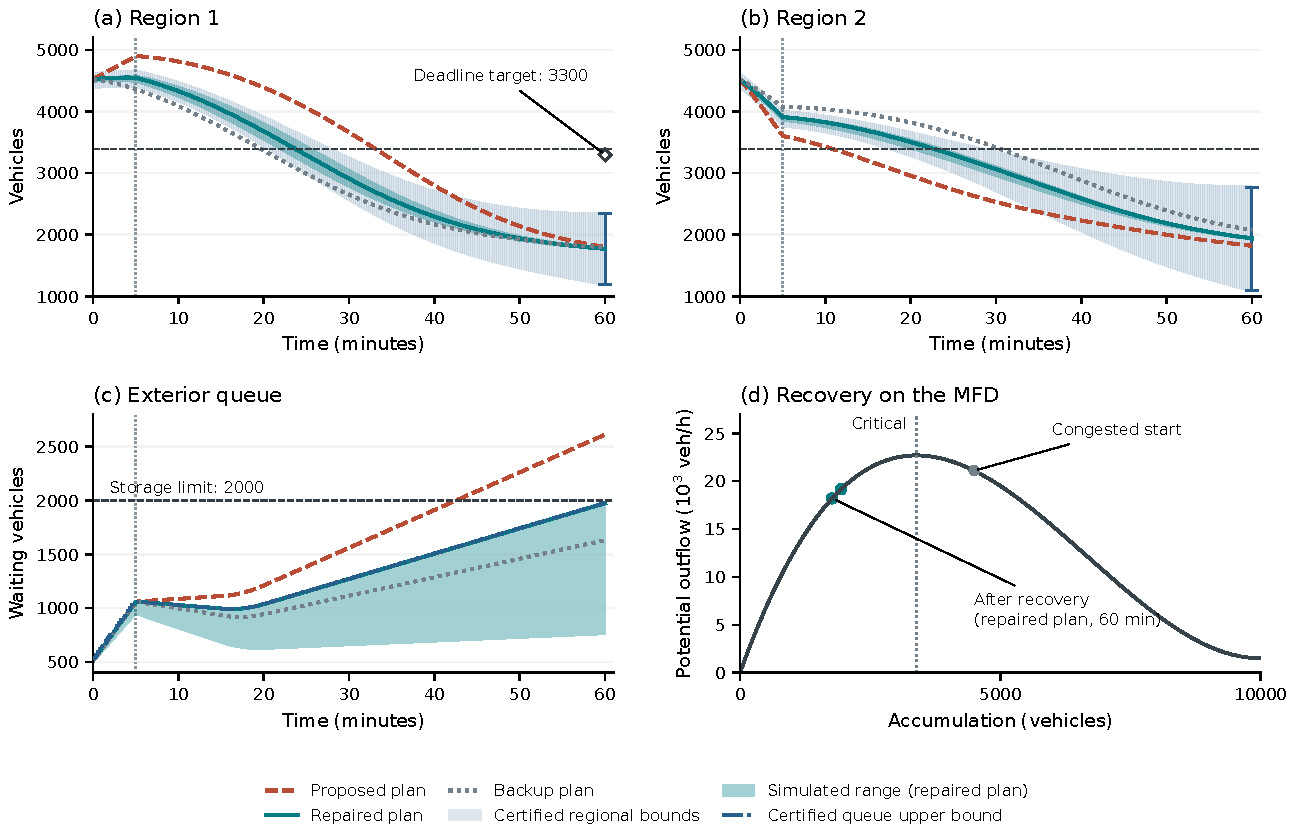
\includegraphics[width=0.96\linewidth]{figures/congested_recovery_compact_2026_11_16.pdf}
\caption{Recovery from congestion under proposed, repaired and backup
plans. Panels (a)--(c) use the same initial state
$x(0)=\widehat x_0+d_x$, at the upper bounds of the estimation box,
and arrivals 600~veh/h above forecast. Dark shading shows the range
of 640 simulations under repair. Light shading in (a)--(b) gives
certified regional bounds, with endpoint bounds shown by the bars at
minute~60. The blue dash-dot curve in (c) is the certified queue upper
bound. Horizontal dashed lines mark critical accumulation in
(a)--(b) and queue capacity in (c); the diamond marks the Region-1
deadline target. Each plan starts at minute~0; vertical dotted lines
at minute~5 mark its scheduled control switch. Panel~(d) places the
initial estimate and the repaired plan's two final regional
accumulations on the MFD. The unchecked trajectory continues after
queue overflow; spatial spillback is not modeled.}
\label{fig:congested-counts}
\label{fig:verification-enclosure}
\end{figure}

The selected repair has $\lambda_{\rm rep}=0.65$. An exact queue
balance demonstrates overflow for every smaller tested weight
(\appref{app:congested-diagnostics}). The destination-coordinate check
certifies the backup and repair throughout the hour, with
capacity-limited admission. For repair, the certified queue maximum is
below 1974 vehicles and the minute-60 regional upper bounds are 2342
and 2772 vehicles, rounded upward. Both regions therefore finish below
critical accumulation for every allowed initial state and arrival
error. Table~\ref{tab:congested-results} reports the traffic outcomes.
\begin{table}[pos=!htb]
\centering\small
\caption{Congested recovery over 640 matched simulations. TTS includes
both regions and the exterior queue; $J_D$ weights Region~2 by $p=4$.
Costs are medians in veh-h, maximum queue is in vehicles, and ``Meeting
both requirements'' counts simulations satisfying all physical
constraints and the service deadline. Certification covers the full
uncertainty set; the proposal's violation also follows from an exact
queue balance.}
\label{tab:congested-results}
\begin{tabularx}{\linewidth}{@{}Xrrr@{}}
\toprule
Measure & Proposed & Repaired & Backup\\
\midrule
Median TTS (veh-h) & 7495.1 & 7098.6 & 7018.8\\
Median $J_D$ (veh-h) & 15507.6 & 16157.4 & 16796.6\\
Maximum queue (vehicles) & 2610.0 & 1973.4 & 1630.7\\
Meeting both requirements & 320/640 & 640/640 & 640/640\\
Full-hour outcome & Violation shown & Certified & Certified\\
\bottomrule
\end{tabularx}
\end{table}

Relative to backup, repair lowers median priority cost by 3.8\% at a
1.1\% increase in TTS, retaining 49.6\% of the proposal's median
priority benefit. The case starts at an outflow approximately 7.1\%
below capacity and uses a 25-vehicle initial bound, or 0.6\% of the
regional accumulation. The queue bound closely follows the simulated
range, while the regional bounds are visibly wider. Their effect on
acceptance is examined in \appref{sec:structure-results}.

\paragraph{Three-region recovery}
\label{sec:multi-region-results}
The second example starts with three congested regions connected in
the directed ring $1\to2\to3\to1$, each with an exterior entry queue.
The initial estimate has 4500 vehicles in each region and 500 in
each queue. Arrivals are forecast at 6000~veh/h per queue,
with a 30\% increase at Queue~1 over minutes 15--45. The initial
error bounds are $25/3$ vehicles per destination-specific accumulation
and 10 vehicles per queue, giving a regional-total error bound of
25 vehicles. Arrival errors are independently bounded by 300~veh/h
at each queue. Every region must contain at most 3300 vehicles at
minute~60, and each queue has capacity for 2000 vehicles.

A prescribed proposal gives Region~1 priority by reducing its entry
input from the backup value of 0.55 to 0.495 after minute~5. All plans
start at minute~0 with a five-minute entry closure that allows the
regions to discharge traffic before admissions resume. The remaining
inputs and model settings are given in \appref{app:network-transfer}.
Figure~\ref{fig:three-region-traffic} compares the proposal, backup
and repaired plan under the same allowed initial state and arrival
errors, pairing each region with its entry queue.

The proposal brings regional counts down but lets Queue~1 reach
2265 vehicles. Repair selects weight 0.45 on the interpolation grid,
raising the entry input to 0.51975 and admitting another 297~veh/h
after minute~5. The repaired plan has verified queue maxima below
1993, 1311 and 1311 vehicles, respectively. Its regional deadline
bounds are 2436, 2365 and 2328 vehicles, rounded upward, so all three
targets are met. The backup also passes the full-hour verification.
After admissions resume, the repaired plan keeps the Region-1
count below the backup in the illustrated simulation while respecting
all queue capacities. The plan curves for Queues~2 and~3 coincide because
their entry inputs and illustrated arrival conditions are unchanged.

Signed destination-coordinate bounds verify this recovery, using the
tighter Jacobian evaluation described in \appref{app:verified-arithmetic}.
The queue balance establishes overflow for every smaller repair weight
on the tested grid. \appref{app:network-transfer} provides this argument,
the matched-simulation settings and the supporting ring-network cases.

\begin{figure}[pos=!htb]
\centering
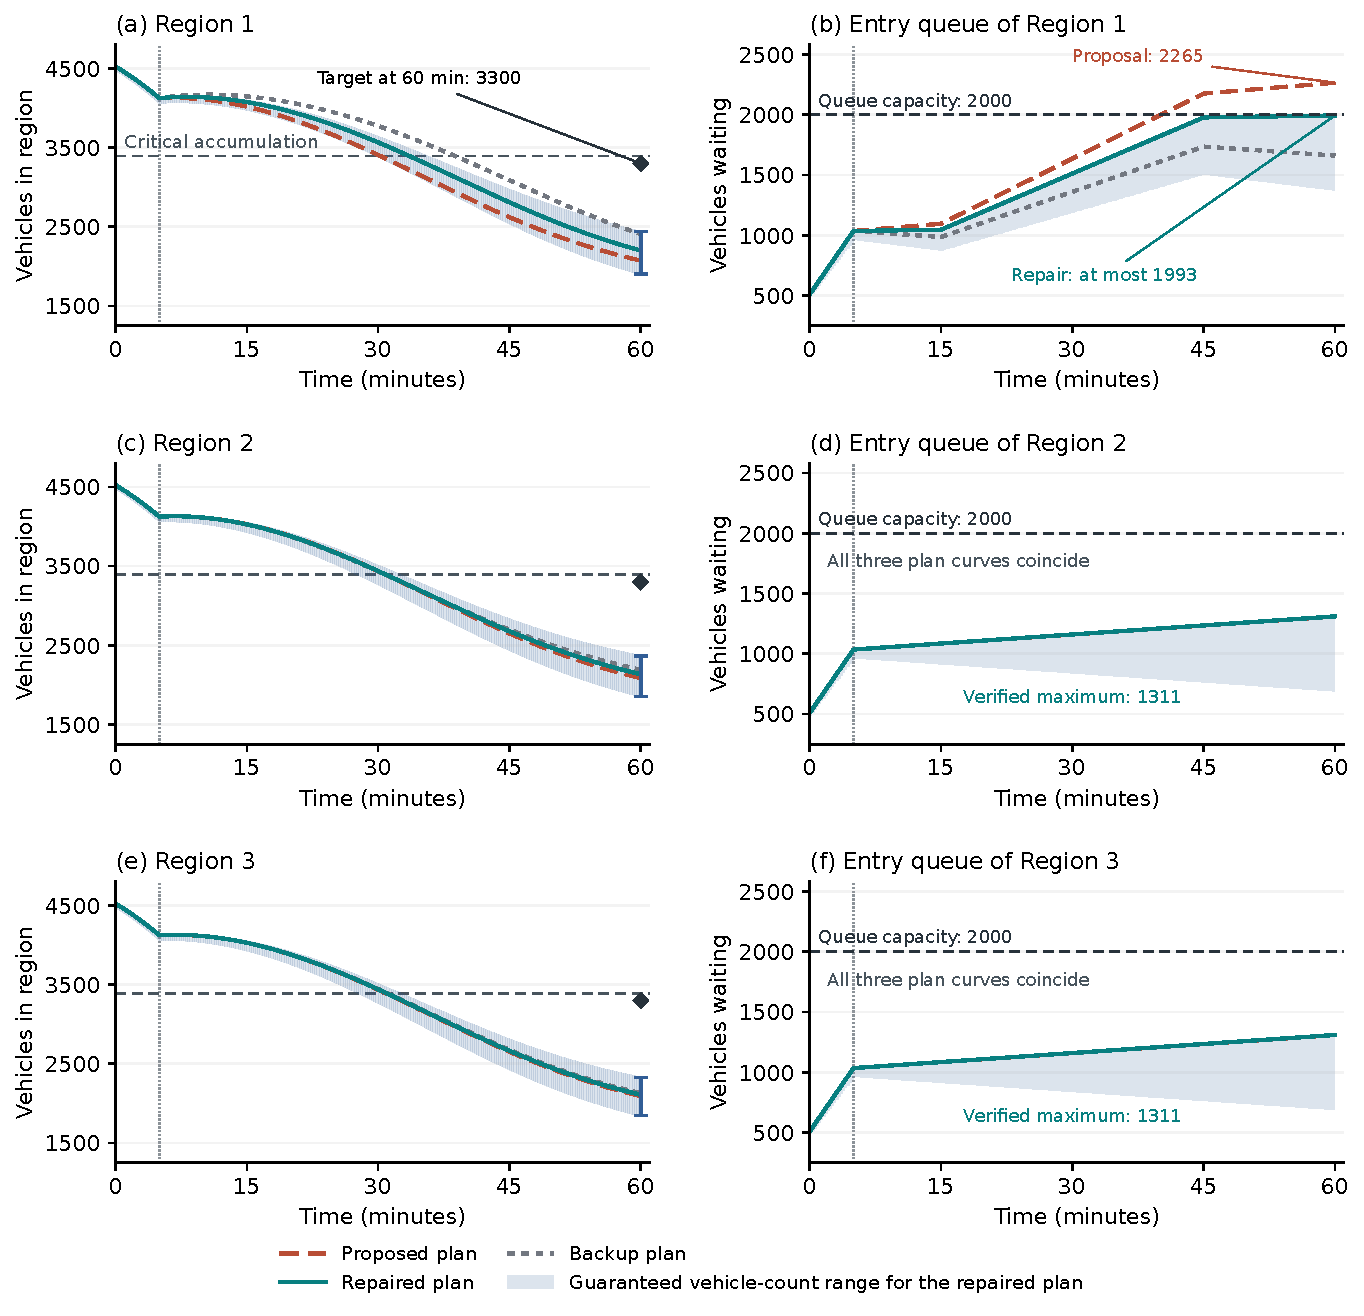
\includegraphics[width=\linewidth]{figures/three_region_recovery_all_queues_2026_11_16.pdf}
\caption{Congested recovery in three connected regions. Each row pairs
a regional vehicle count with its entry queue. All three plans use
the same allowed conditions: every destination-specific initial count
is $25/3$ vehicles above its estimate, each initial queue is 10 vehicles
above its estimate, and each arrival error is $+300$~veh/h. Shading gives
the guaranteed vehicle-count range for the repaired plan over all
allowed initial states and arrival-error signals. Diamonds mark the
3300-vehicle targets at minute~60; endpoint bars show the tighter
verified bounds at that time. Horizontal dashed lines indicate critical
accumulation in the left panels and queue capacity in the right panels.
Vertical dotted lines mark the scheduled input change at minute~5.
The three plan curves overlap in (d) and (f). The proposed trajectory
continues beyond overflow under the point-queue model. Displayed verified
maxima are rounded upward to whole vehicles.}
\label{fig:three-region-traffic}
\end{figure}

\subsection{Regional priority and service deadlines}
\label{sec:new-incident-protocol}
\label{sec:repair-results}

\paragraph{Increased arrivals and a tight regional deadline}
At minute~20, exterior arrivals have reached 7800~veh/h and the operator
requests Region-2 priority with $p=4$. This example uses
$d_x=\mathbf1_7$ vehicles, $\bar w=300$~veh/h and a Region-1 limit of
2850 vehicles at minute~60. Repair changes traffic movements to
relieve the queue and meet the regional deadline. In the upper-corner,
high-arrival simulation, it increases admission at minute~25 from 4594 to
5447~veh/h and the transfer input $u_{12}$ from 0.397 to 0.548.
The larger admission relieves the queue, while the increased transfer
from Region~1 helps meet its deadline. Figure~\ref{fig:traffic-snapshots}
in \appref{app:additional-numerics} shows the corresponding vehicle
counts and flows at minutes 20, 40 and 60.

Table~\ref{tab:benchmark-conflict} extends this comparison to all 640
matched simulations. The current plan is the plan already in force
when the regional-priority request arrives at minute~20. This
comparator continues its remaining control schedule unchanged,
rechecked against the same uncertainty bounds and deadline.
Nominal MPC gives the lowest median priority cost
but violates requirements in part of the set. CBF-QP keeps the physical
constraints satisfied in every simulation. It misses the regional
deadline in all of them; that requirement is outside its formulation.
This comparison shows the additional service
requirement addressed by the supervisor.
Repair meets both requirements and has a continuous certified queue
bound of 1682.7 vehicles. Continuing the current plan produces the
lowest TTS but the highest priority cost. Among the certified options,
repair therefore gives greater effect to the requested regional priority.

\begin{table}[pos=!htb]
\centering\small
\caption{Regional-priority comparison over 640 matched simulations per
strategy, minutes 20--60. TTS and $J_D$ ($p=4$) are median costs in
veh-h. Peak queue and $n_1(E)$ are maxima across the simulations, in
vehicles, with limits 2000 and 2850, respectively. ``Both met'' counts
simulations meeting all physical constraints and the deadline. The
last column distinguishes full-set verification from violations
found in simulation. The current plan continues the control schedule
already in force at minute~20. Queue maxima are rounded to one
decimal place; costs and deadline counts are rounded to whole units.
MPC is model predictive control; CBF-QP is the feedback quadratic
program enforcing physical constraints. Its deadline is an evaluation
criterion and is not included in the QP.}
\label{tab:benchmark-conflict}
\setlength{\tabcolsep}{3pt}
\begin{tabularx}{\linewidth}{@{}>{\raggedright\arraybackslash}p{3.4cm}rrrrr>{\raggedright\arraybackslash}X@{}}
\toprule
Strategy & TTS & $J_D$ & \shortstack{Peak\\queue} & $n_1(E)$ & \shortstack{Both\\met} & Check outcome\\
\midrule
Nominal MPC & 3241 & 6264 & 2180.0 & 2853 & 168/640 & Violation shown\\
CBF-QP & 3238 & 6293 & 1843.8 & 2918 & 0/640 & Physical limits met; deadline missed\\
Current plan & 2649 & 6714 & 194.4 & 1728 & 640/640 & Certified\\
Repaired plan & 3037 & 6363 & 1682.7 & 2311 & 640/640 & Certified\\
\bottomrule
\end{tabularx}
\end{table}

\paragraph{Larger state-estimation errors}
The same nominal proposal and backup also admit a certified repair with
$d_x=25\mathbf1_7$ vehicles, retaining $p=4$, $\bar w=300$~veh/h and
the 2850-vehicle deadline. Table~\ref{tab:repair-error-comparison}
compares the two cases. The selected repair places greater weight on
backup for the larger error bound, while its deadline bound remains below the
target. These are tested error bounds and require calibration for a
particular network.
\begin{table}[pos=!htb]
\centering\small
\caption{Repaired plans for the same regional-priority request under
different componentwise state-error bounds $d_x=d\mathbf1_7$. The
proposal, backup, arrival-error bound of 300~veh/h, priority weight
$p=4$ and minute-60 deadline of 2850 vehicles are unchanged.
The certified deadline upper bound is rounded upward; maximum queue
is taken over 640 simulations and rounded to one decimal place.
Both plans satisfy physical and service requirements in all 640
simulations and have full-interval certificates.}
\label{tab:repair-error-comparison}
\begin{tabularx}{\linewidth}{@{}Xrrr@{}}
\toprule
\shortstack{Error bound $d$\\(vehicles)} &
\shortstack{Repair weight\\$\lambda_{\rm rep}$} &
\shortstack{Certified deadline\\upper bound (vehicles)} &
\shortstack{Maximum simulated\\queue (vehicles)}\\
\midrule
1 & 0.25 & 2814 & 1682.7\\
25 & 0.30 & 2833 & 1583.4\\
\bottomrule
\end{tabularx}
\end{table}

\paragraph{Traffic costs across regional-priority scenarios}
Across the 80 uncertainty, priority and deadline settings detailed in
\appref{sec:uncertainty-results}, 36 nominal proposals pass unchanged
and 38 are repaired. Table~\ref{tab:repair-traffic-tradeoffs} shows the
paired traffic effects over the $38\times640=24{,}320$ repair simulations.
The median priority-cost reduction is 5.7\%, with a 16.1\% TTS increase
relative to backup and 91.7\% of the requested priority benefit
recovered. The priority objective represents an operator-selected
preference for Region~2, so improving it may increase network-wide
total time spent. Physical limits and service deadlines remain binding.
\begin{table}[pos=!htb]
\centering\small
\caption{Traffic effects of 38 repaired plans over 24,320 matched
simulations. Changes are relative to the corresponding backup. Benefit
retained is $100B_\omega$, relative to the proposed priority improvement.
All entries are percentages. Percentiles describe the prescribed
simulation set, not a probability model for traffic uncertainty.}
\label{tab:repair-traffic-tradeoffs}
\begin{tabularx}{\linewidth}{@{}Xrr@{}}
\toprule
Traffic measure & Median & 5th--95th percentiles\\
\midrule
Priority-cost reduction & 5.7 & 3.3--6.5\\
TTS increase & 16.1 & 7.8--21.4\\
Requested priority benefit retained & 91.7 & 56.8--96.2\\
\bottomrule
\end{tabularx}
\end{table}

The remaining six scenarios require newly certified backups, giving
an executable certified plan in all 80 tested settings. This availability
depends on obtaining a backup for the applicable specification, as
required by Lemma~\ref{thm:repair-grid}. Detailed acceptance counts are
given in Table~\ref{tab:repair-outcomes}.

For unchanged full-scenario MPC proposals, the requested priority
strongly affects acceptance. All tested proposals with $p=2$ or $p=3$
are verified, including the largest tested uncertainty bounds for
$p=2$. Only six of the 36 proposals with $p=4$ pass. The remaining
30 have a sampled Region-1 deadline margin of approximately one
vehicle, and the computed regional bounds cannot establish that
requirement. \appref{sec:uncertainty-results} gives the full comparison.

\subsection{Supporting studies}
\label{sec:supporting-studies}

\appref{app:additional-numerics} presents the supporting traffic and
agent studies. Successive-request tests show how the supervisory agent
accepts a beneficial replacement and retains the current plan after a
request that would cause queue overflow. Delayed-implementation tests
examine whether a replacement can be completed and verified from the
traffic conditions at its scheduled start. The agent experiments compare
interpretation with and without an explicit task record, while checking
the same physical constraints and service requirements. The appendix
provides the trajectories, outcomes and sensitivity to priority weights
and uncertainty bounds, together with the model-error tests and the
separate network-efficiency comparison.

\appref{app:bound-comparisons} compares verification methods for a fixed
control plan and reports the resulting traffic-state bounds and
computation times. Preserving shared uncertainty effects verifies a wider
tested range of initial-state errors than the interval comparisons,
although regional bounds remain wider than the simulated spreads.
\appref{app:experimental-settings} collects the experimental settings
and method definitions. These supporting studies describe the conditions
under which a proposal can pass unchanged, requires repair, or leaves the
current plan in use.

\section{Discussion and Implementation Requirements}
\label{sec:new-discussion}
\label{sec:information-model-scope}

The experiments show that serving a regional priority requires
balancing congestion inside the regions against waiting at the
boundary and traffic targets at fixed deadlines. Moderate-priority
full-scenario proposals are verified throughout the tested uncertainty
range, whereas stronger priorities often leave too little margin at
the Region-1 deadline for the computed bounds to establish satisfaction.
Thus a plan can meet every sampled traffic realization and still require
modification before its requirements are guaranteed over the full
uncertainty set. Repair retains part of the requested priority benefit;
its effect on network-wide TTS depends on the plan and traffic conditions.
The agent study concerns
objective selection: task records improve interpretation in the tested
histories, while the supervisor checks traffic limits and service
requirements independently of that selection.

Computation time affects both when a plan is ready and the traffic state
from which it starts. Delaying the plan start can allow a check to finish,
but leaves less time to meet pending deadlines. State propagation,
planning, checking and actuation must finish in time for the replacement
to start before the current plan ends. Measured check times depend on
the plan, uncertainty and implementation, so acceptance requires actual
completion by the plan start time.

The numerical certificates are conditional on a literature MFD, synthetic
internal demands, known event means, and the specified state and
arrival-error bounds. These bounds
require field calibration, particularly for the one-vehicle cases. The
two- and three-region congestion cases demonstrate full-hour recovery
with capacity-limited admission and substantial margins below their
regional deadline limits. Their regional bounds remain wider than the
sampled spreads.
The separate plant-sensitivity study shows why model error also matters:
combined adverse changes in MFD outflow and internal demand cause some
repaired trajectories to miss the deadline
(\appref{sec:plant-sensitivity-results}). The connected-ring examples
verify plans for networks with two and three entry queues under their
specified routing assumptions (\appref{app:network-transfer}).

Regional totals do not determine how many vehicles have each destination,
so deployment requires a joint estimate set for destination-specific
accumulations and queues, including measurement bias and timing errors.
Destination decomposition is also treated as uncertain in robust perimeter
control \cite{haddad2015robust}. Additional model error or feedback from
estimated states requires validated bounds on its effect during execution.
If a fresh estimate set is disjoint from the current certificate's reachable
set, the containment assumptions are inconsistent and recovery requires a
separate procedure. Operation beyond a finite plan additionally requires
the invariant policy, terminal-set inclusion and service coverage in
\appref{sec:terminal-backup}, with sustained arrivals compatible with
storage and discharge. Deployment therefore starts with a joint state
estimate, calibrated uncertainty bounds and a certified initial plan,
all consistent with the model and service requirements used by the checks.

\section{Conclusions}
\label{sec:new-conclusion}

This paper develops a dual-agent framework for urban perimeter control
in which an AI agent proposes plans and a rule-based supervisory agent
verifies them before implementation. Under the stated traffic and
interface assumptions, accepted plans satisfy physical constraints and
service requirements for all initial states and arrival errors within
the supplied bounds. The framework uses traffic structure to bound
future accumulations and queues, and preserves these guarantees through
plan replacement, repair and rejection, with additional conditions for
operation beyond a finite plan. The congested two- and three-region
cases show that a verified repair can bring regional counts below critical
accumulation while keeping all exterior queues within capacity. The comparative studies show how
repair retains part of a requested regional-priority benefit, with a
trade-off in total time spent, and how supervised replanning accommodates
changing requests and computation delays. They also show that strong
priorities can leave little margin before a service deadline, making
acceptance sensitive to the tightness of the regional bounds. In the
agent experiments, traffic requirements remain satisfied even when
the requested objective is misinterpreted.

Future work will develop joint estimates of regional destination-specific accumulations
and queues, calibrate their uncertainty bounds, and account for estimation
errors in feedback execution. Tighter regional bounds and planning
with sufficient constraint margins may improve acceptance without
repair. Further studies will address discrepancies between the model
and observed traffic, broaden congested-operation
tests to larger uncertainty sets and repeated estimation updates, and
evaluate larger sets of agent models and operator histories. Another
direction is to choose plan start times jointly with the plan, accounting
for sensing, computation, actuation and pending service deadlines.

\section*{Author contributions (Contributor Roles Taxonomy, CRediT)}
\textbf{Ali Eslami:} Conceptualization, Methodology, Software, Validation,
Formal analysis, Investigation, Data curation, Visualization,
Writing and editing.
\textbf{Jiangbo Yu:} Supervision, Review and editing.

\section*{Funding}
This research received no specific funding.

\section*{Declaration of generative AI and AI-assisted technologies in the manuscript preparation process}
ChatGPT, Claude and Codex were used to help restructure the manuscript
and improve the presentation of results. The authors reviewed and
edited the content and take full responsibility for the final manuscript.

\section*{Declaration of competing interests}
The authors declare that they have no known competing financial interests or
personal relationships that could have appeared to influence the work
reported in this paper.

\section*{Data and code availability}
Reproducibility materials include the traffic models, planning and
verification implementations, experiment protocols, stored agent requests
and responses, certificate records, and simulation outputs described in the
experimental settings in \appref{app:experimental-settings}. The materials are maintained at
\url{https://github.com/AlienEslami/agentic-perimeter-runtime-certification}.


\appendix
% Reset equations within each appendix and use appendix-letter labels.
\numberwithin{equation}{section}
\renewcommand{\theequation}{\Alph{section}.\arabic{equation}}
\numberwithin{table}{section}
\renewcommand{\thetable}{\Alph{section}.\arabic{table}}
\numberwithin{figure}{section}
\renewcommand{\thefigure}{\Alph{section}.\arabic{figure}}
\section{Notation}
\label{app:notation}

Table~\ref{tab:nomenclature} groups the notation by its role. Subscripts
identify regions, destinations, queues, state components, control blocks,
verification intervals or decisions according to context. Indexed forms
of the same quantity share the definition given here. The table collects recurring quantities. Symbols used only in a local
argument are defined beside their equations or in the corresponding proof.

\begingroup
\fontsize{9}{10}\selectfont
\renewcommand{\arraystretch}{1.03}
\setlength{\LTcapwidth}{\textwidth}
\begin{longtable}{@{}p{0.25\linewidth}>{\raggedright\arraybackslash}p{\dimexpr0.75\linewidth-2\tabcolsep\relax}@{}}
\caption{Notation used in the model, supervisory interface, verification,
experiments and appendices. Vehicle counts and queue lengths are in
vehicles, flow rates in veh/h, and time in hours unless stated otherwise.}
\label{tab:nomenclature}\\
\toprule
Symbol & Meaning\\
\midrule
\endfirsthead
\multicolumn{2}{@{}l@{}}{Table~\thetable\ (continued)}\\
\toprule
Symbol & Meaning\\
\midrule
\endhead
\midrule
\endfoot
\bottomrule
\endlastfoot
\multicolumn{2}{@{}l@{}}{\textbf{Traffic network, vehicle counts, and flows}}\\*
$N$, $n_q$, $n_{\rm acc}$ & Numbers of regions, exterior entry queues, and destination-specific vehicle-count variables; $n_{\rm acc}=|\mathcal A|$ (``acc'': accumulations).\\
$i,j,k,q$ & On traffic variables: current region $i$, final destination $j$, neighboring receiver $k$, and queue $q$. Destination or receiver $0$ denotes the exterior. Elsewhere these may be component or decision indices, as specified locally.\\
$\mathcal A$, $\mathcal E$ & Region--destination pairs $(i,j)$ included in the model; directed controlled boundaries $(i,k)$, including exterior exits.\\
$n_{ij}(t)$, $n_i(t)$ & Vehicles currently in region $i$ with final destination $j$; total vehicles in region $i$, $n_i=\sum_j n_{ij}$.\\
$c(t)$ & Vector of the $n_{ij}$ ordered by $\mathcal A$; for two regions, $(n_{11},n_{12},n_{10},n_{22},n_{21},n_{20})^\top$.\\
$z(t)$, $z_q(t)$ & Vector of exterior queue lengths in vehicles (scalar in the two-region model); number of vehicles waiting in queue $q$.\\
$x_{\rm net}$, $x$ & Network state $(c^\top,z^\top)^\top$; equivalent two-region coordinates $(n_1,n_2,n_{11},n_{22},n_{10},n_{20},z)^\top$.\\
$\mathcal L_i$, $\ell_i$ & Region-$i$ total lane length (lane-km); mean distance traveled within the region (km).\\
$\rho_i$, $V_i(\rho_i)$ & Regional density $n_i/\mathcal L_i$ (vehicles per lane-km); average speed at that density (km/h).\\
$G_i(n_i)$, $G(n)$ & Region-$i$ total potential outflow rate (veh/h), described by its MFD; common outflow curve used for both experimental regions.\\
$m_{ij}$, $m(c)$ & Potential outflow $n_{ij}V_i(n_i/\mathcal L_i)/\ell_i$, equal to $(n_{ij}/n_i)G_i(n_i)$ for $n_i>0$ and zero at $n_i=0$; vector of these rates ordered as $c$. For $j=i$ this is local trip completion.\\
$v_i(n)$, $v(n)$ & Per-vehicle potential outflow $G_i(n)/n$ (h$^{-1}$), with $v_i(0)=G_i'(0)$; common rate used in the experiments. These are rates, not speeds.\\
$n_i^{\rm crit}$, $n_i^{\max}$ & Vehicle count at a capacity maximum of region $i$'s outflow MFD; operational upper bound on its vehicle count.\\
$z_q^{\max}$, $z^{\max}$ & Storage limit of exterior queue $q$; single-queue storage limit in the two-region model (vehicles).\\
$d_{ij}^{\rm int}$, $d_i^{\rm int}$ & Rate of trips generated in region $i$ with destination $j$; total internal demand in that region, $\sum_j d_{ij}^{\rm int}$ (veh/h).\\
$d^{\rm int}(t)$ & Vector of internal demand rates $d_{ij}^{\rm int}(t)$ ordered as $c$.\\
$u$, $u_{ik}$ & Vector of boundary and entrance control inputs; fraction of assigned potential flow permitted from region $i$ to adjacent region $k$ ($k=0$: exterior). Each component lies in $[0,1]$.\\
$u_{12}$, $u_{21}$, $u_{20}$ & Two-region inputs controlling transfers $1\to2$, transfers $2\to1$, and departures $2\to0$. The input $u_{12}$ applies to both destination-2 and exterior-destination vehicles.\\
$u_q^{\rm in}$, $u_{02}$ & Fraction of full entrance capacity permitted for admission from queue $q$; single exterior entrance into Region~2. The two-region vector is $(u_{12},u_{21},u_{02},u_{20})^\top$.\\
$\mathsf R_{ik}^{(j)}$ & Fraction of potential destination-$j$ outflow from region $i$ assigned to boundary $(i,k)$ before control.\\
$B(u)$, $B_{:,ij}(u)$ & Matrix mapping potential outflows to vehicle-count changes through local completion, transfers and exterior exits; its column for pair $(i,j)$, defined in Section~\ref{app:new-model}.\\
$a(z,u)$, $a_q$ & Controlled admission rates from exterior queues into the network; rate from queue $q$ (veh/h). For one queue, $a=a(z,u_{02})$.\\
$\tau_q$, $\gamma_q^{\rm rel}$ & Queue-release time (h) and coefficient $\gamma_q^{\rm rel}=1/\tau_q$ (h$^{-1}$); $q=1$ in the two-region specialization.\\
$\kappa_q$, $\kappa_{02}$ & Full entrance capacity for queue $q$; single entrance capacity into Region~2 (veh/h).\\
$P_a$, $\pi$ & Admission-allocation matrix: column $q$ gives fractions assigned to receiving region--destination pairs; two-region fraction destined for Region~1, with $1-\pi$ destined for Region~2.\\
$\Lambda$, $\widehat\Lambda$, $w$ & Actual exterior arrivals, arrival forecast, and forecast error, with $\Lambda=\widehat\Lambda+w$ (veh/h); vectors for several queues. Subscript $q$ selects queue $q$.\\
$f_{\rm net}$, $B_w$ & Network dynamics using forecast arrivals; matrix $[0^\top,I_{n_q}]^\top$ inserting arrival errors into queue balances, with upper zero block of size $n_{\rm acc}\times n_q$.\\
$f(x,u,t)$, $f_b(x,t)$ & Two-region dynamics at zero arrival error; dynamics after substituting block law $u_b(x)=k_b+K_bx$. Actual dynamics are $f+e_7w$.\\
$F(c,u,t)$ & Regional balance term excluding admissions, $d^{\rm int}(t)+B(u)m(c)$.\\
$e_j$, $e_{ij}^{\rm acc}$ & Unit vector selecting state component $j$; unit vector for pair $(i,j)$ in $c$. For an exterior receiver, $e_{0j}^{\rm acc}=0$.\\
\addlinespace[3pt]
\multicolumn{2}{@{}l@{}}{\textbf{Plans, constraints, uncertainty, and objectives}}\\*
$P$, $[t_0,E]$ & Finite control plan and its execution interval, from start time $t_0$ to specified end time $E$.\\
$b$, $N_b$, $\tau_b$ & Control-block index $b=0,\ldots,N_b-1$, number of blocks, and block boundary times.\\
$k_b$, $K_b$, $u_b(x)$ & Input offset, state-feedback gain, and block law $u_b(x)=k_b+K_bx$. Constant-input plans have $K_b=0$.\\
$x_0$, $x_P$, $u_P$ & State at plan start; state trajectory and applied control under plan $P$, with initial state and arrival error specified as arguments.\\
$\mathcal U$ & Admissible control-input set, including component bounds and the two input-difference limits.\\
$\delta_1^u$, $\delta_2^u$ & Limits on $|u_{21}-u_{12}|$ and $|u_{20}-u_{02}|$, respectively.\\
$\mathcal P_{\rm phys}$ & Collection of physical state and control constraints.\\
$H_j$, $J_j$, $\beta_j^{\rm phys}$ & State and input coefficient rows and limit in physical constraint $j$: $H_jx+J_ju\le\beta_j^{\rm phys}$.\\
$n_c$, $n_s$ & Numbers of physical constraints and scheduled service requirements.\\
$r$, $T_r$, $g_r$, $\eta_r$ & Service-requirement index, deadline, state coefficient vector and vehicle-count limit: $g_r^\top x(T_r)\le\eta_r$. The vector radius $r_l$ has a separate meaning below.\\
$\mathcal O$, $\mathcal O_t$ & Service triples $(T_r,g_r,\eta_r)$ in the planning specification; accepted requirements still pending at time $t$.\\
$\widehat x_{t_0}$, $\widehat x_i$, $\widehat x_{t_a}$ & State estimate at initial plan start; estimate at decision $t_i$; predictor center or supplied estimate at delayed start $t_a$, as specified.\\
$\mathcal I_{t_0}$, $\mathcal I_t$, $\mathcal I_i$ & Sets containing all states allowed by the information used at initial start or time $t$; $\mathcal I_i=\mathcal I_{t_i}$.\\
$d_x$, $d_{x,k}$, $d_x(t_i)$ & Componentwise absolute state-error bounds, component $k$ of that vector, and bounds around the estimate or propagated center at decision $t_i$ (vehicles).\\
$d$, $\nu_i$ & Scalar parameter used to construct initial state-error bounds in experiments; estimation error $\widehat x_i-x(t_i)$, bounded by $d_x(t_i)$.\\
$\bar w$, $\mathcal W$, $\mathcal W_t$ & Absolute arrival-error bound (veh/h); allowed measurable error signals over the plan interval; corresponding remaining-time family at $t$.\\
$\mathcal C$, $\mathcal C(\mathcal S_t,E)$ & Planning specification $(\mathcal I_{t_0},\bar w,f,\mathcal P_{\rm phys},\mathcal O,[t_0,E])$; specification obtained from the decision record and candidate end time.\\
$\mathcal F_{\mathcal C}$, $\widehat{\mathcal F}_{\mathcal C}$ & Plans satisfying the specification for every allowed initial state and arrival error; subset accepted by verification.\\
$M$, $M_P$ & Total vehicles in both regions and the queue, $M=n_1+n_2+z$; this total along the trajectory under plan $P$.\\
$F_{\rm out}$ & Network departure rate $m_{11}+m_{22}+u_{20}m_{20}$, including local trip completion and exterior exits (veh/h).\\
$J_Q$, $J_D$, $p$ & Total-time-spent objective over $[t_0,E]$; corresponding regional-priority cost with Region~2 weighted by the dimensionless factor $p\ge1$ (both in veh-h).\\
$T_{\rm eval}$, $\mathrm{TTS}$ & Evaluation end time; total time spent in both regions and the queue over $[t_0,T_{\rm eval}]$ (veh-h).\\
$\omega=(x_0,w)$ & Matched realization: initial state and arrival-error signal used to compare plans.\\
$\Delta J_\omega$, $\Delta D_\omega$, $B_\omega$ & Repair's priority-cost reduction and TTS increase relative to backup (percent); fraction of the proposal's priority benefit recovered by repair.\\
\addlinespace[3pt]
\multicolumn{2}{@{}l@{}}{\textbf{Agent interface, replacement, and repair}}\\*
$\theta_i$, $T^{\rm prio}$, $D$ & Task record storing active and interrupted priorities; absolute priority end time; requested priority duration or extension in hours.\\
$\mathsf{Comp}$, $q_i^A$ & Request compiler that updates the task record; validated planning request containing priority, remaining duration and objective weights ($A$: agent request).\\
$\mathcal S_t$, $\mathcal S_t^{\rm rep}$ & Full decision record (state/error sets, requirements, current plan/certificate, backup, time and versions); its fields used for repair.\\
$\mathcal H_t$, $\mathsf{ver}_t$ & Current plan's certificate, including stored bounds; identifiers for model, forecast, physical-constraint and service-requirement versions.\\
$P_t^{\rm cur}$, $E_{\rm cur}$ & Plan currently in execution and its certified end time.\\
$P^0$, $P_i^0$ & Unmodified proposal, with $i$ indicating the decision when needed.\\
$P^B$, $P_t^B$, $P_i^B$, $E_B$ & Backup certified for the same specification as the repair candidates, optionally indexed by time or decision; its end time.\\
$\widehat P_i^R$, $P^R$ & Tool-returned repair candidate at decision $i$; selected certified repair used in performance comparisons.\\
$P^{\rm cand}$, $P_i^{\rm cand}$ & Replacement candidate, either an unmodified proposal or a repair.\\
$\mathsf{RepairTool}$ & Tool seeking a repair from proposal, backup, decision record and interpolation grid; every returned candidate requires verification.\\
$t_i^{\rm req}$, $t_i$, $t_a$, $t_{\rm ready}$ & Request time, decision/possible plan start time, delayed plan start time ($t_a=t_i$), and certificate-completion time; no completed result is represented by $t_{\rm ready}=\infty$.\\
$\mathcal R_P(t)$, $\mathcal R_{P,j}(t)$ & Certified reachable-state enclosure under $P$; enclosure from initial-cover member $j$. Their union is retained when the initial set is subdivided.\\
$P^{\rm exec}$, $u^{\rm exec}$ & Plan selected by the implementation rule; control input actually applied to the traffic system.\\
$\lambda_{\rm rep}$, $P(\lambda_{\rm rep})$ & Repair interpolation weight and candidate $(1-\lambda_{\rm rep})P^0+\lambda_{\rm rep}P^B$; weights $0$ and $1$ give proposal and backup.\\
$\mathcal G_{\rm rep}$, $\lambda_{{\rm rep},j}$, $N_{\rm rep}+1$ & Ordered repair-weight grid, its member $j$, and number of tested weights.\\
$\lambda_{\rm rep}^*$ & Smallest grid weight passing verification for the applicable decision record.\\
$\operatorname{dist}(P,P^0)$ & Chosen norm distance $\|P-P^0\|$ between stacked control-input vectors.\\
\addlinespace[3pt]
\multicolumn{2}{@{}l@{}}{\textbf{Coordinate transforms and verification bounds}}\\*
$y$, $y_c$, $L$ & Transformed state and its regional-coordinate block; under the allocation transform, $y_c=c+P_a z$ includes allocated queue shares. In the two-region analysis, $y=Lx$ and $L$ is invertible with the queue as its last coordinate.\\
$L_a$, $\widetilde L$ & Allocation transform $(c,z)\mapsto(c+P_a z,z)$; two-region transform $x\mapsto(c,z)$. Conservation coordinates use $L=L_a\widetilde L$.\\
$\mathsf{Cert}_t$, $\mathsf{Cert}^{\rm port}$ & Single-configuration and sequential portfolio verification procedures (port abbreviates portfolio). A completed check returns $1$ for verified satisfaction of the planning specification and $0$ when verification has not been established; $0$ alone does not prove a violation.\\
$\mathsf k$, $N_{\rm box}(\mathsf k)$ & Verification-configuration index and number of initial boxes in that configuration (written $N_{\rm box}$ for a selected configuration).\\
$l$, $t_l$, $h_l$, $s$ & Verification-interval index, absolute start, duration $t_{l+1}-t_l$, and local time $s\in[0,h_l]$. The index is omitted for single-interval arguments, giving $h=h_l$.\\
$\mathbf p_l$, $p_{il}$ & Physical-state predictor on interval $l$ and its component $i$, distinct from priority weight $p$.\\
$r_l$, $R_l$, $r_{il}$, $R_{il}$ & Initial and whole-interval candidate bounds on transformed error $L(x-\mathbf p_l)$; their component-$i$ values.\\
$a_{il}^{\rm cmp}$, $b_{ijl}^{\rm cmp}$ & Bounds on transformed Jacobian diagonal growth and off-diagonal coupling from component $j$ to $i$ (h$^{-1}$); ``cmp'': comparison.\\
$c_{il}^{\rm cmp}(R_l)$ & Bound on combined component coupling, predictor mismatch and arrival-error contributions (transformed-state units per hour).\\
$\delta_{il}$, $\epsilon_l$ & Componentwise bound on the transformed predictor derivative mismatch; residual $Lf_b(\mathbf p_l,t)-L\dot{\mathbf p}_l$.\\
$\phi_{il}(s)$, $\chi(\mu,s)$ & Componentwise comparison radius; integral $\int_0^s e^{\mu\tau}\,d\tau$ with scalar growth coefficient $\mu$.\\
$\xi$, $\Gamma_l$, $\zeta_l$ & Fixed normalized initial error with $|\xi|\le\mathbf1$, signed generator matrix and remainder in $L(x-\mathbf p_l)=\Gamma_l\xi+\zeta_l$.\\
$A_l^{\rm mv}$, $A_l^0$ & Transformed mean-value Jacobian and fixed reference matrix propagating the signed generators on interval $l$.\\
$\overline M$, $b_\zeta$, $\Psi(s)$ & Metzler comparison matrix for remainder growth, additive remainder-contribution bound, and matrix integral $\int_0^s e^{\overline M\tau}\,d\tau$.\\
$r_l^{\rm rem}$, $(r^{\rm rem})^+$ & Remainder bound at interval start; bound passed to the next interval (``rem'': remainder; $+$: successor interval).\\
\addlinespace[3pt]
\multicolumn{2}{@{}l@{}}{\textbf{Terminal continuation}}\\*
$\mathcal K$, $\mu_{\rm term}$ & Robustly invariant terminal set and feedback policy maintaining physical constraints within it beyond a finite plan's end.\\
$\mathsf{Cert}^{\mathcal K}_t$ & Plan verification augmented by terminal-set inclusion, pending-deadline coverage and an implementable transition to the terminal policy.\\
\addlinespace[3pt]
\end{longtable}
\endgroup


\section{Essential Experimental Settings}
\label{app:experimental-settings}
\label{app:reusable-benchmark}
\label{sec:supp-queue-settings}
\label{app:benchmark-details}

This appendix gives the settings supporting
Section~\ref{sec:new-evidence}. Table~\ref{tab:study-overview} collects
the traffic conditions, and Table~\ref{tab:verification-methods}
identifies the bounding methods. Exact stored states, plans and
execution instructions are provided in the reproduction materials
\cite{perimeterReproductionGuide}. The ring-network settings and
supporting results for Figure~\ref{fig:three-region-traffic} are in
\appref{app:network-transfer}.

\begin{table}[pos=!htb]
\centering\footnotesize
\caption{Settings of the numerical studies. State-error bounds $d_x$ and
deadline limits $\eta$ are in vehicles, and arrival-error bounds $\bar w$
are in veh/h. The congested, coordinate and ring studies cover minutes
0--60; the other studies cover minutes 20--60. For seven-state studies,
``regional/queue'' gives the bound on each of the first six components
and on the queue. The supporting-ring row lists the two- and
three-region cases in that order. Arrival error is bounded separately
at each queue. A dash denotes a prescribed plan without a specified
priority weight. The three-region recovery uses prescribed plans with
Region-1 priority.
For the tighter deadline, the controller comparison uses $d=1$;
the repaired-plan comparison also uses $d=25$.}
\label{tab:study-overview}
\setlength{\tabcolsep}{3pt}
\begin{tabularx}{\linewidth}{@{}>{\raggedright\arraybackslash}p{2.6cm}l>{\raggedright\arraybackslash}Xrrlr@{}}
\toprule
Study & Location & $d_x$ & $\bar w$ & $\eta$ & $p$ & Cases\\
\midrule
Congested recovery & \ref{sec:congested-results} & 25 regional, 10 queue & 600 & 3300 & 4 & 1\\
Coordinates and bounds & \ref{sec:structure-results} & $d=1$--$100$, queue $\min(d,10)$ & 60 & 2850 & 1 & 6\\
Proposals and repair & \ref{sec:new-incident-protocol}, \ref{sec:uncertainty-results} & $d\mathbf1_7$, $d=1$--$50$ & 60--300 & 2750--2950 & 2--4 & 80\\
Conservatism and computation & \ref{app:bound-comparisons} & 25 regional, 10 queue & 300 & 3300 & 4 & 2 plans\\
Three-region recovery & \ref{sec:multi-region-results} & $25/3$ per destination, 10 per queue & 300 & 3300 & 4 & 1\\
Supporting rings & \ref{app:network-transfer} & $25/N$ per destination, 10 per queue & 300/60 & 2700 & -- & 2\\
Tighter deadline & \ref{sec:new-incident-protocol} & $d\mathbf1_7$, $d=1,25$ & 300 & 2850 & 4 & 2\\
Plan replacement & \ref{sec:sequential-handover-results} & $\mathbf1_7$ initially & 300 & 2750 & $4,2,4$ & 1\\
Delayed activation & \ref{sec:sequential-handover-results} & $d\mathbf1_7$ initially, $d=1$--$50$ & 60--300 & 2750--2950 & $3,4$ & 17\\
Agent requests & \ref{sec:task-state-live} & $\mathbf1_7$ & 300 & 2850 & varies & 4 histories\\
\bottomrule
\end{tabularx}
\end{table}

\begin{table}[pos=!htb]
\centering\small
\caption{Bounding configurations used in the numerical comparisons.
Signed methods retain a common initial-error vector; interval methods
bound component errors separately. Initial-set subdivision, when used,
is stated separately.}
\label{tab:verification-methods}
\begin{tabularx}{\linewidth}{@{}l l X@{}}
\toprule
Method label & Coordinates & Bounds used\\
\midrule
State intervals & $x$ & Componentwise interval bounds\\
Destination intervals & $\widetilde Lx$ & Componentwise interval bounds\\
Conservation intervals & $Lx$ & Componentwise interval bounds\\
\shortstack[l]{Nonnegativity and\\queue bounds} & $Lx$ & Intervals with nonnegativity and independent queue bounds\\
Signed conservation & $Lx$ & Signed generators with nonnegativity and independent queue bounds\\
Signed destination & $\widetilde Lx$ & The same signed-generator construction in destination coordinates\\
\bottomrule
\end{tabularx}
\end{table}

\paragraph{MFD properties}
\label{app:mfd-properties}
Zhong et al.~\cite{zhong2018robust} give the cubic MFD in veh/s and
report a critical accumulation of 3400 vehicles, a maximum outflow of
6.3~veh/s, and a jam accumulation of 10,000 vehicles. The more precise
values in Section~\ref{sec:experimental-setup} are calculated from the
coefficients of that polynomial, after conversion to veh/h. In
particular,
\[
G'(n)=4.4631\times10^{-7}n^2-0.005963n+15.0912
\]
has roots near 3391.9308 and 9968.7378 vehicles. The first gives the
maximum outflow, approximately 22,691.2916~veh/h. The curve decreases
between the two roots, then rises slightly to
$G(10{,}000)=1532$~veh/h. Verification uses the polynomial and its
derivatives throughout the stated domain, including this final upturn.
The per-vehicle outflow rate nevertheless satisfies
\[
v'(n)=2.9754\times10^{-7}n-0.0029815<0,
\qquad 0\le n\le10{,}000.
\]
The associated speed therefore decreases over this domain for fixed
positive trip length, as in \eqref{eq:per-vehicle-outflow-rate}.

\paragraph{Implementation coordinates}
Stored calculations use 100 vehicles per unit, with
$\widetilde x=x/100$, $\widetilde w=w/100$ and
$\widetilde f(\widetilde x,u,t)=f(100\widetilde x,u,t)/100$.
Time and inputs are unchanged. State bounds and generators are
converted back to vehicles, and affine constraint thresholds are
scaled consistently. Reported counts and costs use physical units;
the reproduction guide gives the remaining conversion details.

\paragraph{Minute-20 state and plans}
For the studies initialized at minute 20 ($t_0=1/3$ h), the estimate
in the order of \eqref{eq:new-state} is approximately
\[
\widehat x_{t_0}=(2102.05,2315.67,1420.94,1487.71,240.28,301.84,124.11)^\top
\quad\text{vehicles}.
\]
The calculations use the full-precision state stored in the reproduction
materials. The current-plan comparator uses $(1,1,0.667015677,1)$ in control-input order
$(u_{12},\allowbreak u_{21},\allowbreak u_{02},\allowbreak u_{20})$, in five- and
35-minute blocks ending at minute 60. Its remaining schedule is rechecked for
each test case. If a new backup is needed, construction tries network TTS
followed by moderate Region-2 priority and certifies the result before
repair. The ordered repair grid is given in Section~\ref{sec:experimental-setup}.
Plans are converted to control-input coefficients and checked against exact
actuator constraints. State and service checks use 15-second verification subintervals.

\paragraph{Verification settings and test cases}
The scenario sets are defined in Section~\ref{sec:experimental-setup}.
The tighter-service-deadline, signed conservation plan-acceptance,
plan-replacement and agent-interpretation studies
use signed-generator propagation in conservation coordinates without initial-set
subdivision, with 15-second verification intervals. The structure study
compares the individual bounding methods. The fixed sequence of checks rechecks
160 nominal/full-scenario proposals and six structure settings. The
congested 600~veh/h result uses the destination-coordinate check
without subdivision, with the tighter interval-power evaluation and
iteration settings described in \appref{app:verified-arithmetic}. The matched 300~veh/h comparison additionally
evaluates four-box bounds and the computation time for the complete sequence of checks. The sequential procedure tests conservation coordinates without
subdivision, destination coordinates without subdivision, four-box
destination coordinates, and four-box conservation coordinates, in that
order. Subdivision bisects the initial ranges of $n_1$ and $n_2$ with
outward rounding. All four boxes must pass. Testing stops at the first
passing configuration, while a subdivided configuration stops at its
first failed box. Signed conservation repair searches retain their stated
verification configuration.

The 72 main-grid scenarios cross $d\in\{1,10,25,50\}$ vehicles,
$\bar w\in\{60,150,300\}$ veh/h, $\eta\in\{2750,2850,2950\}$ vehicles,
and $p\in\{2,4\}$. Eight validation cases use intermediate settings
$d\in\{5,20\}$, $\bar w\in\{100,225\}$,
$\eta\in\{2800,2900\}$, and $p=3$. Full-scenario MPC uses one-vehicle
prediction clearance with settings fixed across both sets.

Tables~\ref{tab:benchmark-deadlines} and \ref{tab:repair-outcomes}
in \appref{app:additional-numerics} report the unchanged-proposal and
repair counts. Results for the additional validation scenarios are
reported separately from the main grid, using the same fixed planner
and verification settings.





\paragraph{Trajectory simulations and comparisons}
OpenAI Codex assisted with implementation and plotting scripts.
Numerical figures are computed from the saved plans, simulation
outputs and certificate records using the supplied scripts.
For the two-region comparisons, simulations pair the five arrival-error
profiles defined above with all 128 initial-box corners, giving 640
simulations per plan. The control-Lyapunov-function (CLF) comparison
uses sixteen corners,
every eighth entry of the lexicographic $\{-1,+1\}^7$ list.
The minute-20 studies use fourth-order Runge--Kutta
(RK4) integration with ten-second steps. The congested 600~veh/h
comparison uses two-second steps, with unchanged compiled plans,
and 128 corners paired with the five arrival profiles. Both use independent
adaptive eighth-order Runge--Kutta (DOP853) integration and conservation
checks. CLF and CBF-QP comparators use exact simulated states at ten-second
updates, with constant control inputs between updates.
The CLF extension combines regional-error correction with
linear-quadratic admission/exit feedback and reference totals
$(2700,3200)$ vehicles. The CBF-QP minimizes deviation from
MPC subject to control-barrier-function inequalities for the physical constraints, with gain $6$ h$^{-1}$
and the worst queue-arrival error \cite{ames2017}. Its service deadline
is an evaluation criterion. 

For the matched comparison in Table~\ref{tab:benchmark-conflict},
the CBF-QP is evaluated on all 128 corners and five arrival profiles,
using the same gain, nominal plan and ten-second feedback updates as
the single-simulation comparison. All 640 simulations reach minute~60. Independent DOP853 integrations with maximum 2.5-second
steps retain the ten-second input updates for seven representative
or extremal cases. They preserve the physical-pass/deadline-fail
outcomes and change the reported costs and vehicle counts by less
than 0.1. No controller parameter is retuned.

\paragraph{Future activation}
\label{supp:detail:sec:delayed-handover-results}
\label{app:sequential-handover}
The seventeen delayed-activation cases comprise the eight extremes
$(d,\bar w,\eta,p)\in\{1,50\}\times\{60,300\}\times
\{2750,2950\}\times\{4\}$, tighter-service-deadline $(1,300,2850,4)$ case and eight
validation cases. The active plan supplies the activation box
$\mathcal I_{t_a}^+=\widehat x_{t_a}+[-d_x(t_a),d_x(t_a)]$, where
$(d_x(t_a))_i=\sum_j|(L^{-1})_{ij}|(r_{t_a})_j$, by outward conversion of its
endpoint enclosure obtained from signed-generator propagation. Here
$\widehat x_{t_a}$ is the corresponding predictor center, and
$r_{t_a}=|\Gamma(t_a)|\mathbf1+r^{\rm rem}(t_a)$ is the total
transformed error radius. This conversion preserves containment but can
lose dependence between state errors.
The recorded total computation time includes propagation,
optimization, checking and repair.



\paragraph{Agent interpretation experiments}
\label{app:agent-evaluation}
\label{sec:supp-execution}
\label{sec:queue-live-pilot}
\label{sec:primary-memory-pressure}
The live planning study in \appref{sec:task-state-live} pairs four
operator histories across history-only and task-record formats under
corrupted memory, giving eight interaction traces. Each trace contains
agent requests, tool responses and supervisory decisions. The agent uses
\texttt{gpt-5.4-mini-2026-03-17}, with reasoning disabled and prescribed
formats and arguments for tool requests. Each chosen objective leads to
a fresh MPC solve; following rejection, repair occurs only if the agent
requests it. The study uses thirteen live model queries and 640
simulations per executed schedule.

The four histories cover direct instruction, restoration after one or
nested interruptions, and an interrupted priority ending at minute 20.
The traffic setting is the tighter-service-deadline case in
Section~\ref{sec:new-incident-protocol}. Objectives set weights on
$(n_1,n_2,z)$ to $(1,1,1)$, $(4,1,1)$ or $(1,4,1)$ for network,
Region~1 or Region~2 priority. The separate stored-plan pilot and its
results are described in \appref{app:interpretation-pilot}.



\section{Numerical Implementation of the Verification Method}
\label{app:verified-arithmetic}

Acceptance bounds round coefficients, ranges, and comparison functions
outward: lower bounds downward and upper bounds upward, preserving all
allowed values. Generated predictors and trial radii support acceptance
only after these inequalities pass. For $K_b=0$, control-input constraints
are constant. Their stored binary coefficients are exact binary rationals,
so residuals, including zero, are checked exactly. State and storage
constraints still require verified trajectory bounds. This admits control inputs
on closed input boundaries without enlarging the control box.

Numerical evaluation of the matrix functions also needs verified error
bounds. Let $A$ be a matrix evaluated over a duration $h\ge0$.
The matrix norm $\|A\|_\infty$ is its maximum absolute row sum.
For a bound $\alpha\ge\|A\|_\infty$, the dimensionless product
$\sigma=\alpha h$, and Taylor-series truncation order $N_{\rm T}$,
\begin{equation}
 \begin{aligned}
 \left\|e^{Ah}-\sum_{k=0}^{N_{\rm T}}\frac{A^kh^k}{k!}\right\|_\infty
       &\le e^\sigma\frac{\sigma^{N_{\rm T}+1}}{(N_{\rm T}+1)!},\\
 \left\|\int_0^h e^{As}\,ds-
          \sum_{k=0}^{N_{\rm T}}\frac{A^kh^{k+1}}{(k+1)!}\right\|_\infty
       &\le he^\sigma\frac{\sigma^{N_{\rm T}+1}}{(N_{\rm T}+2)!}.
 \end{aligned}
 \label{eq:structure-matrix-tails}
\end{equation}
The norm exponential series gives the first bound. Integration with
$e^{\alpha s}\le e^{\alpha h}$ gives the second. Signed row coefficients
are formed before interval-time evaluation. Outward rounding covers every
coefficient, tail, product, sum, and generator conversion used in the
preceding tests. Equivalent scalar evaluation shortcuts and records of numerical
implementation checks are provided with the repository implementation.

The refined implementation uses the same acceptance inequalities with
tighter interval-power evaluation: an interval containing zero has a
nonnegative square, rather than the range obtained by multiplying two
independent copies. Batched matrix products retain the summation order
and outward rounding. A series order $N_{\rm T}=12$, with the explicit
tails in \eqref{eq:structure-matrix-tails}, replaces order 18. Trial
radii start with 1\% inflation and permit up to 64 iterations, replacing
10\% and 24 iterations. Failure to establish strict containment remains
inconclusive. These refinements change numerical enclosures and search
cost, while preserving the mathematical acceptance conditions.

For the three-region recovery, the Jacobian bounds use extrema of the
quadratic per-vehicle outflow rate. Each destination-specific Jacobian
entry depends on its own accumulation and the sum of the other
accumulations in that region. If both partial derivatives have fixed
signs throughout the trial box, its extrema occur at the corresponding
corners; otherwise outward interval evaluation is used. This tightens
the range without excluding any state from the box. This study uses
15-second intervals and series order 18, with 10\% initial trial-radius
inflation and up to 18 containment iterations. All interval bounds in
the accepted records were recomputed,
with additional high-precision checks of the Jacobian evaluation.

\label{app:bound-comparisons}
\paragraph{Effect of traffic-state bounds}
\label{sec:structure-results}
\label{sec:structure-online}

Figure~\ref{fig:coordinate-acceptance} holds the network-efficiency
plan fixed and changes only the method used to bound its trajectories.
Signed conservation bounds verify the tested regional initial-error
bound of 50 vehicles, while the passing interval methods reach
10 vehicles. The control inputs are identical in this comparison, so
the larger verified range comes from tighter bounds. The plan starts at
the reference equilibrium, with $\bar w=60$~veh/h, a 2850-vehicle
deadline target and queue error capped at 10 vehicles.

\begin{figure}[pos=htbp]
\centering
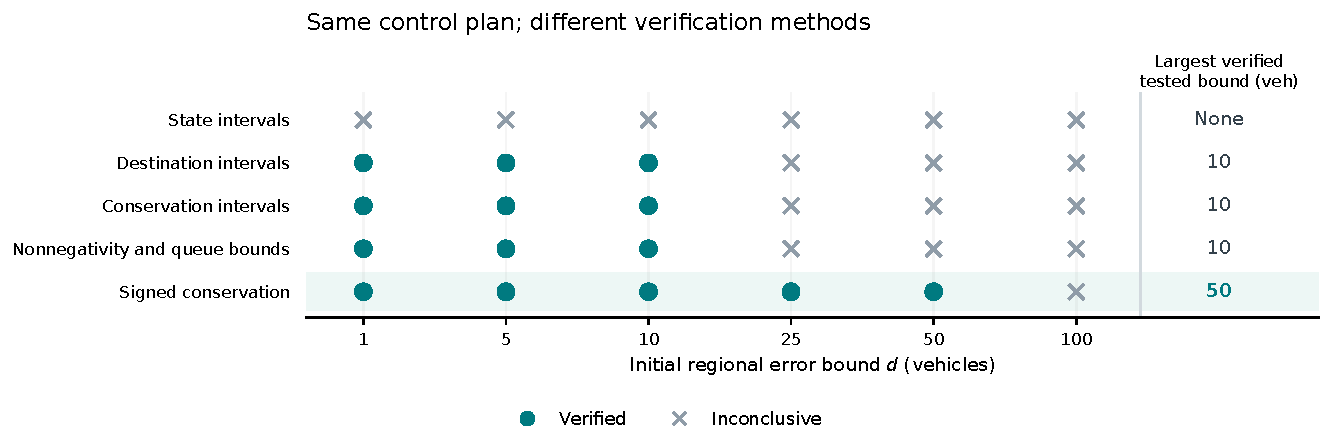
\includegraphics[width=\linewidth]{figures/coordinate_acceptance_2026_11_16.pdf}
\caption{Same control plan, different verification methods. The
network-efficiency plan and its control inputs are fixed. Circles
indicate complete verification and crosses indicate inconclusive checks
at the tested regional initial-error bounds $d$. The right column gives
the largest tested bound verified by each method; ``None'' means that
none of the displayed settings passes. Queue error is bounded by $\min(d,10)$ vehicles, arrival error by
60~veh/h, and Region~1 must contain at most 2850 vehicles at minute 60.
Signed conservation certifies $d=50$ vehicles, whereas the passing
interval methods reach $d=10$. An inconclusive check does not establish
a traffic violation. Figure~\ref{fig:structure-comparison} gives the
corresponding numerical upper bounds.}
\label{fig:coordinate-acceptance}
\end{figure}

\paragraph{Numerical bounds and computation times}
Figure~\ref{fig:structure-comparison} gives the numerical bounds for
the fixed-plan comparison above.
In the congested case of Section~\ref{sec:congested-results}, the
certified queue width equals the sampled width of 1220 vehicles,
comprising 20 from initial uncertainty and 1200 from arrival error
over the hour. Regional widths remain approximately 31--41 times
the sampled spreads.

A companion congested case uses the smaller arrival-error bound of
300~veh/h, the same backup, and a certified repaired plan with
$\lambda_{\rm rep}=0.35$. Table~\ref{tab:widths-times} compares
four-box regional widths and the time taken by the complete sequence
of checks. With the refined evaluation, this sequence takes
17.6--19.4 seconds over the recorded runs for these two plans,
including every attempted check but excluding planning, sensing and
actuation. The standard sequence reaches a four-box configuration,
whereas the refined evaluation accepts both plans without subdivision.
The times therefore include different stopping points and do not
provide a worst-case latency bound.

\begin{figure}[pos=htbp]
\centering
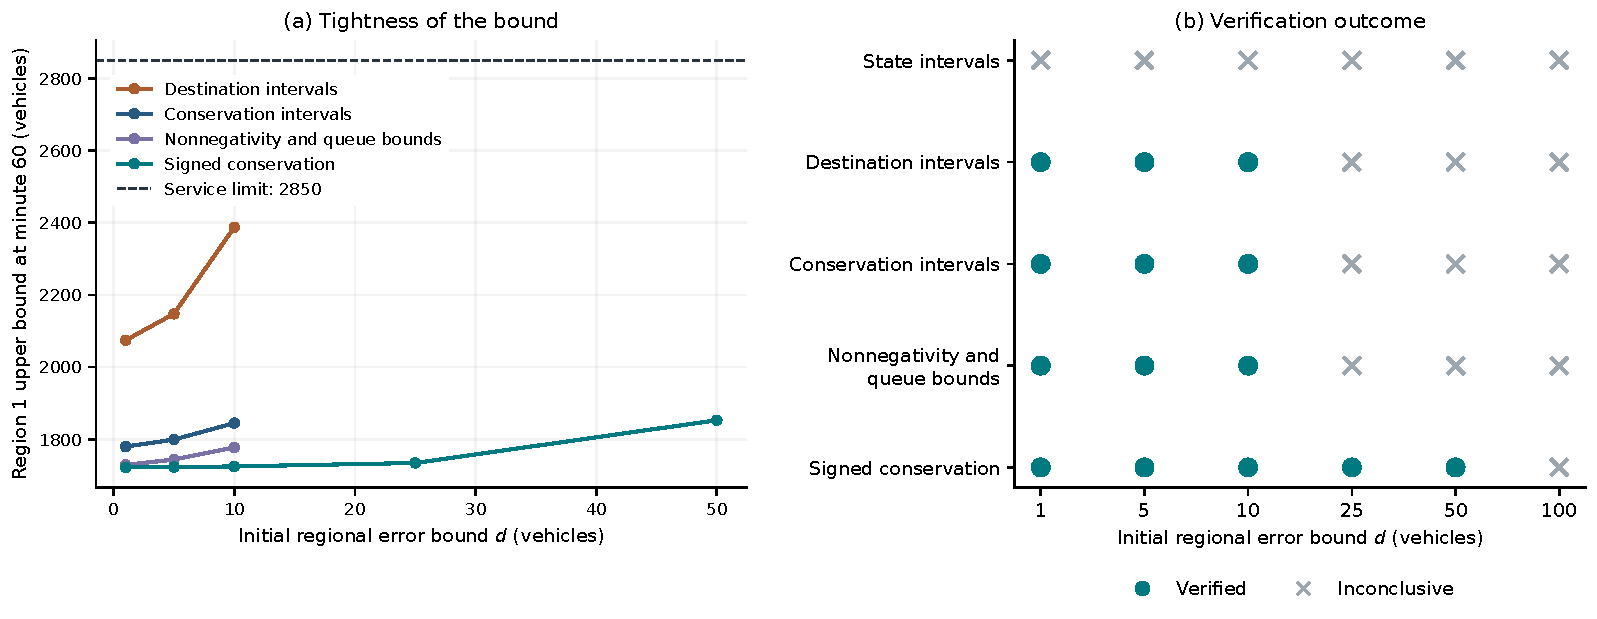
\includegraphics[width=\textwidth]{figures/structure_certification_comparison.pdf}
\caption{Verification of the same control plan as the initial regional
state-error bound $d$ increases, using the methods in
Table~\ref{tab:verification-methods}. (a) Certified upper bounds on the
number of Region-1 vehicles at minute 60; smaller values indicate tighter
upper bounds, and the service limit is 2850 vehicles. Values appear only when
the complete plan passes verification. (b) A circle means all physical
constraints and the service requirement are verified; a cross means the
check is inconclusive, not that the plan violates a constraint. Signed
conservation verifies this plan through $d=50$ vehicles, while the
passing interval methods reach $d=10$. Lines connect tested settings.
Queue error is bounded by $\min(d,10)$ vehicles and arrival error by
60~veh/h.}
\label{fig:structure-comparison}
\end{figure}

\begin{table}[pos=htbp]
\centering\small
\caption{Regional endpoint widths and acceptance times at
$\bar w=300$~veh/h for the congested backup and weight-0.35 repair.
Paired entries give Regions 1/2 at minute 60. Certified widths use the
four-box partition and are rounded upward to whole vehicles; sampled
spreads cover 640 simulations and are in vehicles. Ratios are certified
width divided by sampled spread, using unrounded data. Acceptance times
are ranges over two paired serial runs of the sequential procedure on
an Intel Core Ultra 7 255H, including unsuccessful checks and excluding
planning, sensing and actuation. The standard procedure stops after a
four-box check; the refined procedure stops at its unsplit check.}
\label{tab:widths-times}
\setlength{\tabcolsep}{4pt}
\begin{tabularx}{\linewidth}{@{}Xrrrr@{}}
\toprule
Plan / implementation & \shortstack{Certified\\widths} &
\shortstack{Sampled\\spreads} & Ratios & \shortstack{Acceptance\\time (s)}\\
\midrule
Backup, standard & 745/1208 & 28.1/67.0 & 26.5/18.0 & 70.4--78.1\\
Backup, refined & 494/793 & 28.1/67.0 & 17.6/11.8 & 18.9--19.3\\
Repair, standard & 692/894 & 58.3/41.8 & 11.9/21.4 & 77.1--77.7\\
Repair, refined & 486/609 & 58.3/41.8 & 8.3/14.6 & 17.6--19.4\\
\bottomrule
\end{tabularx}
\end{table}

\section{Task-Record Operations}
\label{app:task-operations}

The task record converts instructions into a current objective while
tracking interrupted priorities and their absolute end times. The complete
update rules are given in Table~\ref{tab:task-operations}. They affect the
objective requested from the planning tool without modifying the service
requirements maintained by the supervisor.

\begin{table}[pos=htbp]
\centering\small
\caption{Task-record operations. A duration $D$ is expressed here in
hours. Suspended priorities retain their original absolute end times.
Before each operation, an expired active priority is replaced by the
most recently interrupted unexpired priority, if one exists. With no
active priority, the objective is network efficiency. \appref{sec:supp-execution} specifies the operations exercised in
the agent histories.}
\label{tab:task-operations}
\begin{tabularx}{\textwidth}{@{}l>{\raggedright\arraybackslash}X>{\raggedright\arraybackslash}X@{}}
\toprule
Operation & Effect on $\theta_i$ & Resulting objective\\
\midrule
Set & Clear interrupted priorities and assign a new priority with
$T^{\rm prio}=t_i^{\rm req}+D$. & Newly requested regional objective.\\
Interrupt & Save the active priority, if any, then assign a temporary
priority with end time $t_i^{\rm req}+D$. & Temporary regional objective.\\
Continue & Keep the active record and its end time. & Current objective.\\
Extend & Add $D$ to the active end time. Reject if no active priority
remains. & Current regional objective.\\
Resume & Restore the latest unexpired interrupted priority. If none
survives, apply the rule below. & Restored regional objective or network
efficiency.\\
Cancel & Clear both the active and interrupted priorities. & Network
efficiency.\\
\bottomrule
\end{tabularx}
\par\smallskip\raggedright\footnotesize
For Resume, if no interrupted record exists and the active priority is
not temporary, that priority is preserved. Otherwise, if no interrupted
priority survives, the active priority is cleared. The accepted operation \texttt{network} has the same effect as Cancel.
An interruption is rejected when it would exceed the four-record stack
limit.
\end{table}

\section{Continuation Beyond Plan End Time}
\label{sec:terminal-backup-main}
\label{sec:terminal-backup}

The numerical studies evaluate finite plans and do not test the terminal
conditions in this appendix. A finite-plan certificate covers the execution interval ending at $E$.
Rejecting a replacement leaves this end time unchanged. Coverage beyond $E$
requires a replacement
activated by $E$ with a later certified end time or a certified terminal policy activated at $E$. If neither is available, the finite-plan result
establishes feasibility only through $E$.

In this framework, indefinite continuation uses a nonempty certified set
$\mathcal K$ and an implementable feedback policy $\mu_{\rm term}$. For every
state in $\mathcal K$ when that policy starts and every allowed uncertainty realization,
the terminal-policy trajectory exists for all future time, stays in $\mathcal K$,
and satisfies the physical state and input constraints. Policy
initialization is part of the certificate. The state-feedback policy
$\mu_{\rm term}(x)$ below assumes access to the exact values of the state components
on which it depends. An implementation using estimates requires its
measurement errors to be covered by the terminal certificate.

The following Lyapunov sublevel-set test \cite{khalil2002nonlinear}
provides sufficient conditions for a terminal policy. Applying it to the
queue-augmented model requires a verified policy, invariant set, and
service coverage. The control-Lyapunov-function (CLF) comparison in
\appref{sec:network-efficiency-comparison} is evaluated over finite plans and has
no such terminal certificate. In the test below, $g_{\rm term}$ is the
closed-loop vector field, $w_{\rm term}$ is its uncertainty input, and
$\mathcal W_{\rm term}$ contains the allowed uncertainty values. The
function $\mathcal V_{\rm term}$ defines the terminal set through its
level $\overline{\mathcal V}_{\rm term}$; $\lambda_{\rm term}$ is a
positive decay coefficient and $\bar d_{\rm term}$ bounds the additive
term in its derivative inequality. The subscript $\mathrm{term}$
identifies terminal-policy quantities.

\begin{proposition}
\label{prop:backup-lyapunov}
Suppose the implemented terminal policy has closed-loop dynamics
\[
\dot x=g_{\rm term}(x,w_{\rm term}),\qquad w_{\rm term}(t)\in\mathcal W_{\rm term},
\]
where $\mathcal W_{\rm term}$ is compact, $w_{\rm term}(\cdot)$ is measurable, and $g_{\rm term}$ is
continuous and locally Lipschitz in $x$, uniformly over
$w_{\rm term}\in\mathcal W_{\rm term}$, on an open domain $\Omega$. Let
$\mathcal V_{\rm term}:\Omega\rightarrow\mathbb R_{\ge0}$ be continuously differentiable and define
\[
\mathcal K=\{x\in\Omega:\mathcal V_{\rm term}(x)\le \overline{\mathcal V}_{\rm term}\},
\]
where $\mathcal K$ is nonempty and compact. If, on a neighborhood of
$\mathcal K$,
\[
\nabla \mathcal V_{\rm term}(x)^\top g_{\rm term}(x,w_{\rm term})
\le -\lambda_{\rm term} \mathcal V_{\rm term}(x)+\bar d_{\rm term}
\]
for all $w_{\rm term}\in\mathcal W_{\rm term}$, with
$\lambda_{\rm term}>0$ and
$0\le\bar d_{\rm term}\le\lambda_{\rm term} \overline{\mathcal V}_{\rm term}$, and if every state and input generated
on $\mathcal K$ satisfies the authorized physical constraints, then
$\mathcal K$ is robustly invariant under $\mu_{\rm term}$.
\end{proposition}

\begin{proof}
For a trajectory starting in $\mathcal K$ at $t_a$, the chain rule
and the assumed derivative bound give, almost everywhere in the stated
neighborhood,
$\frac{d}{dt}\mathcal V_{\rm term}(x(t))\le-\lambda_{\rm term} \mathcal V_{\rm term}(x(t))+\bar d_{\rm term}$.
An integrating factor yields
\[
 \mathcal V_{\rm term}(x(t))\le e^{-\lambda_{\rm term}(t-t_a)}\mathcal V_{\rm term}(x(t_a))+
 \frac{\bar d_{\rm term}}{\lambda_{\rm term}}\bigl(1-e^{-\lambda_{\rm term}(t-t_a)}\bigr)
 \le \overline{\mathcal V}_{\rm term}.
\]
The right-hand side is a weighted average of two quantities bounded by
$\overline{\mathcal V}_{\rm term}$. This comparison excludes departure from the sublevel set.
Compactness of $\mathcal K$ within the open domain, together with the
stated uniform local regularity, allows the solution to continue for
all future times. The physical constraints hold on $\mathcal K$ by
assumption, proving robust invariance under every allowed uncertainty.
\end{proof}

A plan activated at $t_i$ with end time $E_i>t_i$ is terminally certified
when it passes the physical and service checks on $[t_i,E_i]$, covers
every service requirement pending at activation, with all pending
deadlines included in that interval,
and its entire terminal reachable enclosure
$\mathcal R_i(E_i)=\mathcal R_{P_i}(E_i)$ satisfies
\begin{equation}
\mathcal R_i(E_i)\subseteq\mathcal K.
\label{eq:backup-terminal-landing}
\end{equation}
Its certificate specifies an implementable transition to $\mu_{\rm term}$ at
$E_i$, including required initialization. For
Proposition~\ref{prop:backup-lyapunov}, a sufficient test is
\begin{equation}
\sup_{x\in\mathcal R_i(E_i)}\mathcal V_{\rm term}(x)\le \overline{\mathcal V}_{\rm term}.
\label{eq:backup-computable-landing}
\end{equation}
Write $\mathsf{Cert}^{\mathcal K}_t$ for the verification procedure augmented with
these terminal conditions. Thus
\begin{equation}
\mathsf{Cert}^{\mathcal K}_t(P\mid\mathcal S_t)=1
\ \Longrightarrow\ \mathsf{Cert}_t(P\mid\mathcal S_t)=1.
\label{eq:terminal-checker}
\end{equation}
Acceptance additionally verifies terminal inclusion
\eqref{eq:backup-terminal-landing}, coverage of every pending deadline,
and an implementable transition to $\mu_{\rm term}$. Here the terminal enclosure
$\mathcal R_P(E_P)$ covers every trajectory in $\mathcal X_P$.

The following theorem carries this terminal guarantee through successive
replacements and activates the terminal policy when the active plan expires.
The actual plan start times $t_k^{\rm act}$ below are those decision times
$t_i$ at which a new plan starts, with $k$ counting these activations.

\begin{theorem}
\label{thm:backup-recursive-availability}
Let $\mu_{\rm term}$ be a certified terminal policy on $\mathcal K$. Enumerate
actual plan activations as $t_0^{\rm act}=t_0<t_1^{\rm act}<\cdots$,
with plans $P_k$ and end times $E_k$. Suppose
\[
\mathsf{Cert}^{\mathcal K}_{t_k^{\rm act}}
 (P_k\mid\mathcal S_{t_k^{\rm act}})=1,\qquad
x(t_k^{\rm act})\in\mathcal I_{t_k^{\rm act}},
\]
and suppose every activation preserves all pending service requirements.
Assume $\#\{k:t_k^{\rm act}\le T\}<\infty$ for every finite $T$, and
that execution and uncertainty satisfy the active certificate. Let $k(t)=\max\{k:t_k^{\rm act}\le t\}$, and suppose execution follows
\begin{equation}
u^{\rm exec}(t)=\begin{cases}
u_{P_{k(t)}}(t,x(t)),&t<E_{k(t)},\\
\mu_{\rm term}(x(t)),&t\ge E_{k(t)}.
\end{cases}
\label{eq:terminal-execution-policy}
\end{equation}
Suppose the certified policy initialization is applied at the plan's end time, and
a new service requirement during finite-plan execution becomes pending
only when the selected terminally certified plan covers its deadline.
During terminal-policy operation, a new requirement is accepted only
through a covering terminally certified plan. Then the trajectory exists
for every $t\ge t_0$, and
\begin{equation}
\begin{aligned}
H_jx(t)+J_ju^{\rm exec}(t)&\le\beta_j^{\rm phys},
 &&t\ge t_0,\\
g_r^\top x(T_r)&\le\eta_r,
 &&\text{accepted service requirements with }T_r\ge t_0.
\end{aligned}
\label{eq:terminal-global-guarantee}
\end{equation}
Rejection preserves the active plan and its terminal transition.
\end{theorem}

\begin{proof}
Each activated plan contains the actual state at plan start and is certified
for the allowed uncertainty. Theorem~\ref{thm:new-plan-closure} gives
its physical and service guarantees until replacement or the plan's end time.
If the next plan starts at or before $E_k$, its matching certificate
continues that guarantee. Otherwise,
\[
 x(E_k)\in\mathcal R_{P_k}(E_k)\subseteq\mathcal K,
 \qquad x(t)\in\mathcal K\quad(E_k\le t<t_{k+1}^{\rm act}),
\]
because the certified initialization activates $\mu_{\rm term}$ at the plan's end time.
Its invariant-set certificate covers that interval, indefinitely if
no further activation occurs. Rejection preserves this same terminal
transition. Only finitely many plans are activated in any finite
interval, so the certified plan and terminal-policy segments define
a solution for every $t\ge t_0$ and satisfy the physical constraints.

Every activated plan covers all pending service requirements
within its horizon, and replacements preserve that coverage. The rule
for accepting new requirements preserves this property between activations. At a
deadline, the covering certificate gives $g_r^\top x(T_r)\le\eta_r$.
By the plan's end time, all service deadlines assigned to that finite plan have been covered.
During terminal-policy operation, a new request is accepted only
through a covering terminally certified plan. Thus every accepted service
requirement is met, proving \eqref{eq:terminal-global-guarantee}.
\end{proof}

A service request made during terminal-policy operation is accepted
only after a new certificate covers that request and a terminal
continuation. A nonempty invariant set also requires arrivals compatible
with sustained discharge: finite exterior storage cannot accommodate
persistent allowed inflow above every attainable discharge rate. Any
diversion, upstream holding, or demand management used to meet this
condition must appear in the certified model.

The next corollary combines terminal continuation with ordered repair.

\begin{corollary}
\label{cor:repair-recursive}
Suppose repair uses the terminal verification procedure in
\eqref{eq:terminal-checker} with the decision record for actual
activation. Suppose also that
$\mathsf{Cert}^{\mathcal K}_t(P^B\mid\mathcal S_t)=1$ and
$1\in\mathcal G_{\rm rep}$. Then the terminally certified grid set
\begin{equation}
\mathcal G_{\rm rep}^{\mathcal K}(t)=
\{\lambda_{\rm rep}\in\mathcal G_{\rm rep}:
\mathsf{Cert}^{\mathcal K}_t(P(\lambda_{\rm rep})\mid\mathcal S_t)=1\}
\label{eq:repair-terminal-grid}
\end{equation}
is nonempty. Under the initialization, uncertainty, activation and
local-finiteness assumptions of
Theorem~\ref{thm:backup-recursive-availability}, activating only members
of this set and retaining the current plan on timeout preserves
\eqref{eq:terminal-global-guarantee}.
\end{corollary}

\begin{proof}
Since $P(1)=P^B$ and its terminal certificate passes,
$1\in\mathcal G_{\rm rep}^{\mathcal K}(t)$. Every selected grid
member has a certificate covering its finite physical and service
requirements and its terminal inclusion
$\mathcal R_{P(\lambda_{\rm rep})}(E_B)\subseteq\mathcal K$.
When all evaluations terminate, Lemma~\ref{thm:repair-grid} also gives
the least passing weight. Timeout retains the current terminal
certificate, schedule, and end time. Successful repair and continuation of the current plan
therefore both satisfy Theorem~\ref{thm:backup-recursive-availability},
which proves the stated continuation guarantee.
\end{proof}

\section{Traffic Cost of Plan Repair}
\label{sec:repair-cost-bound}
\label{app:repair-cost}

Repair changes the requested control inputs and can therefore change the
traffic objective. To relate these two changes, consider two piecewise-constant
plans with the same initial state and arrival error on $[t,t+T_{\rm cost}]$.
Use the Euclidean norm for control inputs, and a fixed norm for states.
Suppose both trajectories remain in one compact
domain on which, uniformly in time,
\[
\|f(x,u,s)-f(x^{\prime},u^{\prime},s)\|
\le L_x\|x-x^{\prime}\|+L_u\|u-u^{\prime}\|.
\]
Here $L_x$ and $L_u$ are nonnegative Lipschitz constants for changes
in state and control, respectively. For a common running cost
$j_{\rm run}$ and terminal cost $j_{\rm end}$, assume
$|j_{\rm run}(x,u)-j_{\rm run}(x^{\prime},u^{\prime})|\le L_{\rm run,x}\|x-x^{\prime}\|+
L_{\rm run,u}\|u-u^{\prime}\|$ and $|j_{\rm end}(x)-j_{\rm end}(x^{\prime})|\le L_{\rm end}\|x-x^{\prime}\|$.
The nonnegative constants $L_{\rm run,x}$ and $L_{\rm run,u}$ bound
running-cost sensitivity to state and control; $L_{\rm end}$ bounds
terminal-cost sensitivity to state. The positive duration $T_{\rm cost}$
is the cost-evaluation horizon. Set
$J(P)=\int_t^{t+T_{\rm cost}}j_{\rm run}(x_P,u_P)\,ds+j_{\rm end}(x_P(t+T_{\rm cost}))$.

The following proposition bounds the cost change caused by interpolation
toward the certified backup. The bound follows from the standard
Gronwall comparison for two trajectories under different controls
\cite{khalil2002nonlinear}.

\begin{proposition}
\label{prop:repair-cost}
Under these assumptions, for the Euclidean norm on the stacked fixed-block
control-input vector,
\begin{equation}
|J(P(\lambda_{\rm rep}))-J(P^0)|
\le L_J\lambda_{\rm rep}\|P^B-P^0\|_2,
\label{eq:repair-cost-bound}
\end{equation}
where
\begin{align*}
L_J&=L_{\rm run,x}L_u B_{T_{\rm cost}}+L_{\rm run,u}T_{\rm cost}+L_{\rm end}L_u A_{T_{\rm cost}},\\
A_{T_{\rm cost}}&=\begin{cases}(e^{L_xT_{\rm cost}}-1)/L_x,&L_x>0,\\T_{\rm cost},&L_x=0,\end{cases}\\
B_{T_{\rm cost}}&=\begin{cases}(e^{L_xT_{\rm cost}}-1-L_xT_{\rm cost})/L_x^2,&L_x>0,\\T_{\rm cost}^2/2,&L_x=0.\end{cases}
\end{align*}
\end{proposition}

\begin{proof}
Each control block is part of the stacked vector, so the interpolated
schedule satisfies
$\|u_{P(\lambda_{\rm rep})}(s)-u_{P^0}(s)\|_2\le
\lambda_{\rm rep}\|P^B-P^0\|_2=:\Delta_u$.
For trajectories with the same initial state and arrival error, define
$e(s)=\|x_{P(\lambda_{\rm rep})}(t+s)-x_{P^0}(t+s)\|$.
Subtracting their integral dynamics and applying the Lipschitz bound gives
\[
 e(s)\le\int_0^s(L_xe(\tau)+L_u\Delta_u)\,d\tau.
\]
Scalar Gronwall comparison therefore gives
$e(s)\le L_u\Delta_u\int_0^s e^{L_x(s-\tau)}\,d\tau=L_u\Delta_u A_s$,
with $A_s=s$ when $L_x=0$. Applying the cost bounds then yields
\[
\begin{aligned}
 |J(P(\lambda_{\rm rep}))-J(P^0)|
 &\le\int_0^{T_{\rm cost}}(L_{\rm run,x}e(s)+L_{\rm run,u}\Delta_u)\,ds+L_{\rm end}e(T_{\rm cost})\\
 &\le\Delta_u(L_{\rm run,x}L_uB_{T_{\rm cost}}+L_{\rm run,u}T_{\rm cost}+L_{\rm end}L_uA_{T_{\rm cost}}).
\end{aligned}
\]
Here $\int_0^{T_{\rm cost}} A_s\,ds=B_{T_{\rm cost}}$, including $B_{T_{\rm cost}}=T_{\rm cost}^2/2$ for $L_x=0$.
Substitution of $\Delta_u$ proves \eqref{eq:repair-cost-bound}.
The common-domain assumption ensures that the same constants apply
throughout both trajectories.
\end{proof}

The domain must contain both trajectories, including any rejected-reference
portion outside the physical constraint set. This is an additional
assumption to verification of the repaired plan. The locally Lipschitz
polynomial destination-specific flows and admission minimum give finite model constants
on such a common compact domain. Linear TTS and fixed-priority costs give
finite cost constants. If the same constants cover every paired initial
state and arrival error, the bound is uniform and also bounds worst-case costs
by $|\sup J_1-\sup J_0|\le\sup|J_1-J_0|$, where $J_1$ and $J_0$
are the repaired and proposed costs over the same allowed realizations.
A numerical $L_J$ requires
verified bounds on those constants for that domain. Section~\ref{sec:new-evidence} reports realized costs without
evaluating this additional constant.

\section{Additional Numerical Results}
\label{app:additional-numerics}

\paragraph{Traffic movements under regional priority}
Figure~\ref{fig:traffic-snapshots} gives the vehicle counts and flows
for the regional-priority comparison in
Section~\ref{sec:new-incident-protocol}.

\begin{figure}[pos=!htb]
\centering
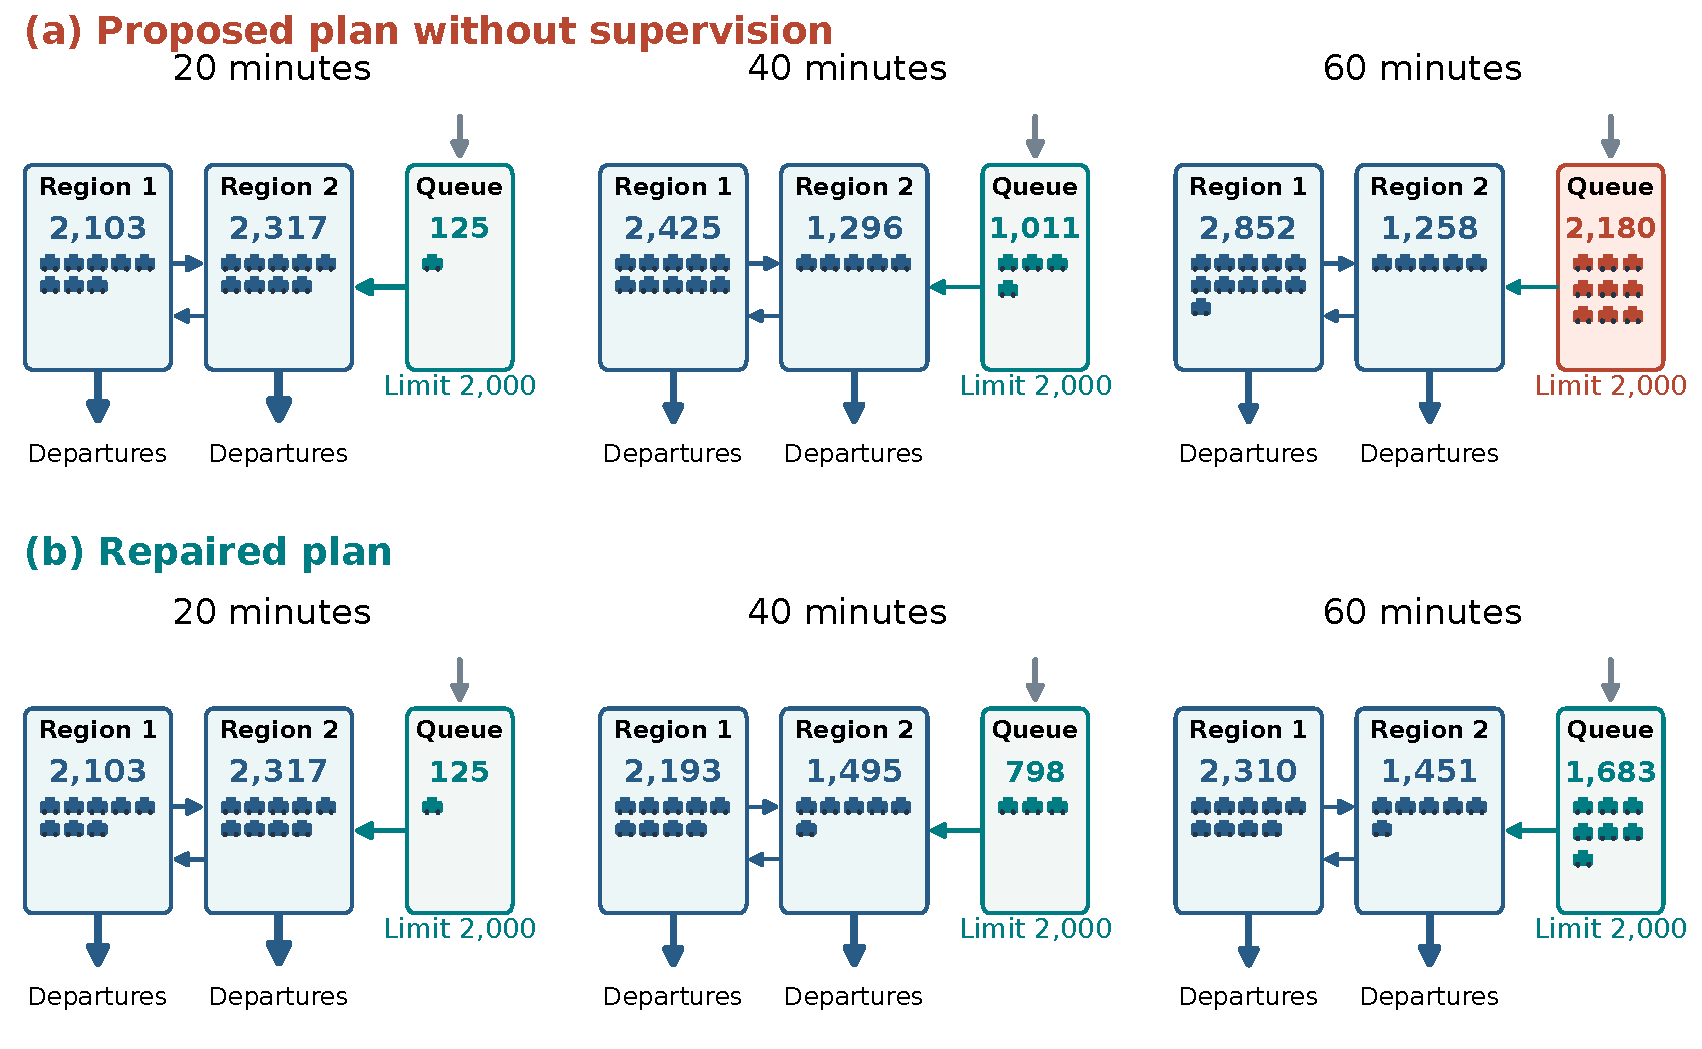
\includegraphics[width=\linewidth]{figures/supervisory_snapshots.pdf}
\caption{Traffic movements in the regional-priority study of
Section~\ref{sec:new-incident-protocol}. Both plans use the same
initial state at the upper bounds of the estimation box and constant
$+300$~veh/h arrival error. Numbers are
simulated vehicle counts rounded to whole vehicles. Each car icon
represents approximately 250 vehicles. Arrows show interregional
transfers, queue admission, exterior arrivals and departures, with
thickness proportional to the instantaneous rate on a common scale.
Departures combine local trip completion and exterior exits. Internal
demand is included in the simulation but omitted from the drawing.
Red identifies a queue above its 2000-vehicle capacity; icon positions
are illustrative.}
\label{fig:traffic-snapshots}
\end{figure}

\paragraph{Successive requests and computation delays}
\label{sec:sequential-handover-results}

Successive requests can change the regional priority while an earlier
plan is being executed. We compare implementing every proposed
replacement with activating only those accepted by the supervisory
agent. The trajectories and inputs are shown in
Figure~\ref{fig:successive-traffic}.
An initial
certified $p=4$ repair starts at minute~20. A $p=2$ full-scenario
proposal is accepted at minute~25, whereas a $p=4$ nominal proposal
is rejected at minute~30. The example uses
$(d,\bar w,\eta)=(1,300,2750)$, with replacements checked from
containing reachable-state boxes and the original minute-60 deadline.

Unchecked switching reduces admission and transfer from Region~1 at
minute~30, eventually exceeding queue capacity by about 5.6 vehicles.
This is a small overflow, at 0.28\% of storage. Retaining the accepted
plan avoids it, illustrating acceptance followed by rejection. Across 640 matched
simulations, supervised execution meets all requirements, compared with
512 for unchecked switching. Its median TTS is 8.2\% below retaining
the initial plan, with a 5.2\% greater priority cost than unchecked
switching. Costs use the requested weights over their respective
intervals. This is the first overflow example in a scan of 36 scenario
pairs, of which 30 permit the initialized sequence and three overflow
under unchecked switching. The other two overflowing pairs use initial
error bounds of 10 and 25 vehicles and reach overflows of 9.6 and
17.6 vehicles, respectively. In both, the supervisor rejects both
requests and continues the initial certified plan.

\paragraph{Computation delays}
\label{sec:delayed-handover-results}
Seventeen scenarios listed in \appref{app:sequential-handover} compare
one-, two- and five-minute activation delays. The current plan executes
while its future state set is propagated and a replacement is computed.
Eight replacements are ready and certified for the one-minute start,
and eleven for each longer delay. Three results miss the one-minute
start because computation is unfinished. In all other late or
inconclusive cases, the current plan continues. Every executed schedule
meets the requirements across 10,880 simulations per delay. More time
for computation can therefore permit a replacement, but the later
traffic state and shorter remaining time to the deadline must also be
covered. Table~\ref{tab:activation-delay-results} gives the counts.

\begin{figure}[pos=!htb]
\centering
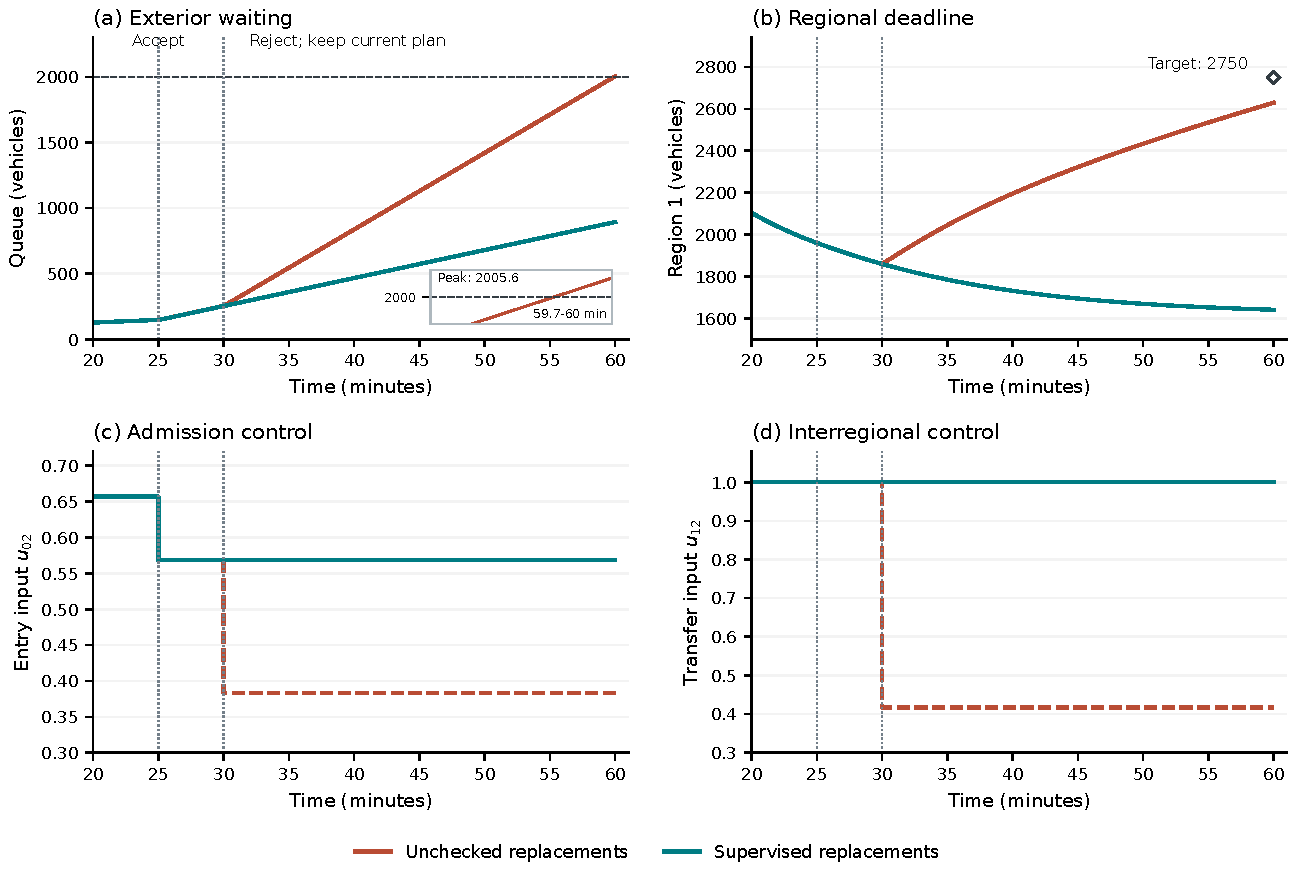
\includegraphics[width=0.94\linewidth]{figures/replanning_controls_2026_11_16.pdf}
\caption{Accepting and rejecting successive plan proposals under the
same traffic conditions. Both schedules start at minute~20 from
$x_0=\widehat x_{t_0}+d_x$, the upper bounds of the seven-component
state-estimation box, with $d_x=\mathbf1_7$ vehicles. Exterior arrivals
remain 300~veh/h above the forecast throughout. The supervisory agent
accepts the minute-25 plan and continues it after rejecting the
minute-30 proposal; unchecked implementation activates both. Panels (a)--(b) show queue length
and Region-1 accumulation, with queue capacity 2000 and a minute-60
target of 2750 vehicles. The inset resolves the unchecked queue peak
of approximately 2005.6 vehicles. Panels (c)--(d) show the entry input
$u_{02}$ and interregional input $u_{12}$; $u_{21}=u_{20}=1$
throughout. Vertical dotted lines mark the two request times.}
\label{fig:successive-traffic}
\end{figure}


\paragraph{Uncertainty, regional priority and deadline margins}
\label{sec:uncertainty-results}
The 80 regional-priority scenarios combine state-estimation bounds of
1--50 vehicles, arrival-error bounds of 60--300~veh/h, Region-1
deadline limits of 2750--2950 vehicles and weights $p=2,3,4$.
Here $d_x=d\mathbf1_7$, including the queue. Seventy-two settings
form the main grid, and eight additional validation settings use
intermediate values. The same planner and verification settings apply
to both sets. Figure~\ref{fig:acceptance-map} summarizes which proposals
can be implemented unchanged, with the full parameter map in
Figure~\ref{fig:acceptance-map-detail}. The requested priority is
decisive in this grid. All 36 full-scenario
proposals with $p=2$ are certified, including the largest tested
uncertainty bounds, and all eight with $p=3$ are certified. For $p=4$,
six of 36 pass, all with $d=1$ and $\bar w\le150$~veh/h.
\begin{figure}[pos=!htb]
\centering
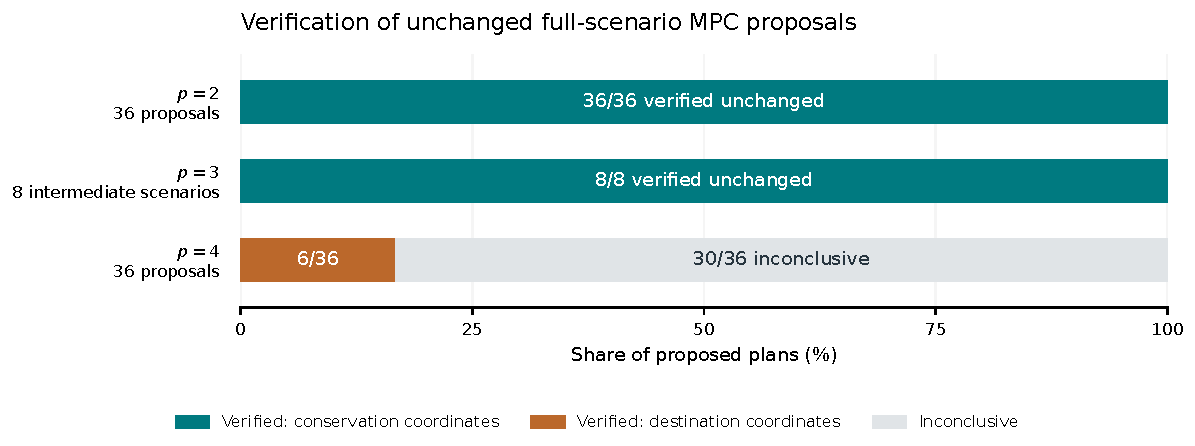
\includegraphics[width=0.96\linewidth]{figures/acceptance_by_priority_2026_11_16.pdf}
\caption{Verification of unchanged full-scenario MPC proposals, grouped
by the Region-2 priority weight $p$. Labels give the number of proposals
with each outcome divided by the number tested in that group. Teal
denotes verification with conservation coordinates, orange denotes
additional verification with destination coordinates, and gray denotes
inconclusive checks. The $p=2$ and $p=4$ groups each contain 36 settings
with initial error bounds of 1--50 vehicles and arrival-error bounds of
60--300~veh/h. The eight $p=3$ settings use intermediate parameter
values. All 80 proposals meet the requirements in their 640 sampled
simulations. Repair outcomes for nominal proposals are reported
separately in Table~\ref{tab:repair-outcomes};
Figure~\ref{fig:acceptance-map-detail} gives the full parameter map.}
\label{fig:acceptance-map}
\end{figure}

All 30 inconclusive proposals have $p=4$ and a smallest sampled
Region-1 deadline margin of approximately one vehicle, consistent with
the planner's clearance. Their continuous physical constraints pass,
but the regional deadline bound does not. The eight $p=3$ proposals
also approach the queue limit within one vehicle and still pass, so
margin size alone does not determine acceptance. The location of the
tight constraint and the accuracy of its bound both matter.

Figure~\ref{fig:acceptance-map-detail} gives the individual settings
behind the priority-group summary. Each point represents an unchanged
full-scenario MPC proposal checked with the same verification procedure.
\begin{figure}[pos=!htb]
\centering
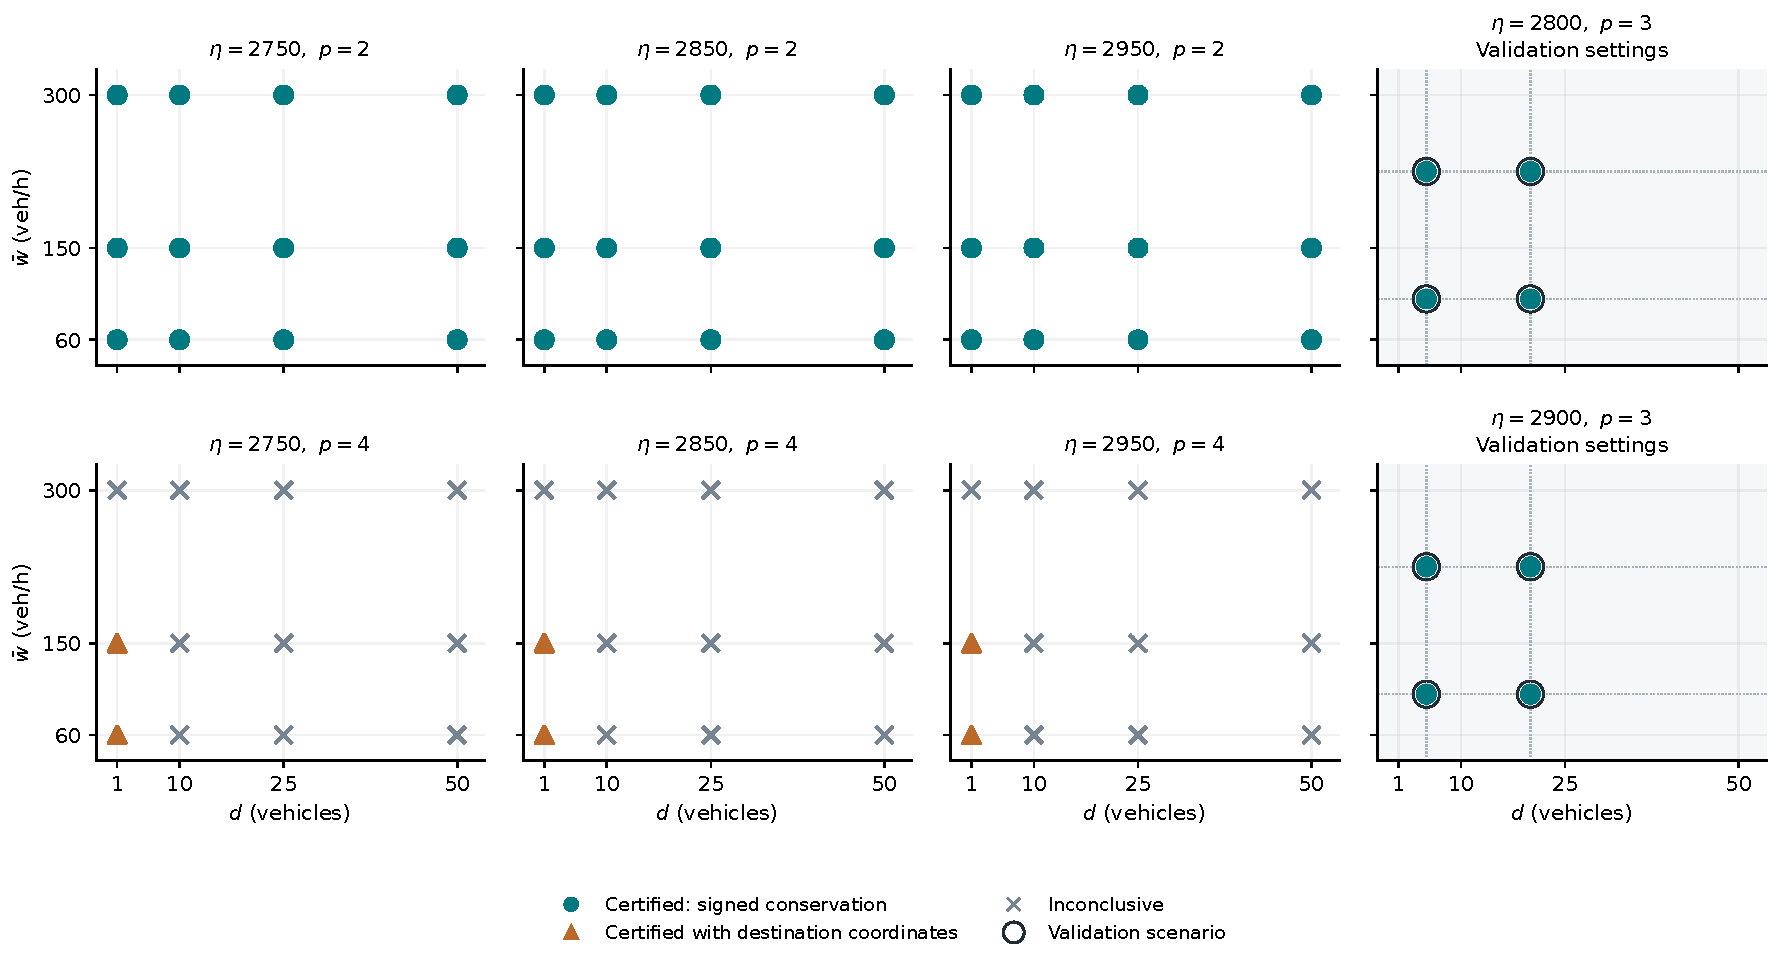
\includegraphics[width=\linewidth]{figures/acceptance_map.pdf}
\caption{Acceptance of full-scenario MPC proposals under different
regional priorities and service targets. Each panel fixes the
Region-1 limit $\eta$ at minute 60 and Region-2 priority weight $p$;
points vary the componentwise initial error bound $d$ and arrival-error
bound $\bar w$. Teal circles are certified with conservation coordinates,
orange triangles additionally require destination coordinates, and
gray crosses are inconclusive. Black outer circles identify additional
validation scenarios at intermediate parameter values, evaluated using
the same settings as the main grid. All 80 proposals satisfy every one of
their 640 sampled simulations. The result covers only the plotted
settings; stronger priority leaves little margin at the Region-1
deadline.}
\label{fig:acceptance-map-detail}
\end{figure}

\paragraph{Detailed outcomes of the numerical studies}
Tables~\ref{tab:benchmark-deadlines}--\ref{tab:benchmark-api-execution}
give the proposal, repair, delayed-implementation and agent outcomes
supporting Section~\ref{sec:new-evidence}. The corresponding protocols
and settings are in \appref{app:experimental-settings}.

\begin{table}[pos=!htb]
\centering\small
\caption{Proposals certified without change. Main grid and validation
columns count certificates in the 72 main grid and eight validation
cases; Total combines them. Simulation passes require all 640
simulations in a case to meet physical constraints and service
requirements. MPC denotes model predictive control. Signed denotes
signed conservation; Sequential denotes the sequential verification
procedure, which was evaluated for nominal and full-scenario proposals.}
\label{tab:benchmark-deadlines}
\label{tab:fixed-portfolio}
\begin{tabularx}{\linewidth}{@{}Xlrrrr@{}}
\toprule
Planner & Check & Main grid & Validation & Total & \shortstack{Simulation\\passes}\\
\midrule
Nominal MPC & Signed & 36/72 & 0/8 & 36/80 & 36/80\\
 & Sequential & 36/72 & 0/8 & 36/80 & 36/80\\
Five-scenario MPC & Signed & 36/72 & 4/8 & 40/80 & 40/80\\
Full-scenario MPC & Signed & 36/72 & 8/8 & 44/80 & 80/80\\
 & Sequential & 42/72 & 8/8 & 50/80 & 80/80\\
\bottomrule
\end{tabularx}
\end{table}

\begin{table}[pos=!htb]
\centering\small
\caption{Certified outputs after repair across the 80 test cases. Cases
with a certified output are counted out of all 80 cases. Simulation
passes count only the selected outputs and require all 640 simulations
in a case to meet physical constraints and service requirements.}
\label{tab:repair-outcomes}
\begin{tabularx}{\linewidth}{@{}Xrr@{}}
\toprule
Execution option & \shortstack{Cases with a\\certified output} &
\shortstack{Simulation\\passes}\\
\midrule
Nominal MPC with repair & 74/80 & 74/74\\
Full-scenario MPC with repair & 74/80 & 74/74\\
Repair with new backup & 80/80 & 80/80\\
\bottomrule
\end{tabularx}
\end{table}

\begin{table}[pos=!htb]
\centering\small
\caption{Delayed activation across seventeen test cases per delay. Timely
replacements have a matching certificate ready by the plan start time; inconclusive
or late results retain the current plan. Each executed schedule is tested
on 640 simulations, giving 10,880 simulations per delay.}
\label{tab:activation-delay-results}
\begin{tabular}{@{}rrrr@{}}
\toprule
\shortstack{Delay\\(minutes)} & \shortstack{Timely\\replacements} &
\shortstack{Current plan\\continued} & \shortstack{Simulation\\passes}\\
\midrule
1 & 8/17 & 9/17 & 10,880/10,880\\
2 & 11/17 & 6/17 & 10,880/10,880\\
5 & 11/17 & 6/17 & 10,880/10,880\\
\bottomrule
\end{tabular}
\end{table}

\begin{table}[pos=!htb]
\centering\small
\caption{Agent planning under corrupted memory, with four histories per
format. History only supplies instructions and interaction history; Task
record additionally supplies the current priority and timing. Objective
correct counts traces matching the operator's priority. Repairs executed
counts traces activating a checked repair. Feasible trajectories satisfy
physical and service requirements across $4\times640=2560$ simulations
per format.}
\label{tab:benchmark-api-execution}
\begin{tabularx}{\linewidth}{@{}Xrrr@{}}
\toprule
Format & \shortstack{Objective\\correct} & \shortstack{Repairs\\executed} & \shortstack{Feasible\\trajectories}\\
\midrule
History only & 1/4 & 1/4 & 2560/2560\\
Task record & 4/4 & 4/4 & 2560/2560\\
\bottomrule
\end{tabularx}
\end{table}

\paragraph{Queue violation in the congested case}
\label{app:congested-diagnostics}
Since $a\le\kappa_{02}u_{02}$, the queue at one hour satisfies
\[
z(1)\ge z(0)+\int_0^1\Lambda(t)\,dt
             -\kappa_{02}\int_0^1u_{02}(t)\,dt.
\]
With initial queue 510 vehicles and constant arrival error
$+600$~veh/h, exact arithmetic on the implemented coefficients gives
a lower bound above 2022 vehicles at repair weight 0.60. This bound also
exceeds 2000 vehicles at every smaller grid weight. Weight 0.65
has a full-hour certificate. Thus the rejection of earlier candidates
is established by a violation, not only by an inconclusive check.

\paragraph{Sensitivity to model error}
\label{sec:plant-sensitivity-results}
\label{app:plant-sensitivity}
A companion congested case tests sensitivity to errors in the traffic
model, using the initial condition, state-error bounds and backup of
Section~\ref{sec:congested-results}, a 300~veh/h arrival-error bound,
and a certified repaired plan with $\lambda_{\rm rep}=0.35$. We keep
both plans fixed while perturbing MFD outflow and internal
demand independently by $-5\%$, zero and $+5\%$, giving nine simulated
plants. Backup meets physical and service requirements in all 5760
simulations. The repaired plan respects physical limits throughout but
misses the Region-1 deadline in 280 simulations, all with 5\% lower
outflow and 5\% higher internal demand together.

Additional internal trips and reduced discharge both slow regional
recovery, and the fixed inputs do not adapt to these changes. The
largest deadline accumulation is approximately 2356 vehicles with
lower outflow alone and 2137 with higher internal demand alone, compared
with 4174 when combined, against a target of 3300 vehicles. The combined
effect is therefore substantially larger than either individual effect.
These perturbations lie outside the certified model: coverage of state
and arrival errors does not cover errors in regional outflow and
internal demand. Those effects require additional model-error bounds.
Each plan is evaluated on 128 initial-state corners and five arrival
profiles for each of the nine plants. Halving the integration step
from 2.5 to 1.25 seconds for the adverse combination preserves the
pass counts and changes the largest Region-1 deadline accumulation
by less than 0.1 vehicles. This is a sensitivity test of the aggregate
model, rather than microsimulation validation.

\paragraph{Network efficiency under different arrival increases}
\label{sec:network-efficiency-comparison}
A separate comparison minimizes network-wide TTS without a regional
service deadline. Twelve scenarios combine arrival increases of
20--50\% with durations of 30, 45 and 60 minutes, one-vehicle state
errors and a 300~veh/h arrival-error bound. This comparison pairs
sixteen initial-state corners with the five arrival profiles per scenario.
All MPC proposals pass unchanged. Table~\ref{tab:arrival-efficiency}
shows median paired TTS reductions of 23.5--24.5\% across the four arrival
increases, relative to the locally implemented extension of Zhong
et al.'s CLF controller~\cite{zhong2018robust}. Across all 960 matched
simulations, the median reduction is 24\%. This gain is produced by
planning and preserved by verification. The controller includes
queue and exterior-exit feedback added for this model, so the result
is specific to that implementation and comparison; its settings are
given in \appref{app:experimental-settings}.

\begin{table}[pos=!htb]
\centering\small
\caption{Network-efficiency comparison grouped by exterior-arrival
increase. Each row pools three durations (30, 45 and 60 minutes),
sixteen initial-state corners and five arrival-error profiles, giving
240 matched simulations. TTS is evaluated over minutes 20--60 and
reported as a median in veh-h. The last column is the median percentage
reduction computed separately for each matched pair. CLF denotes the
locally extended controller described in Appendix~\ref{app:experimental-settings}.
All MPC plans are certified without modification.}
\label{tab:arrival-efficiency}
\begin{tabularx}{\linewidth}{@{}Xrrr@{}}
\toprule
Arrival increase & MPC TTS & CLF TTS & Paired reduction (\%)\\
\midrule
20\% & 2568 & 3357 & 23.5\\
30\% & 2645 & 3474 & 23.9\\
40\% & 2724 & 3593 & 24.3\\
50\% & 2807 & 3716 & 24.5\\
\bottomrule
\end{tabularx}
\end{table}

\paragraph{Several entry queues}
\label{app:network-transfer}
The ring model has $N=2$ or $3$ regions, destination-specific
accumulations $n_{ij}$, and one queue $z_i$ per region. Regions and
destinations are indexed by $1,\ldots,N$, with regional total
$n_i=\sum_{j=1}^N n_{ij}$. Local completion is $n_{ii}v(n_i)$.
Nonlocal vehicles move to the next region in the directed ring,
from $i$ to $i+1$ and from $N$ to $1$, while retaining their destination.
Writing $u_i^{\rm ring}$ for this input, their transfer rate is
$u_i^{\rm ring}n_{ij}v(n_i)$ for $j\ne i$. Admission is
$a_i=\min\{60z_i,12{,}000u_i^{\rm in}\}$. Half the admitted traffic
is local and the rest is equally divided among other destinations.
Internal demand in each region is 6000 local veh/h plus a total of
500 nonlocal veh/h, divided equally among other destinations.
Regional and queue capacities are 10,000 and 2000 vehicles.

The recovery in Figure~\ref{fig:three-region-traffic} uses $N=3$,
4500 initial vehicles per region, half local and the rest equally
divided between the other destinations, and 500 per queue. The
forecast is 6000~veh/h per queue, increased to 7800 at Queue~1 over
minutes 15--45. Ring inputs remain one. All entrance inputs are zero
over minutes 0--5. Over minutes 5--60, the proposal uses
$(u_1^{\rm in},u_2^{\rm in},u_3^{\rm in})=(0.495,0.50,0.50)$ and the
backup uses $(0.55,0.50,0.50)$. These plans are prescribed. Region-1
priority is measured by
$\int_0^1(4n_1+n_2+n_3+z_1+z_2+z_3)\,dt$.
The selected repair has weight 0.45 and entry inputs
$(0.51975,0.50,0.50)$. Verification uses independent initial errors
of $25/3$ vehicles per destination accumulation and 10 per queue,
independent arrival errors bounded by 300~veh/h per queue, and a
3300-vehicle deadline in every region at one hour.

For the allowed initial Queue~1 value of 510 vehicles and constant
$+300$~veh/h arrival error, the queue receives 7200 vehicles over the
hour. Admission is at most $12{,}000(0.495+0.055\lambda_{\rm rep})$ veh/h
after minute~5, where $\lambda_{\rm rep}$ is the repair weight. Hence
\[
z_1(1)\ge7710-11{,}000(0.495+0.055\lambda_{\rm rep}).
\]
This exceeds 2000 for every tested weight at or below 0.40; at 0.40
the bound is approximately 2023. Exact checks use the implemented
binary input coefficients. Weight 0.45 passes all physical and
service checks. Admission remains capacity-limited throughout the
verified uncertainty family, so the entrance inputs determine the
regional admission rates while arrival error affects the queues.

Traffic performance is compared on 64 matched simulations per plan:
four combinations of upper/lower initial states and constant
positive/negative arrival errors, the nominal case, and 59 random
initial states with independent five-minute arrival-error blocks
(seed 20261116). DOP853 integration uses a maximum step of 15~s
and splits at every change in inputs, arrival forecasts or error
profiles. All simulated repaired-plan counts lie within the
verified bounds. For the illustrated adverse simulation, repair retains
59.3\% of the proposal's priority-cost reduction relative to backup,
with 0.22\% lower TTS than backup. Verification of each of the repaired
and backup plans took about 12.4~s in these runs. Regional-total
initial-error bounds of 50 and 75 vehicles were also tested for this
backup and remained inconclusive. The deadline bounds have substantial
slack; the result does not establish the largest admissible uncertainty.

The supporting two- and three-region ring comparisons start with
3000 vehicles per region, half local, and 200 per queue. Arrivals
are 4000~veh/h per queue with the same 30\% increase at Queue~1 over
minutes 15--45. Ring/entrance inputs start at 0.65/0.50. After
minute~30, ring inputs 1/2 become 0.80/0.55 and entrance input~1
becomes 0.60, with other inputs unchanged. Initial errors are $25/N$
vehicles per destination and 10 per queue. Per-queue arrival-error
bounds are 300 and 60~veh/h for the two- and three-region cases,
respectively. Conservation coordinates certify both fixed plans
against 2700-vehicle regional deadlines at one hour. The largest
deadline bounds are 1552 and 2060 vehicles, respectively, rounded
upward; destination-coordinate checks are inconclusive in these
supporting cases.


\paragraph{AI interpretation of operator instructions}
\label{sec:task-state-live}
Four operator histories under corrupted memory compare an agent given
interaction history alone with one also given an explicit task record.
Correct objective selection increases from one of four histories to
all four with the record. In one history, Region-2 priority should
resume after a temporary Region-1 priority ends. History alone selects
the wrong objective, while the task record leads to the intended
priority and a successful repair. The supervisor maintains physical
and service requirements across all 2560 simulations per format,
including those with the wrong objective. The demonstration separates
instruction interpretation from constraint satisfaction, as in
Corollary~\ref{cor:agent-independent-execution}. The eight traces use
one agent model, with protocol and outcomes in
\appref{app:agent-evaluation} and Table~\ref{tab:benchmark-api-execution}.

A complementary 96-query pilot selects among precomputed plans.
Task records give 24/24 correct objectives under both clean and
corrupted memory, compared with 19/24 and 15/24 for history alone,
respectively (\appref{app:interpretation-pilot}). These queries repeat
a small set of histories and test interpretation and tool selection,
rather than the fresh planning and repair used in the live study.

\paragraph{Stored-plan interpretation pilot}
\label{app:interpretation-pilot}
This separate pilot uses the same agent model to select among
precomputed plans. It crosses three tool-availability situations, four
operator histories, clean or corrupted memory, two input formats, and
two repetitions, giving 96 model queries. The stored situations are a
network-efficiency MPC plan with a 20\% arrival increase lasting
30 minutes, a repair case with
$(d,\bar w,\eta,p)=(1,60,2750,4)$, and that repair case with replacement
tools unavailable. Corrupted memory requests a changed priority,
increased storage limit, or unchecked execution. Objective correctness
is measured against the active instruction. Tool correctness follows
the stored selection order: certified network-efficiency MPC,
certified scenario MPC, checked repair, then continuation of the
current plan.

Task records give 24/24 correct objectives under both clean and
corrupted memory, compared with 19/24 and 15/24 for history alone.
These pilot outcomes and the live planning traces are demonstrations
on one model and a limited set of histories.

\bibliographystyle{elsarticle-num}
\setlength{\bibsep}{0pt}
\bibliography{FOUNDATION_REFERENCES}
\end{document}
